\begin{savequote}[75mm]
Mathematics knows no races or geographic boundaries; for mathematics, the cultural world is one country.
\qauthor{--- David Hilbert ---}
\end{savequote}

\chapter{Functions}
\label{chap_functions}
\graphicspath{{figures/Functions/}}
\section{The Cartesian coordinate plane}
\label{CartesianPlane}

\ifcourse
In order to visualize the pure excitement that is calculus, we need to unite algebra and geometry.  Simply put, we must find a way to draw algebraic things.  Let us start with possibly the greatest mathematical achievement of all time: the \index{Cartesian coordinate plane} \textbf{Cartesian coordinate plane} (\textit{Cartesisch co\"ordinatenstelsel})\index[aut]{Cartesisch co\"ordinatenstelsel}. So named in honour of Ren\'{e} Descartes. 
\fi
\ifvc
We must find a way to draw algebraic things.  Let us start with possibly the greatest mathematical achievement of all time: the \index{Cartesian coordinate plane} \textbf{Cartesian coordinate plane}  (\textit{Cartesisch co\"ordinatenstelsel}) \index[aut]{Cartesisch co\"ordinatenstelsel}. So named in honour of Ren\'{e} Descartes. 
\fi


Imagine two real number lines crossing at a right angle at $0$. The horizontal number line is usually called the \index{$x$-axis}\index[aut]{$x$-as}\textbf{\boldmath $x$-axis} (\textit{$x$-as}), while the vertical number line is usually called the \index{$y$-axis}\index[aut]{$y$-as}\textbf{\boldmath $y$-axis} (\textit{$y$-as}). For example, consider the point $P$ in Figure~\ref{fig_functions_1}.  To use the numbers on the axes to label this point, we project the point $P$ to the $x$- (respectively $y$-) axis.  We then describe the point $P$ using the \index{ordered pair} \textbf{ordered pair} (\textit{geordend koppel}) $(2,-4)$.\index[aut]{geordend koppel}  The first number in the ordered pair is called the\index{abscissa}\index[aut]{abscis} \textbf{abscissa} (\textit{abscis}) or \index{$x$-coordinate} \textbf{\boldmath $x$-coordinate} and the second is called the \index{ordinate} \textbf{ordinate} (\textit{ordinaat}) or \index{$y$-coordinate}\index[aut]{ordinaat}\textbf{\boldmath $y$-coordinate}. When we speak of the Cartesian coordinate plane, we mean the set of all possible ordered pairs $(x,y)$ as $x$ and $y$ take values from the real numbers.  The ordered pair $(2,-4)$ comprise the \index{Cartesian coordinates}\index[aut]{Cartesische co\"ordinaten}\textbf{Cartesian coordinates} (\textit{Cartesische co\"ordinaten}) of the point $P$. In practice, the distinction between a point and its coordinates is blurred.  We can think of $(2,-4)$ as instructions on how to reach $P$ from the \index{origin}\index[aut]{oorsprong}{\bf origin} (\textit{oorsprong}) $(0, 0)$. 


\begin{figure}
	\begin{center}
			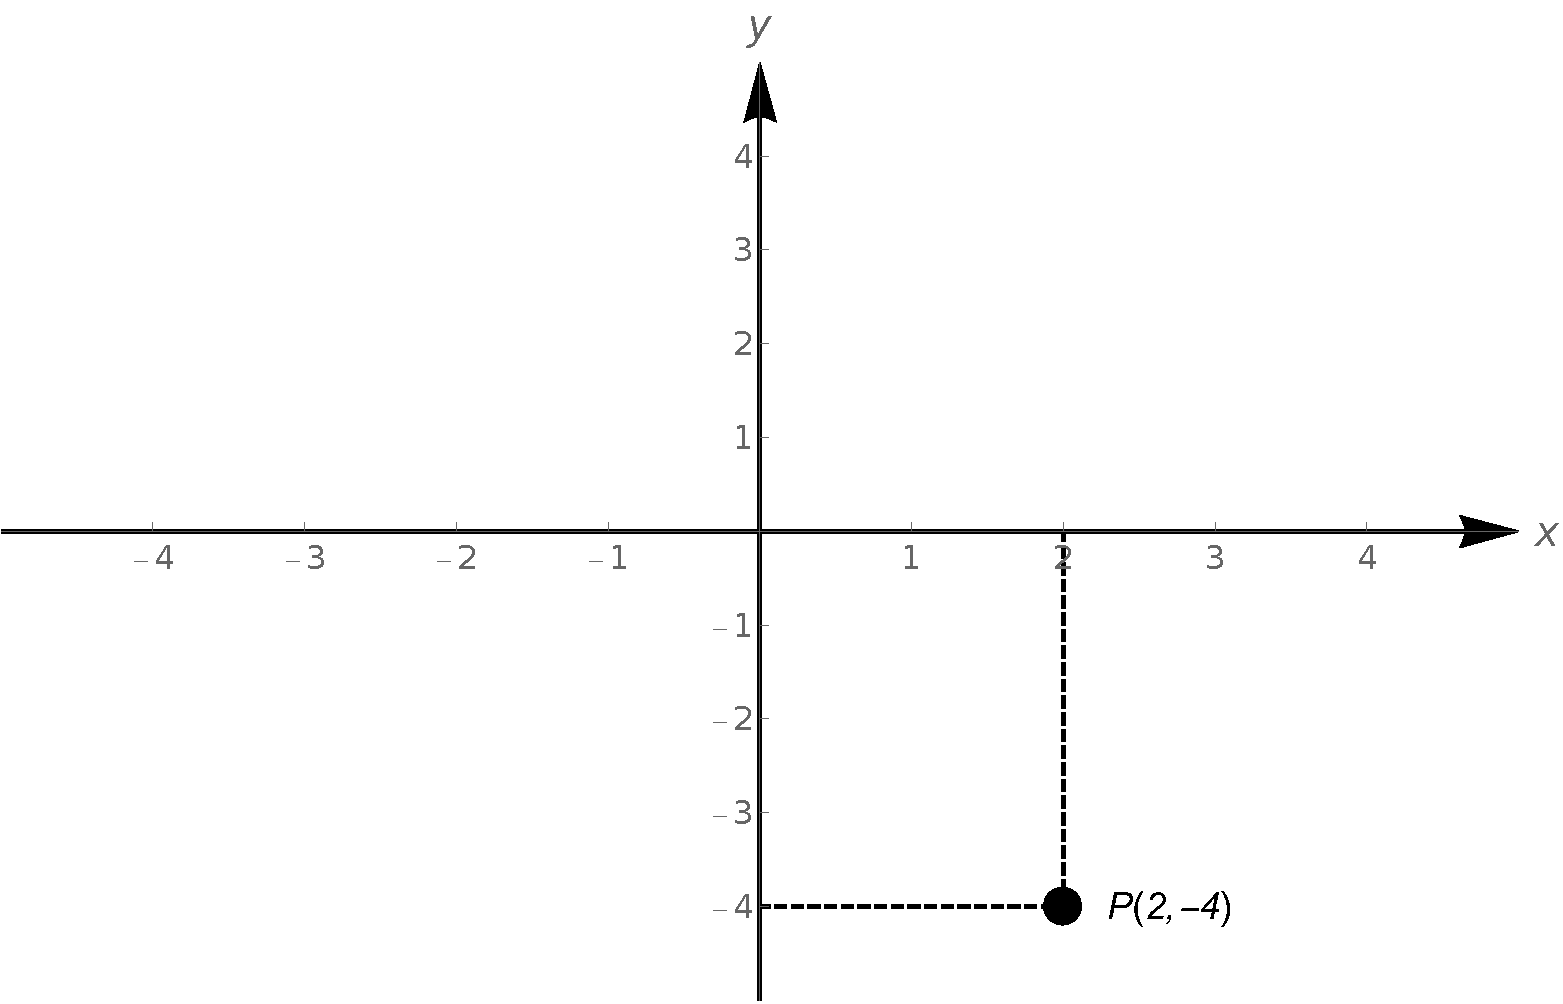
\includegraphics[width=0.5\textwidth]{fig_functions_1}
	\caption{The point $P$ located in the Cartesian coordinate plane.}
	\label{fig_functions_1}
	\end{center}
\end{figure}


\ifvc
 Moreover, we observe that
\begin{itemize}

\item $(a,b)$ and $(c,d)$ represent the same point in the plane if and only if $a = c$ and $b = d$.

\item  $(x,y)$ lies on the $x$-axis if and only if $y = 0$.

\item  $(x,y)$ lies on the $y$-axis if and only if $x=0$.

\end{itemize}
\fi



The axes divide the plane into four regions called \index{quadrants} \textbf{quadrants} (\textit{kwadrant})\index[aut]{kwadrant}.  They are labelled with Roman numerals and proceed counter-clockwise around the plane \ifvc (Figure~\ref{fig_functions_2})\fi. If a point other than the origin happens to lie on the axes, we typically refer to that point as lying on the positive or negative $x$-axis (if $y = 0$) or on the positive or negative $y$-axis (if $x = 0$).   Such points do not belong to any of the four quadrants.




Using Cartesian coordinates, we can introduce the three main types of \textbf{symmetry} (\textit{symmetrie}), namely symmetry about the $x$-axis, symmetry about the $y$-axis, and finally, symmetry about the origin. \index{symmetry}\index[aut]{symmetrie}


\ifvc
\begin{definition}[Symmetry of points]
Two points $(x_1,y_1)$ and $(x_2,y_2)$ in the plane are said to be
\vspace{-0.3cm}
\begin{itemize}
\item symmetric about the  $x$-axis if $x_1 = x_2$ and $y_1 = -y_2$;
\item symmetric about the $y$-axis if $x_1 = -x_2$ and $y_1 = y_2$;
\item symmetric about the origin if $x_1 = -x_2$ and $y_1 = -y_2$.
\end{itemize}
\end{definition}
The concept of symmetry is illustrated in Figure~\ref{fig_functions_3}. In that figure, $P$ and $S$ are symmetric about the $x$-axis, as are $Q$ and $R$;  $P$ and $Q$ are symmetric about the $y$-axis, as are $R$ and $S$;  and $P$ and $R$ are symmetric about the origin, as are $Q$ and $S$.

\begin{figure}[H]
	\begin{center}
			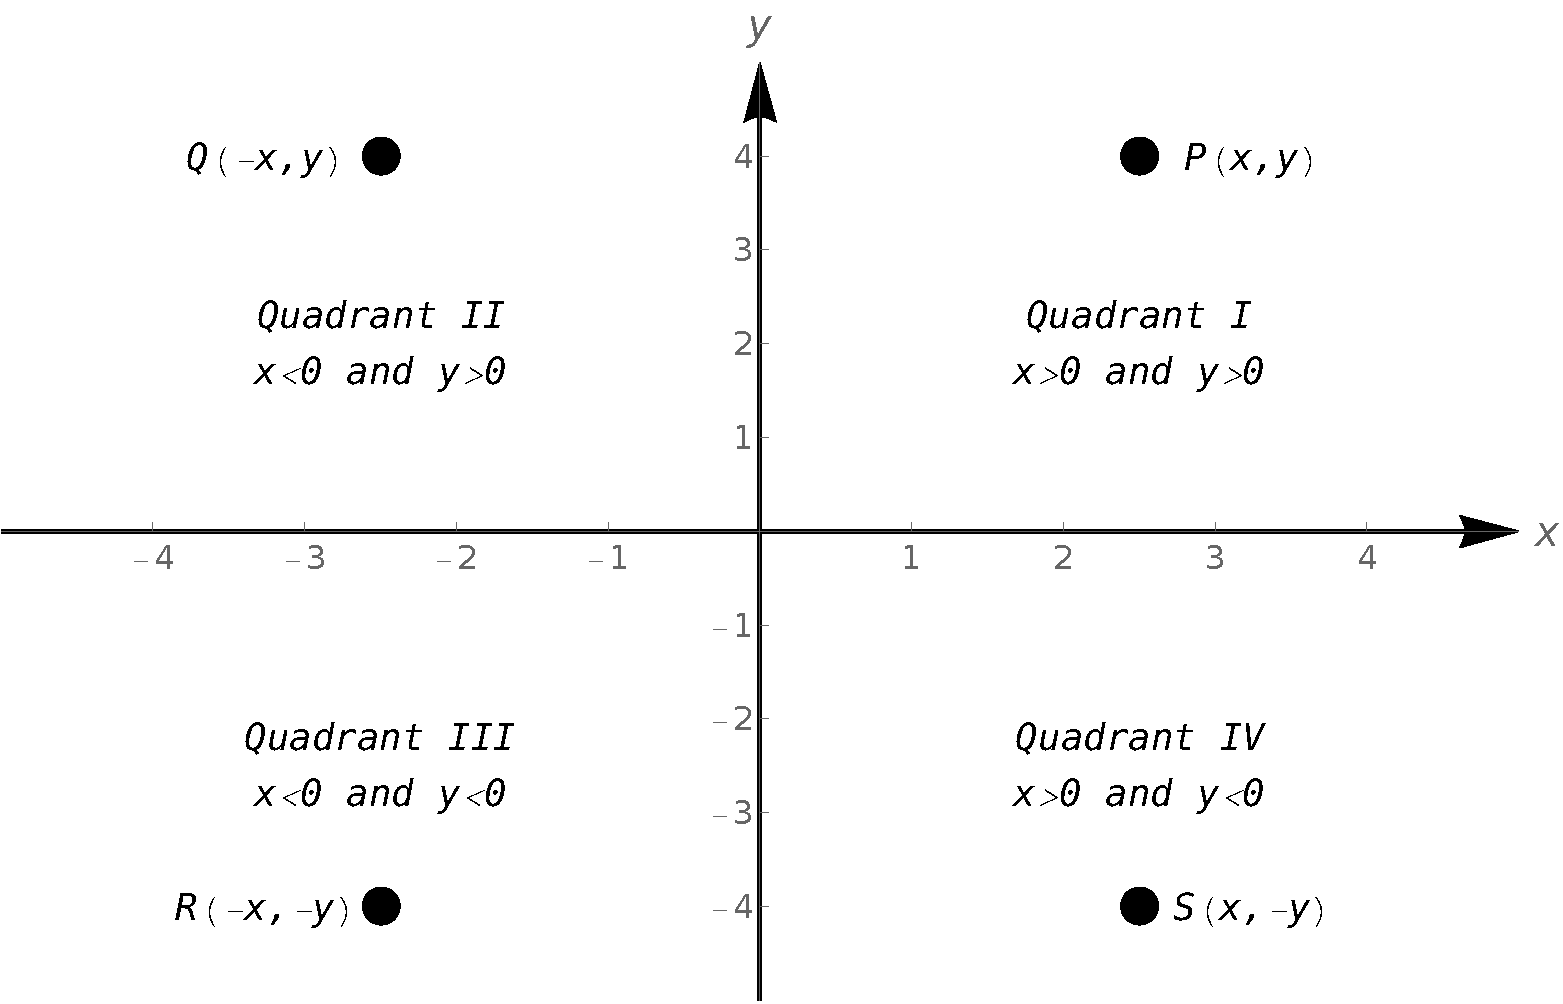
\includegraphics[width=0.5\textwidth]{fig_functions_2}
	\caption{The quadrants and symmetry of points in the Cartesian coordinate plane.}
	\label{fig_functions_2}
	\end{center}
\end{figure}

\ifvc\pagebreak\fi
\begin{example}
Let $P$ be the point $(-2,3)$.  Find the points that are symmetric to $P$ about the:

\begin{multicols}{3}

\begin{enumerate}

\item  $x$-axis,

\item  $y$-axis,

\item  origin.

\end{enumerate}

\end{multicols}

\xhrulefill{gray}{2.5pt}Solution \xhrulefill{gray}{2.5pt}


\begin{enumerate}

\item  To find the point symmetric about the $x$-axis, we replace the $y$-coordinate with its opposite to get  $(-2,-3)$. 

\item  To find the point symmetric about the $y$-axis, we replace the $x$-coordinate with its opposite to get $(2,3)$. 

\item  To find the point symmetric about the origin, we replace the $x$- and $y$-coordinates with their opposites to get $(2,-3)$. Here, we reflect across the $x$-axis and then across the $y$-axis. 

\end{enumerate}
\end{example}


\fi


\section{Functions}
\subsection{Relations}
\label{relaties}
\begin{definition}[Relation]
A \index{relation}\index[aut]{relatie} \textbf{relation} (\textit{relatie}) is a set of points in the plane. Hence,  a relation $R$ in $\mathbb{R}$ is a subset of the Cartesian product $\mathbb{R}^2$. 
\end{definition}


Since relations are sets, we can describe them using the techniques presented in Chapter~\ref{SetsChapter}.  That is, we can describe a relation verbally, using the roster method, or using set-builder notation. Most frequently, the latter kind of description is preferred and a relation is defined using a specific predicate that depends on $x$ and $y$, $P(x,y)$, i.e. \index{verbal method}\index{roster method}\index{set-builder notation}
$$
R=\left\{(x,y)\in\mathbb{R}^2\mid P(x,y) \right\}\,.
$$

The predicate  $P(x,y)$ is the rule that allows us to select the ordered pairs $(x,y)$ that make up the relation. Here, we call $x$ the \textbf{argument} (\textit{argument}) of the relation $R$ and $y$ its corresponding \textbf{image} (\textit{beeld}). Since the elements in a relation are points in the plane, we often try to describe the relation graphically as well.  Doing so produces the \textbf{graph} (\textit{grafiek}) of the relation $R$.
\index{image}\index[aut]{beeld}
\index{argument}\index[aut]{argument}
\index{graph}\index[aut]{grafiek}


\begin{example}
 Graph the following relations. \label{relationgraphingexample}



\begin{multicols}{2}
\begin{enumerate}
\ifvc
\item  $A = \{ (0,0), (-3,1), (4,2), (-3,2)\}$
\fi
\item  $B = \{ (x,3) \, | \, -2 \leq x \leq 4\}$
\item  $C = \{ (3,y) \, | \, \mbox{$y$ is a real number} \}$
\end{enumerate}
\end{multicols}

\ifvc\pagebreak\fi
\xhrulefill{gray}{2.5pt}Solution \xhrulefill{gray}{2.5pt}

\begin{enumerate}
\ifvc
\item  To graph $A$, we simply plot all of the points which belong to $A$, as shown in Figure~\ref{fig_functions_3a}.
\fi
\item  In words,  $\{ (x,3)\, | \, -2 \leq x \leq 4 \}$  reads `the set of points $(x,3)$ such that $-2 \leq x \leq 4$. Plotting several representative points should convince you that $B$ describes the horizontal line segment from the point $(-2,3)$ up to and including the point $(4,3)$ (Figure~\ref{fig_functions_3b}).
\item  The relation $C$ is  described as the set of points $(3,y)$ such that $y$ is a real number.  All of these points have an $x$-coordinate of $3$, but the $y$-coordinate is free to be whatever it wants to be, without restriction. Hence, all the points of $C$ lie on the vertical line  $x = 3$ (Figure~\ref{fig_functions_3c}).  

\end{enumerate}

\ifvc
\begin{figure}[H]
\centering
%\raisebox{0.5cm}{
\centerline{
\subfigure[Set $A = \{ (0,0), (-3,1), (4,2), (-3,2)\}$ \label{fig_functions_3a}]{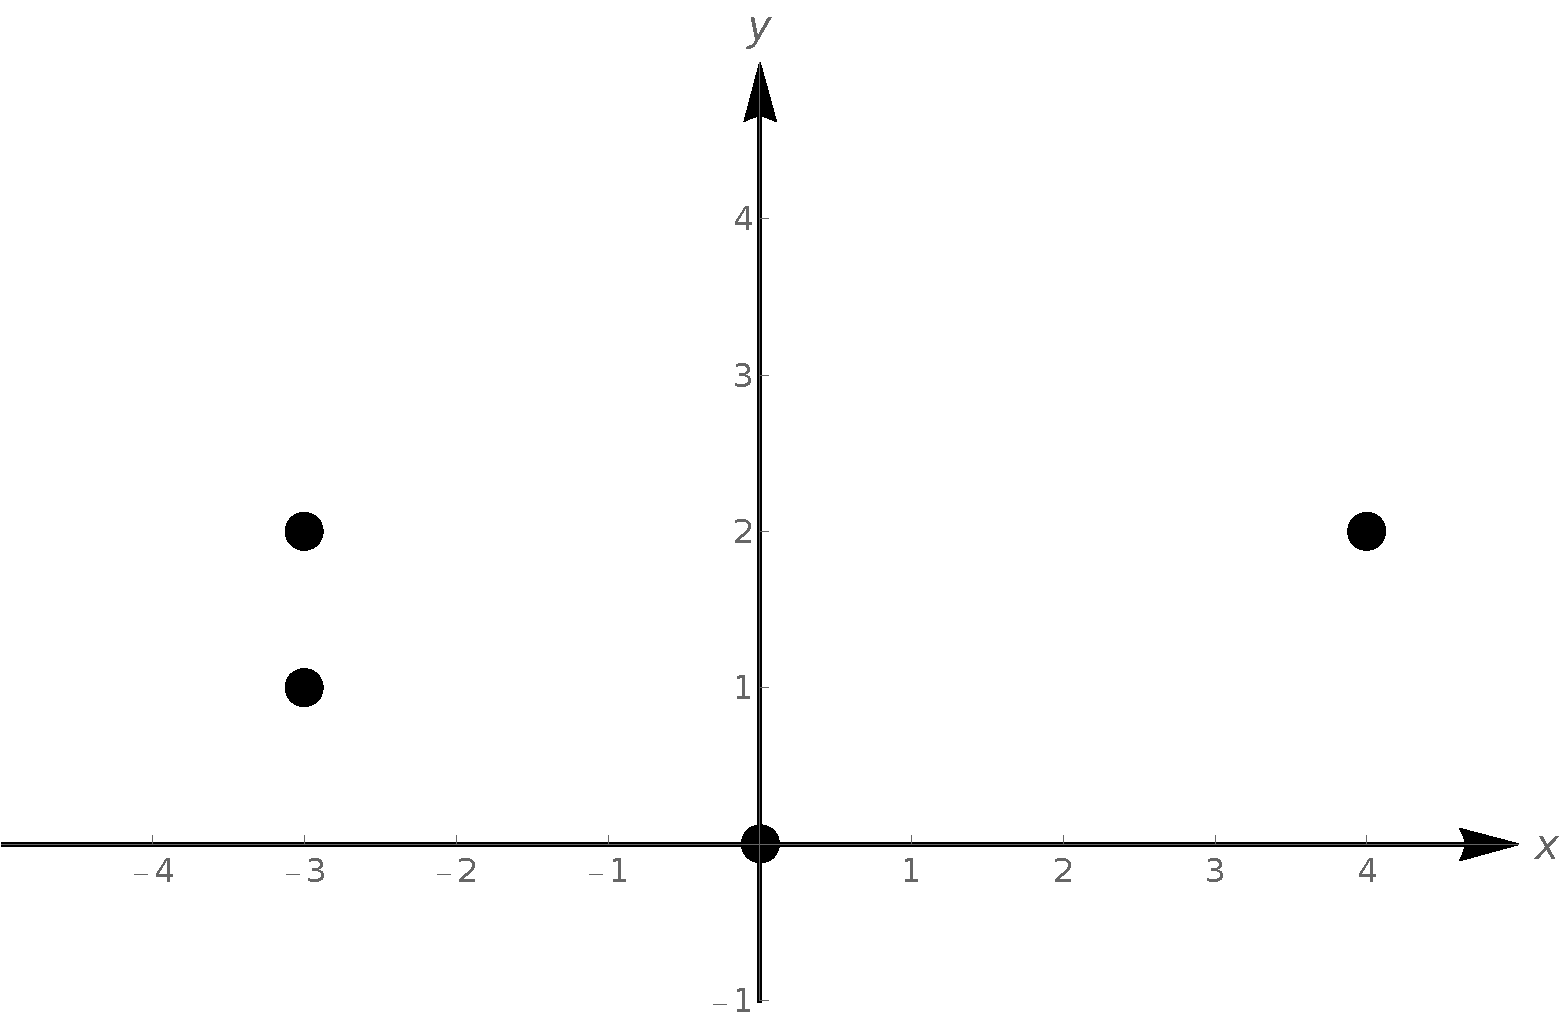
\includegraphics[width=0.4\textwidth]{fig_functions_3a}}
\hspace{0.1cm}
\subfigure[Set $B = \{ (x,3) \, | \, -2 \leq x \leq 4\}$ \label{fig_functions_3b}]{\includegraphics[width=0.4\textwidth]{fig_functions_3b}}
}
\centerline{
\subfigure[Set $C = \{ (3,y) \, | \, \mbox{$y$ is a real number} \}$ \label{fig_functions_3c}]{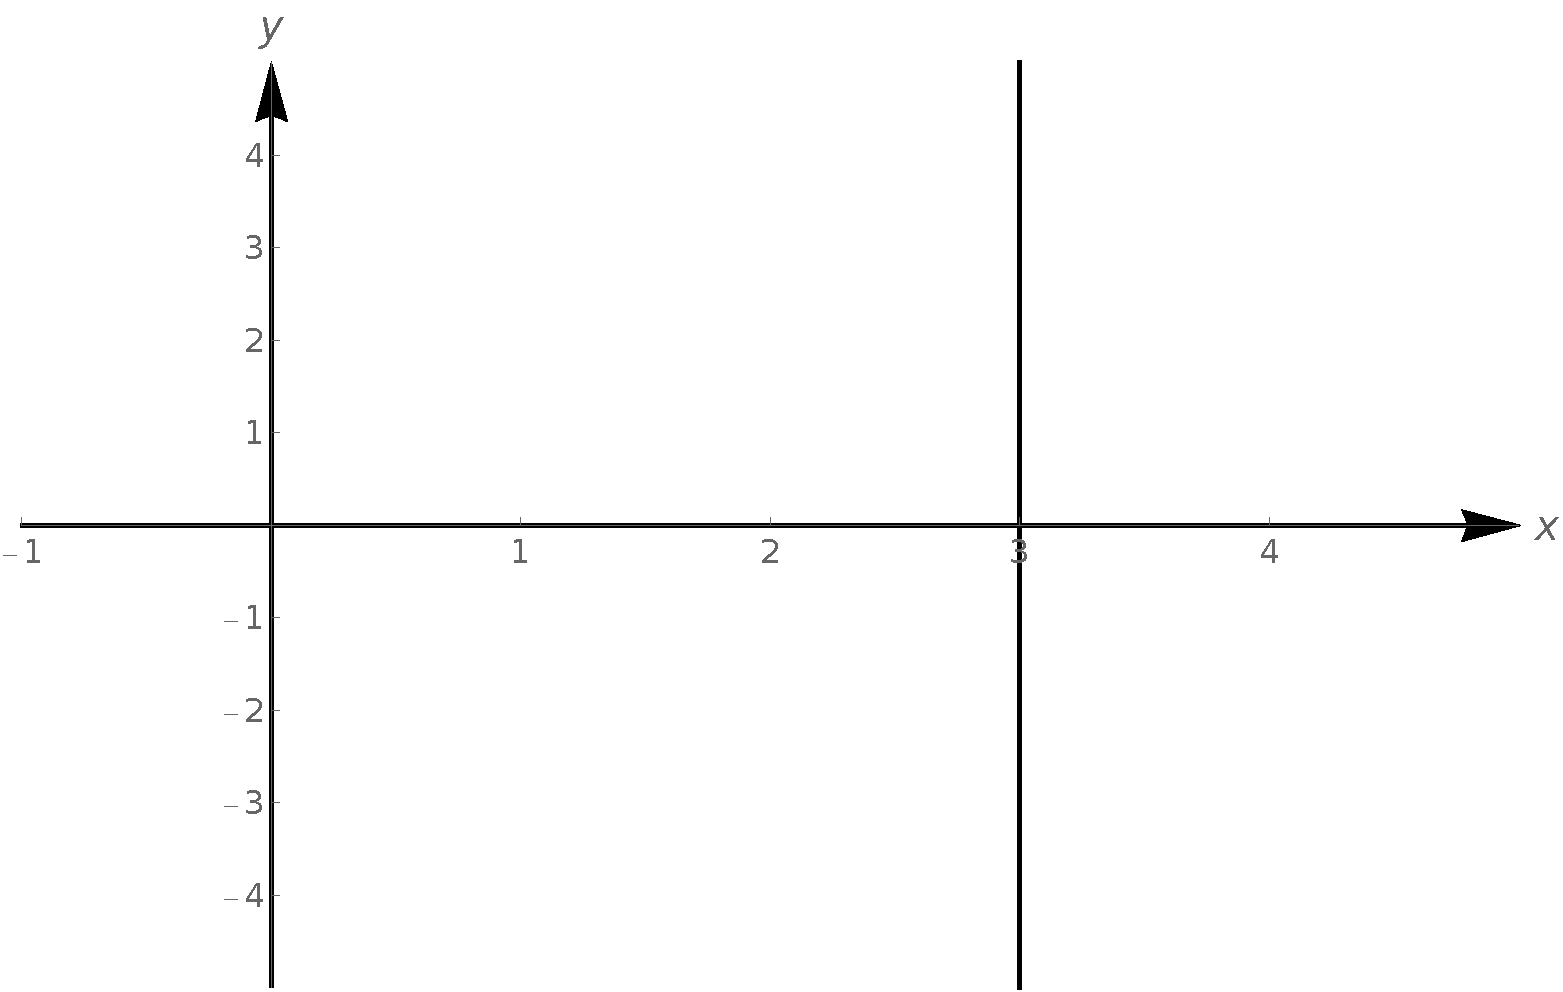
\includegraphics[width=0.4\textwidth]{fig_functions_3c}}
}
\caption{Graphs of different relations.} 
\end{figure}
\fi



\ifcourse
\begin{figure}[H]
\centering
%\raisebox{0.5cm}{
\centerline{
\subfigure[Set $B = \{ (x,3) \, | \, -2 \leq x \leq 4\}$ \label{fig_functions_3b}]{\includegraphics[width=0.4\textwidth]{figures/Functions/fig_functions_3b.pdf}}
\hspace{0.1cm}
\subfigure[Set $C = \{ (3,y) \, | \, \mbox{$y$ is a real number} \}$ \label{fig_functions_3c}]{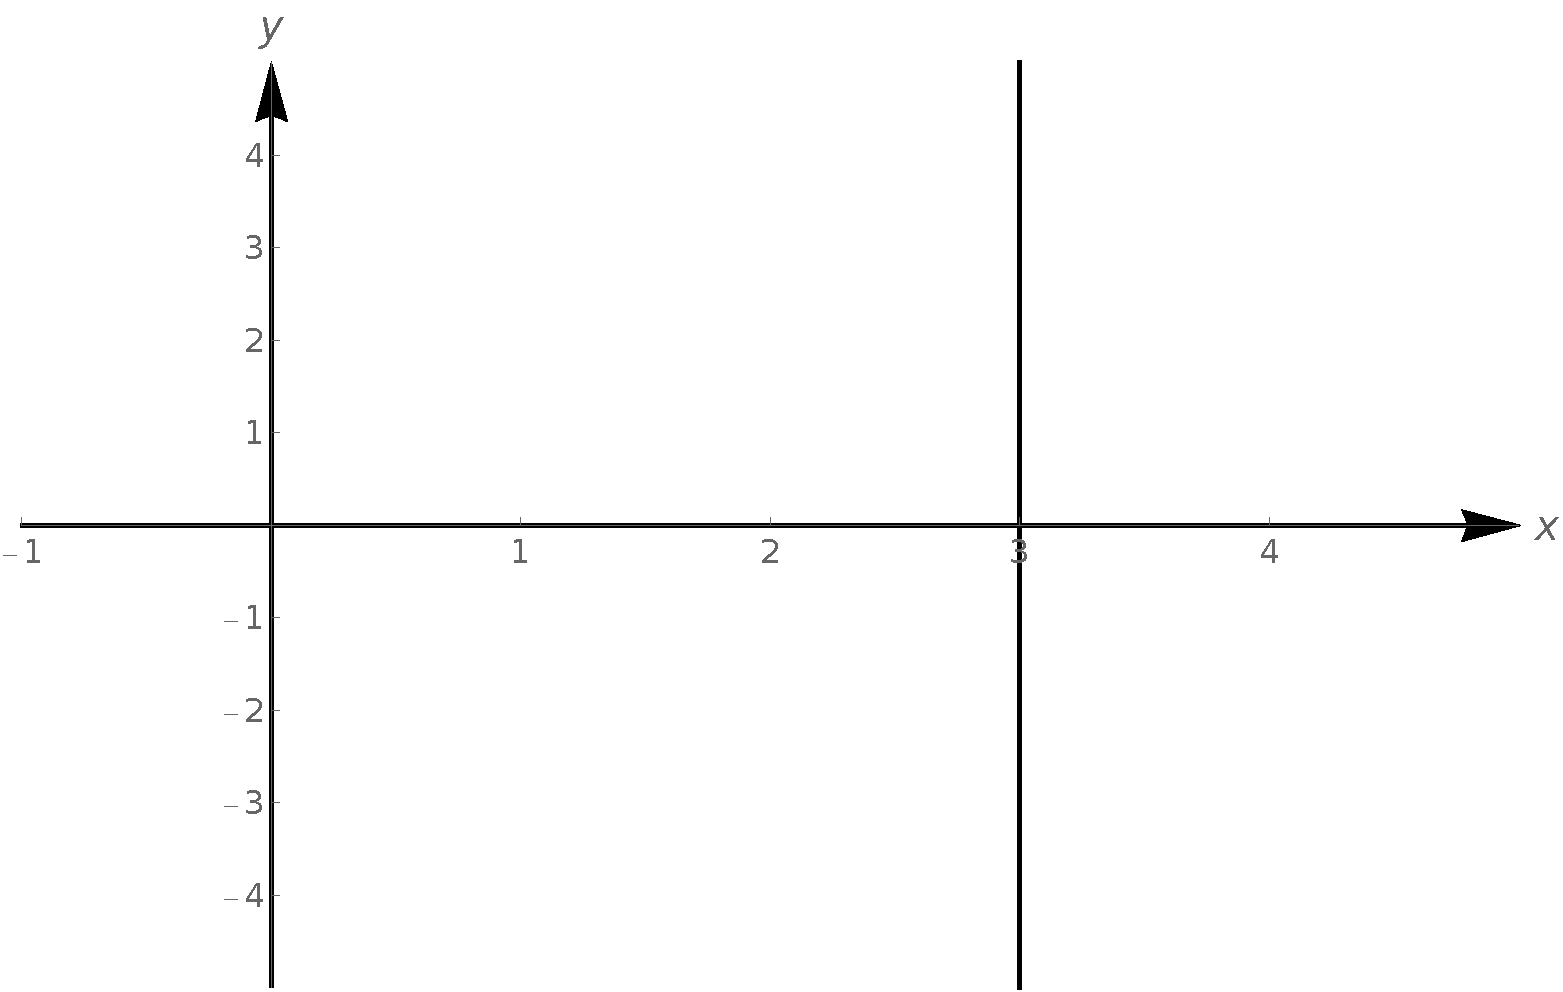
\includegraphics[width=0.4\textwidth]{fig_functions_3c}}
}
\caption{Graphs of different relations.} 
\end{figure}
\fi

\end{example}


The relation $C$ in the previous example lead us to our final way to describe relations: \textbf{algebraically} (\textit{algebra\"isch}). We can more succinctly describe the points in $C$ as those points which satisfy the equation $x = 3$.  Let us now study the graphs of equations in a more general setting. For that purpose, we rely on the so-called fundamental graphing principle.\index{fundamental graphing principle}
\index{algebraic notation}\index[aut]{algebra\"ische notatie}


\begin{definition}[Fundamental graphing principle]
The graph of an equation is the set of points which satisfy the equation.  %That is, a point $(x,y)$ is on the graph of an equation if and only if $x$ and $y$ satisfy the equation.
\end{definition}

It is at this point that we gain some insight into the word `relation'.  If the equation to be graphed contains both $x$ and $y$, then the equation itself is what is relating the two variables.  For instance, in the next example, we consider the  graph of the equation $x^2+y^3=1$ by graphing the relation $R = \{ (x,y) \, | \, x^2+y^3 = 1\}$.  \ifvc The points $(x,y)$ we graph belong to the relation $R$ and are related by the equation  $x^2+y^3 = 1$, since it is those pairs of $x$ and $y$ which make the equation true.\fi

\begin{example}
\label{examplerelation}
Graph the equation $x^2 + y^3 = 1$.

\xhrulefill{gray}{2.5pt}Solution \xhrulefill{gray}{2.5pt}

To  efficiently generate points on the graph of this equation, we first solve this equation for $y$:

\allowdisplaybreaks
\[ \begin{array}{rrclr} 
&    x^2 + y^3 & = & 1 & \\ 
\Leftrightarrow &          y^3 & = & 1 - x^2 & \\
\Leftrightarrow &\sqrt[3]{y^3} & = & \sqrt[3]{1 - x^2} & \\
\Leftrightarrow &            y & = & \sqrt[3]{1 - x^2}\,. & \\ 
            \end{array} \]

We now substitute a value in for $x$, determine the corresponding value $y$, and plot the resulting point $(x,y)$ in the Cartesian coordinate plane. We first generate a table of points which are on the graph of the equation.  These points are then plotted in the plane as shown below.

\begin{minipage}[c]{0.45\textwidth}
\begin{center}
\renewcommand{\arraystretch}{1.5}%
\begin{tabular}{c|c}  
	$x$&$y$ \\ \hline\hline
	$-3$&$ -2$ \\  
	$-2$&$-\sqrt[3]{3}$ \\  
	$ -1$&$ 0$ \\  
	$ 0 $&$ 1$ \\  
	$ 1$&$ 0$ \\  
	$2$&$-\sqrt[3]{3}$ \\  
	$3$&$ -2$ \\  
\end{tabular}
\end{center}
\end{minipage}
\begin{minipage}[c]{0.45\textwidth}
	\begin{center}
			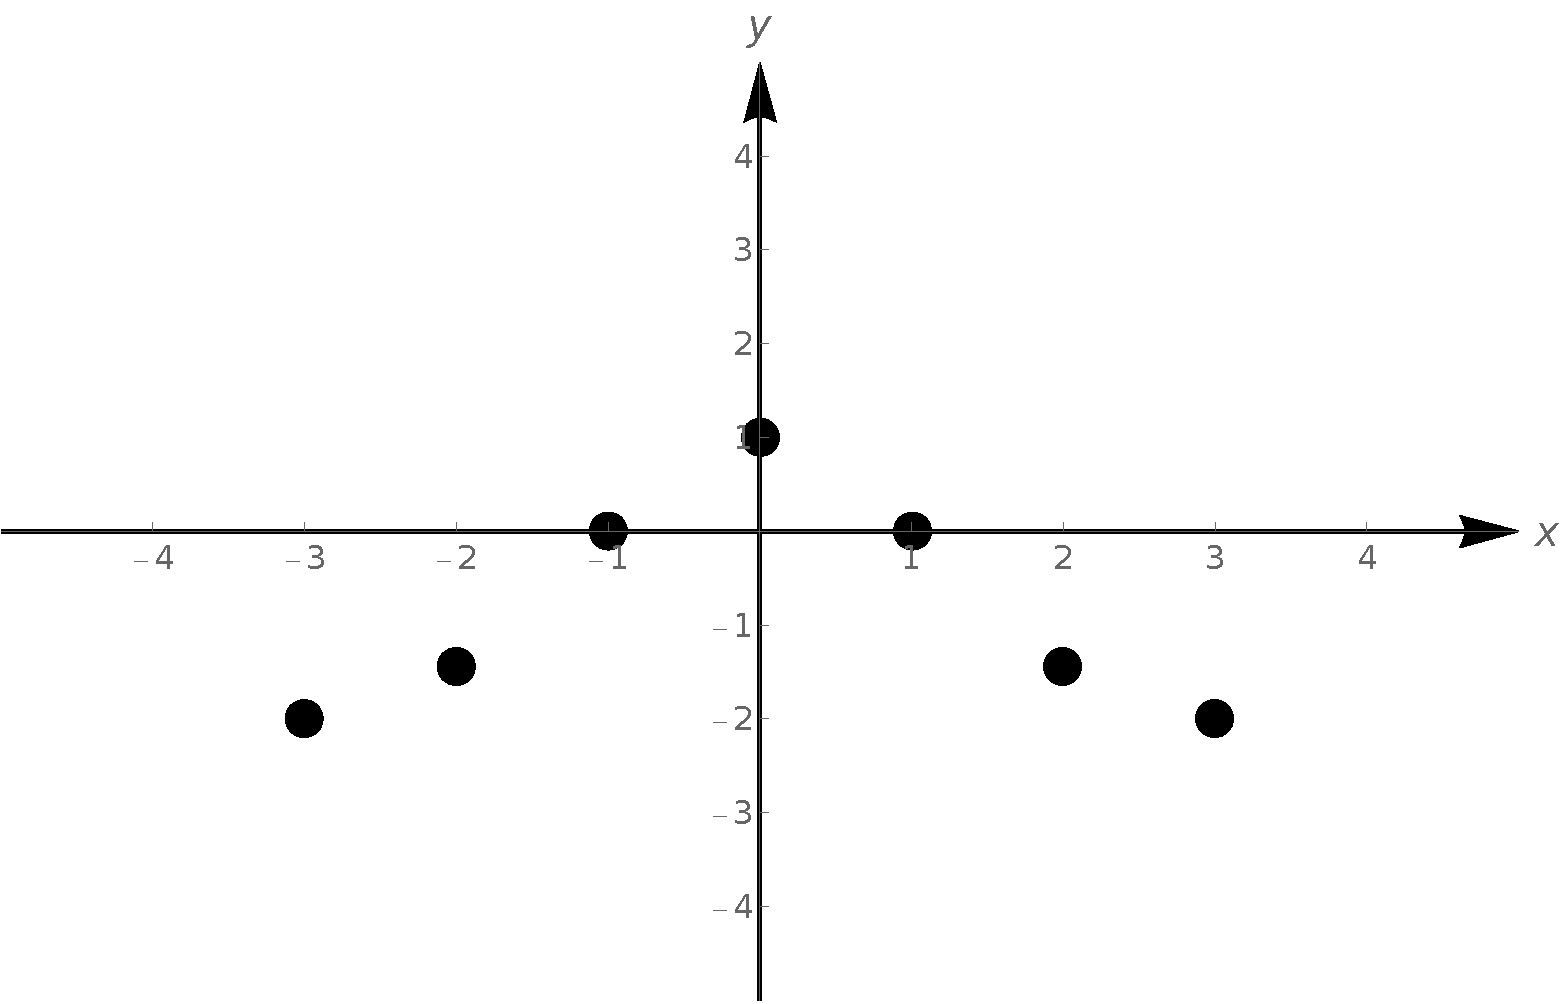
\includegraphics[width=0.95\textwidth]{fig_functions_4}
	\end{center}
\end{minipage}

  
\ifcourse
\ifmathematica
Alternatively, we can construct a graph of this equation in Mathematica using the built-in function \lstinline{ContourPlot}:
\begin{mdframed}[default,backgroundcolor=gray!40,roundcorner=8pt]
\begin{mmaCell}[morefunctionlocal={x, y}]{Input}
  ContourPlot[x^2+y^3==1,\{x,-5,5\},\{y,-5,5\}]

\end{mmaCell}


\begin{mmaCell}[moregraphics={moreig={scale=.4}}]{Output}
	 \mmaGraphics{fig_functions_5}
\end{mmaCell}
\end{mdframed}

Of course, we should add frame labels to this plot, which can be done as follows.
\begin{mdframed}[default,backgroundcolor=gray!40,roundcorner=8pt]
\begin{mmaCell}[morefunctionlocal={x, y}]{Input}
   ContourPlot[x^2+y^3==1,\{x,-5,5\},\{y,-5,5\}, FrameLabel \(\pmb{\to}\)\{"x","y"\}]

\end{mmaCell}


\begin{mmaCell}[moregraphics={moreig={scale=.4}}]{Output}
	 \mmaGraphics{fig_functions_6}
\end{mmaCell}
\end{mdframed}
\fi
\fi
\ifpython
Alternatively, we can construct a graph of this equation in Python using the built-in function \lstinline{plot}:
\begin{pyin}
from sympy import plot_implicit, symbols, Eq, And

x, y = symbols('x y')
p1 = plot(Eq(x**2 + y**3, 1))
\end{pyin}

\begin{pyout}
|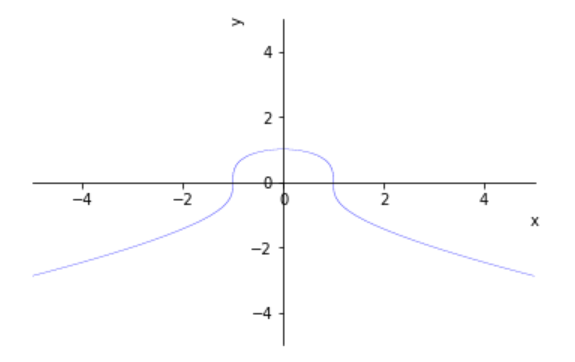
\includegraphics[width=0.5\textwidth]{fig_functions_6_Python}|
\end{pyout}
\fi
\end{example}




The places where the graph of an equation crosses or touches the axes are called the \textbf{intercepts} (\textit{intercept}). \index{intercept}\index[aut]{intercept}  \ifvc The $x$-intercepts can be found by setting $y = 0$ in the equation, while $y$-intercepts are found by setting $x = 0$ in the equation.  In Example~\ref{examplerelation} the graph had two $x$-intercepts, $(-1,0)$ and $(1,0)$, and one $y$-intercept, $(0,1)$. \fi 

Another fact which you may have noticed about the graph in Example~\ref{examplerelation} is that it seems to be symmetric about the $y$-axis.  To actually prove this analytically, we assume $(x,y)$ is a generic point on the graph of the equation. That is, we assume  $x^2 + y^3 = 1$ is true. To show that the graph as a whole is symmetric about the $y$-axis, we need to show that $(-x,y)$ satisfies the equation $x^2 + y^3 = 1$, too.  Substituting $(-x,y)$ into the equation gives

\setlength{\extrarowheight}{2pt}

\[ \begin{array}{rrclr}   
&(-x)^2+(y)^3 & \stackrel{?}{=} & 1 & \\
\Leftrightarrow &  x^2 + y^3 & \stackrel{\checkmark}{=} & 1. & \\ 
   \end{array} \]
   
Since we are assuming that the original equation $x^2 + y^3 = 1$ is true, we have shown that $(-x, y)$ satisfies the equation and hence is on the graph.  In this way, we can check whether the graph of a given equation possesses any of the symmetries introduced in Section~\ref{CartesianPlane}.  



\begin{itemize}
	
	\item About the $y$-axis: substitute $(-x,y)$ into the equation and verify whether or not the result is equivalent to the original equation.
	
	\item About the $x$-axis: substitute $(x,-y)$ into the equation   and verify whether or not the result is equivalent to the original equation.
	
	\item About the origin: substitute $(-x,-y)$ into the equation and verify whether or not the result is equivalent to the original equation.
	
\end{itemize}


\ifcalculus
Intercepts and symmetry are two tools which can help us sketch the graph of an equation analytically, as demonstrated in the next example.


\begin{example}
	Find the $x$- and $y$-intercepts (if any) of the graph of $(x-2)^2 + y^2 = 1$. Test for symmetry.  Plot additional points as needed to complete the graph.
	
	\xhrulefill{gray}{2.5pt}Solution \xhrulefill{gray}{2.5pt}
	
	To look for $x$-intercepts, we set $y=0$ and solve
	
	\[ \begin{array}{rrclr}   
	
	&(x-2)^2 + 0^2 & = & 1 & \\ 
	\Leftrightarrow &\sqrt{(x-2)^2} & = & \sqrt{1} & \\
	\Leftrightarrow &x - 2 & = & \pm 1 & \\
	\Leftrightarrow &x  = 3 & \wedge & x  =  1. & \\
	
	\end{array} \]
	
	We get two answers for $x$ which correspond to two $x$-intercepts:  $(1,0)$ and $(3,0)$.    Turning our attention to $y$-intercepts, we set $x=0$ and solve
	
	\[ \begin{array}{rrclr}   
	
	&(0-2)^2 + y^2 & = & 1 & \\ 
	\Leftrightarrow&4 + y^2 & = & 1 & \\
	\Leftrightarrow&y^2 & = & -3. & \\
	
	\end{array} \]
	Consequently, the graph has no (real-valued!) $y$-intercepts.
	
	
	Moving along to symmetry, we can immediately dismiss the possibility that the graph is symmetric about the $y$-axis or the origin.  If the graph possessed either of these symmetries, then the fact that $(1,0)$ is on the graph would mean $(-1,0)$ would have to be on the graph. The only symmetry left to test is symmetry about the $x$-axis.   To that end, we substitute $(x,-y)$ into the equation and simplify
	
	\[ \begin{array}{rrclr}   
	&(x-2)^2 + (-y)^2 & = & 1 & \\ 
	\Leftrightarrow&(x-2)^2 + y^2 & = & 1 .& \\
	\end{array} \]
	
	Since we have obtained our original equation, the graph is symmetric about the $x$-axis. Proceeding as we did in the Example~\ref{examplerelation}, we obtain the graph shown in Figure~\ref{fig_functions_7}.
	
	
	\begin{figure}[H]
		\begin{center}
			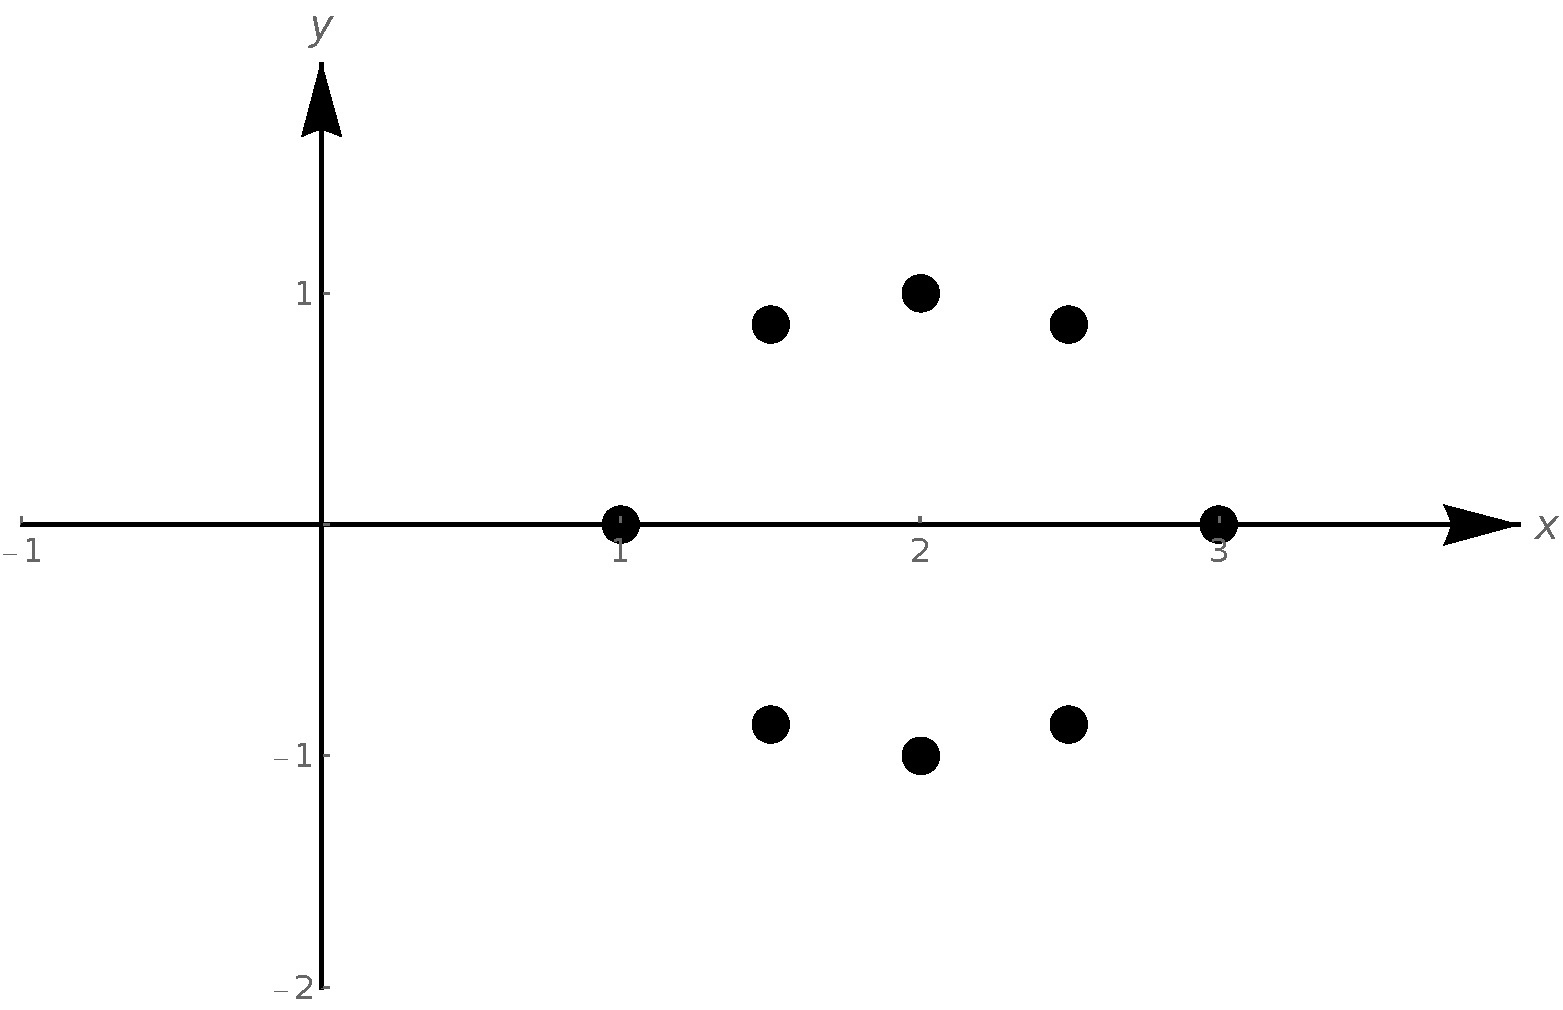
\includegraphics[width=0.5\textwidth]{fig_functions_7}
			\caption{Graph of the equation $(x-2)^2 + y^2 = 1$.}
			\label{fig_functions_7}
		\end{center}
	\end{figure}
	
\end{example}
\fi


\ifvc
\begin{itemize}

\item About the $y$-axis: substitute $(-x,y)$ into the equation and verify whether or not the result is equivalent to the original equation.

\item About the $x$-axis: substitute $(x,-y)$ into the equation   and verify whether or not the result is equivalent to the original equation.

\item About the origin: substitute $(-x,-y)$ into the equation and verify whether or not the result is equivalent to the original equation.

\end{itemize}

Intercepts and symmetry are two tools which can help us sketch the graph of an equation analytically, as demonstrated in the next example.


\begin{example}
 Find the $x$- and $y$-intercepts (if any) of the graph of $(x-2)^2 + y^2 = 1$. Test for symmetry.  Plot additional points as needed to complete the graph.

\xhrulefill{gray}{2.5pt}Solution \xhrulefill{gray}{2.5pt}

To look for $x$-intercepts, we set $y=0$ and solve

\[ \begin{array}{rrclr}   

&(x-2)^2 + 0^2 & = & 1 & \\ 
\Leftrightarrow &\sqrt{(x-2)^2} & = & \sqrt{1} & \\
\Leftrightarrow &x - 2 & = & \pm 1 & \\
\Leftrightarrow &x  = 3 & \wedge & x  =  1. & \\

\end{array} \]

We get two answers for $x$ which correspond to two $x$-intercepts:  $(1,0)$ and $(3,0)$.    Turning our attention to $y$-intercepts, we set $x=0$ and solve

\[ \begin{array}{rrclr}   

&(0-2)^2 + y^2 & = & 1 & \\ 
\Leftrightarrow&4 + y^2 & = & 1 & \\
\Leftrightarrow&y^2 & = & -3. & \\

\end{array} \]
Consequently, the graph has no (real-valued!) $y$-intercepts.


Moving along to symmetry, we can immediately dismiss the possibility that the graph is symmetric about the $y$-axis or the origin.  If the graph possessed either of these symmetries, then the fact that $(1,0)$ is on the graph would mean $(-1,0)$ would have to be on the graph. The only symmetry left to test is symmetry about the $x$-axis.   To that end, we substitute $(x,-y)$ into the equation and simplify

\[ \begin{array}{rrclr}   
&(x-2)^2 + (-y)^2 & = & 1 & \\ 
\Leftrightarrow&(x-2)^2 + y^2 & = & 1 .& \\
\end{array} \]

Since we have obtained our original equation, the graph is symmetric about the $x$-axis. Proceeding as we did in the Example~\ref{examplerelation}, we obtain the graph shown in Figure~\ref{fig_functions_7}.


\begin{figure}[H]
	\begin{center}
			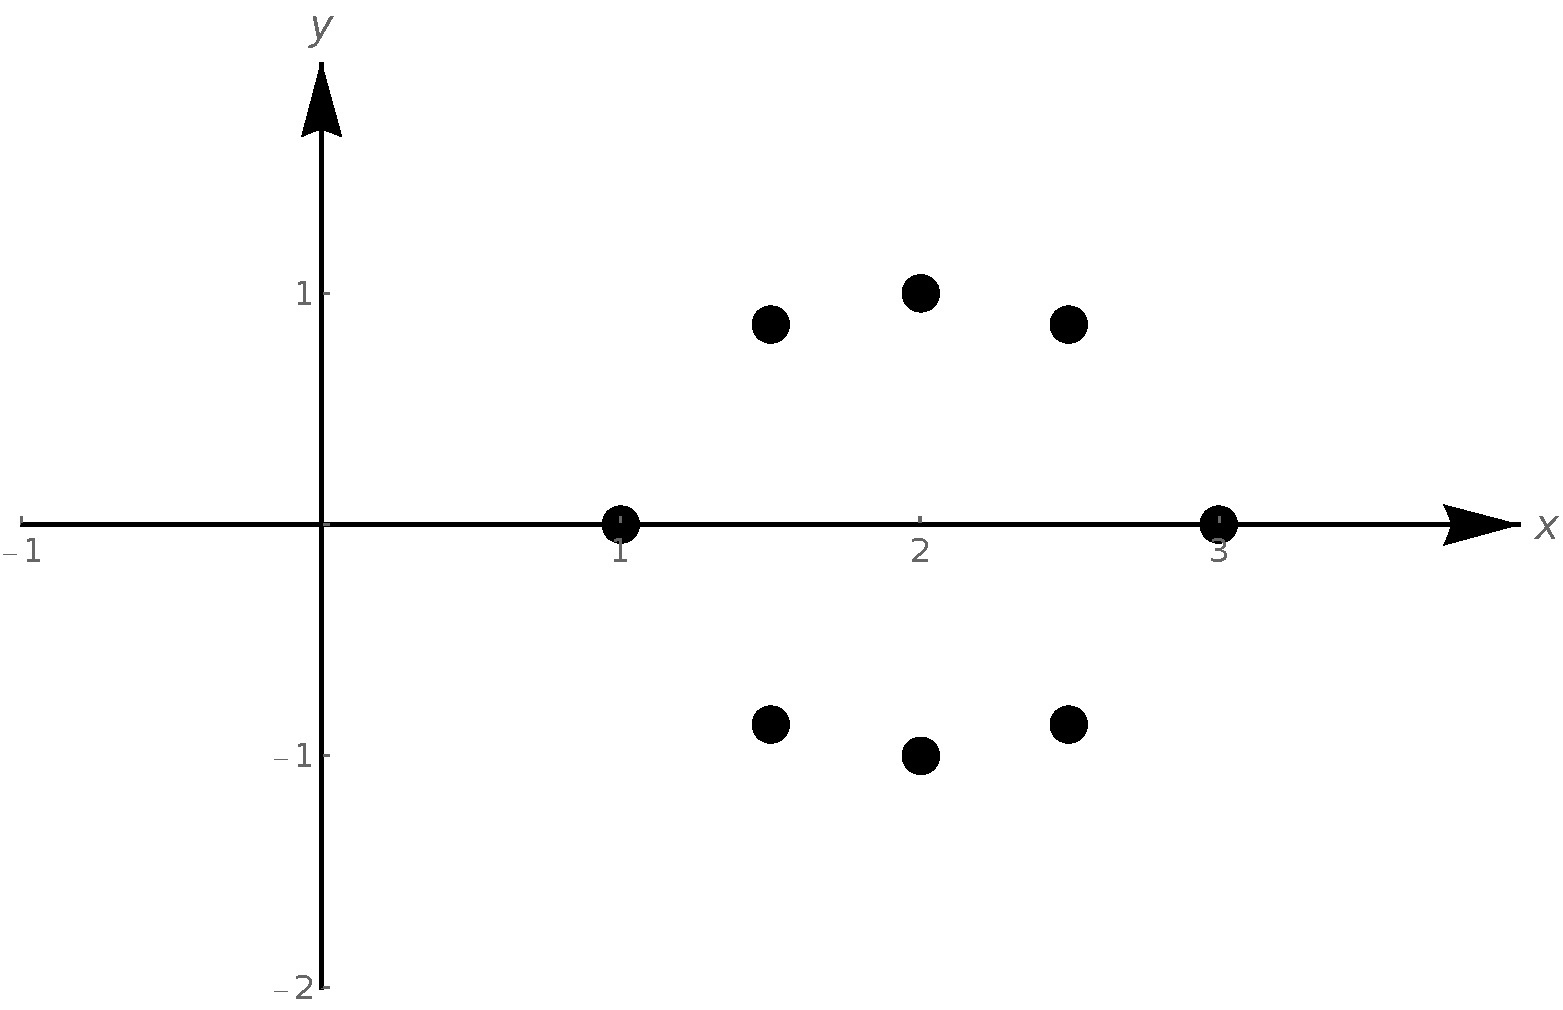
\includegraphics[width=0.5\textwidth]{fig_functions_7}
	\caption{Graph of the equation $(x-2)^2 + y^2 = 1$.}
	\label{fig_functions_7}
	\end{center}
\end{figure}

\end{example}
\fi

\subsection{Functions in $\mathbb{R}$}\label{functies_R}
\subsubsection{Definition}

\begin{definition}[Function]
\label{def_function}

A relation in which each $x$-coordinate in $\mathbb{R}$ is matched with at most only one $y$-coordinate is said to describe $y$ as a \textbf{function} (\textit{functie}) of $x$. A function $f$ that maps $x$ to $y$ is denoted as
$$
f: x\mapsto f(x)\,,
$$
with  $y = f ( x )$.
\end{definition}
\index{function}\index[aut]{functie}
The notation $y = f ( x )$ (read: $y$ equals $f$ of $x$) means that the pair $(x, y)$ belongs to the set of pairs defining the function $f$. $x$ is called the \textbf{argument} or \textbf{input} (\textit{input}) of the function $f$ and $f (x)$ is called the \textbf{value} taken by the function when evaluated at a point $x$, or its \textbf{output} (\textit{output}) or \textbf{image}. In the framework of applications, $x$ is often called the \textbf{independent variable} (\textit{onafhankelijke veranderlijke}), while $y$ is called the \textbf{dependent variable} (\textit{afhankelijke veranderlijke}). 
Loosely speaking, a function may be envisaged as a black box that returns for each input a corresponding output (Figure~\ref{fig_functions_8}). 
\index{argument}\index[aut]{argument}
\index{input}\index[aut]{input} 
\index{output}\index[aut]{output}
\index{image}\index[aut]{beeld}
\index{dependent variable}\index[aut]{afhankelijke veranderlijke}
\index{independent variable}\index[aut]{onafhankelijke veranderlijke}

\begin{figure}[H]
	\begin{center}
	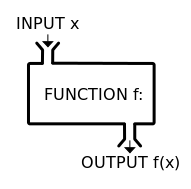
\includegraphics[width=0.25\textwidth]{fig_functions_8}
	\caption{Describing a function as a black box.}
	\label{fig_functions_8}
	\end{center}
\end{figure}




To (graphically) determine whether or not a relation is function, we can use the following theorem, which is an immediate consequence of Definition~\ref{def_function}. 

\begin{theorem}[Vertical line test]
\label{VLT}
A set of points in the plane represents $y$ as a function of $x$ if and only if no two points lie on the same vertical line.
\end{theorem}
\ifanalysis
\begin{proof}
This is a direct consequence of Definition~\ref{def_function}
\end{proof}
\fi
\ifanalysis In other words, a relation $R$ constitutes a function if and only if every line parallel to the $y$-axis intersects the graph of $R$ in at most one point. \fi 


\begin{example}
Determine graphically which of the following relations actually represents a function.

\begin{figure}[H]
\centering
%\raisebox{0.5cm}{
\centerline{
\subfigure[Graph of relation $A$ \label{fig_functions_9a}]{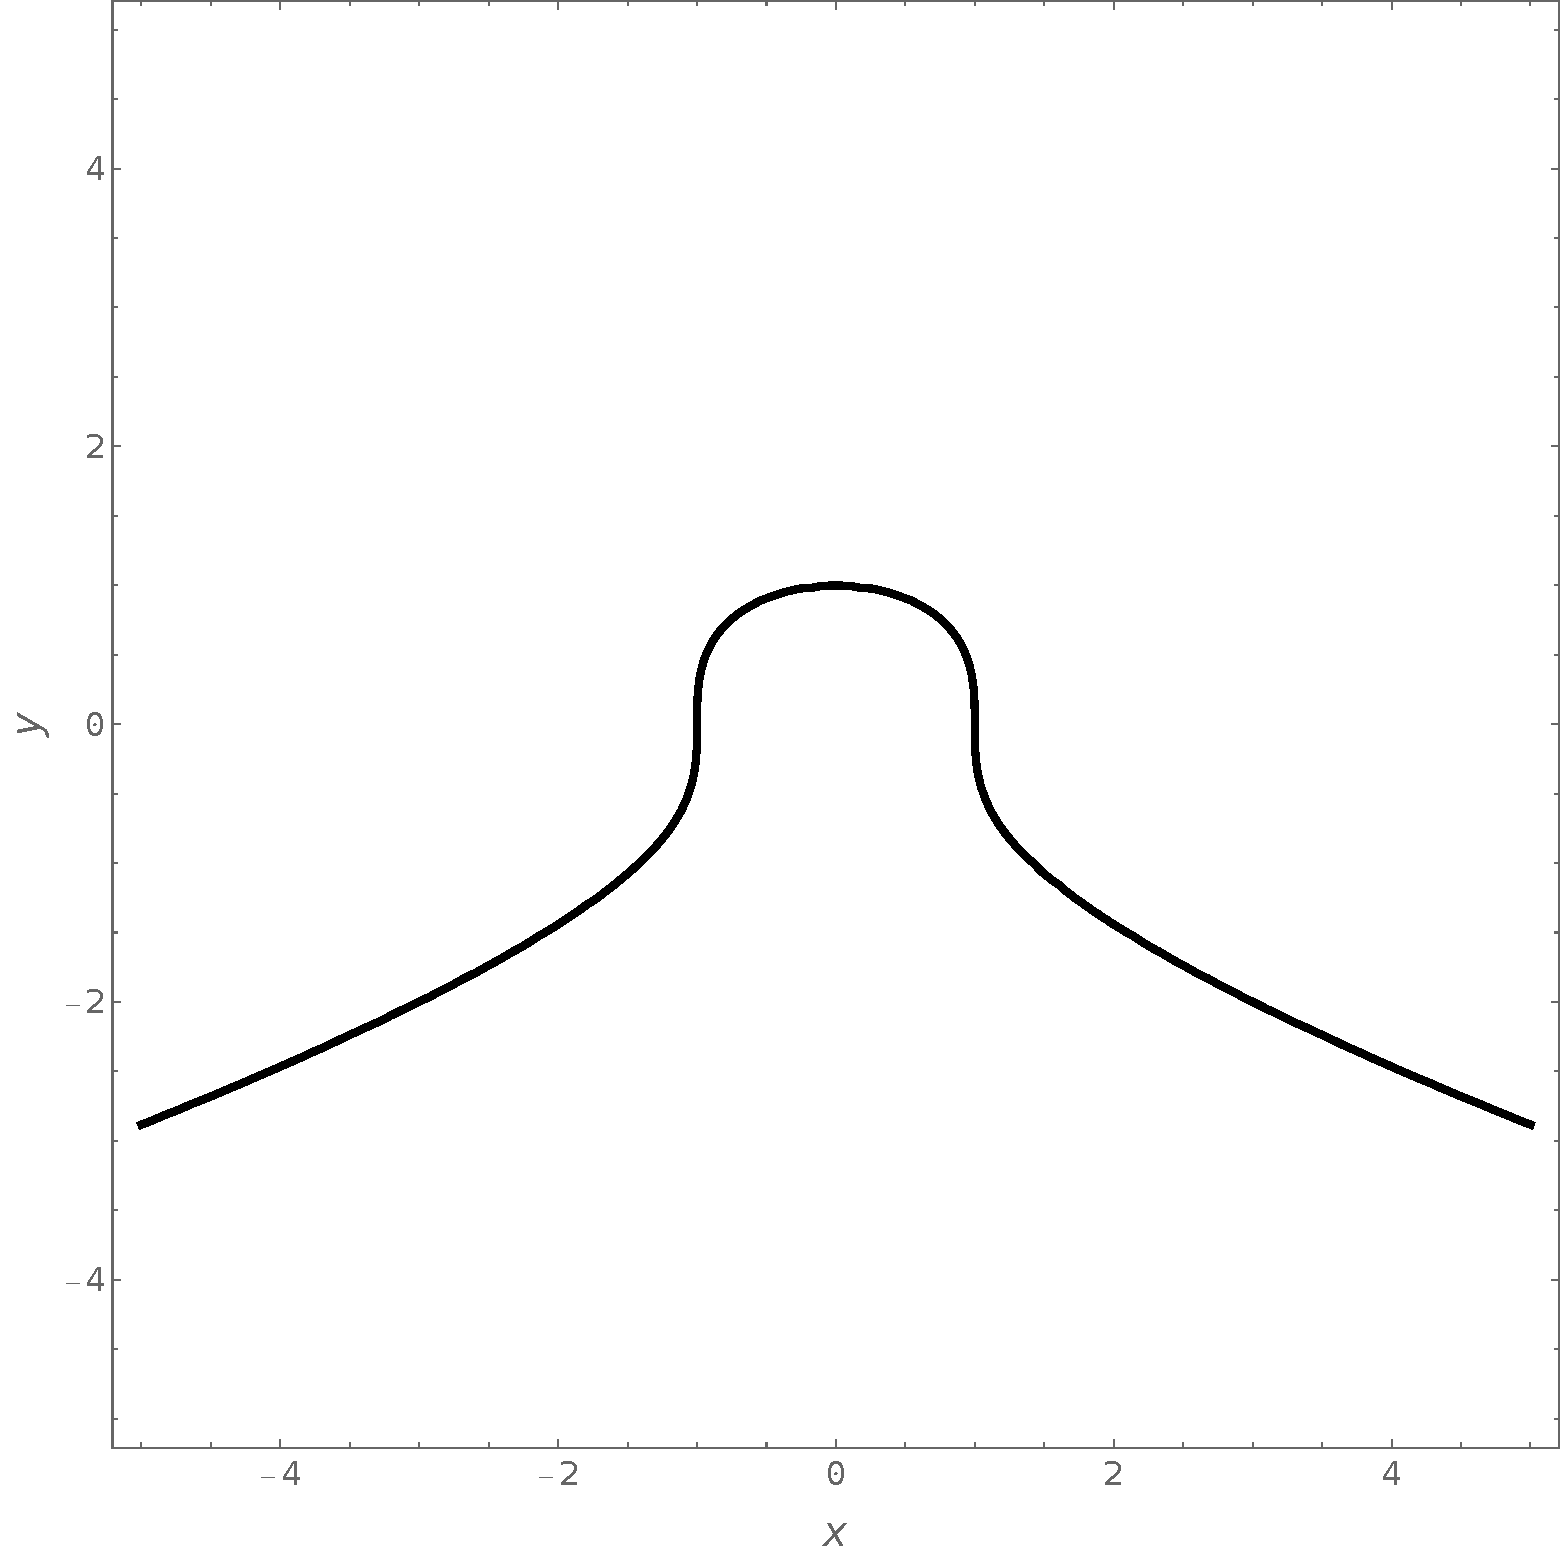
\includegraphics[width=0.35\textwidth]{fig_functions_9a}}
\hspace{0.1cm}
\subfigure[Graph of relation $B$ \label{fig_functions_9b}]{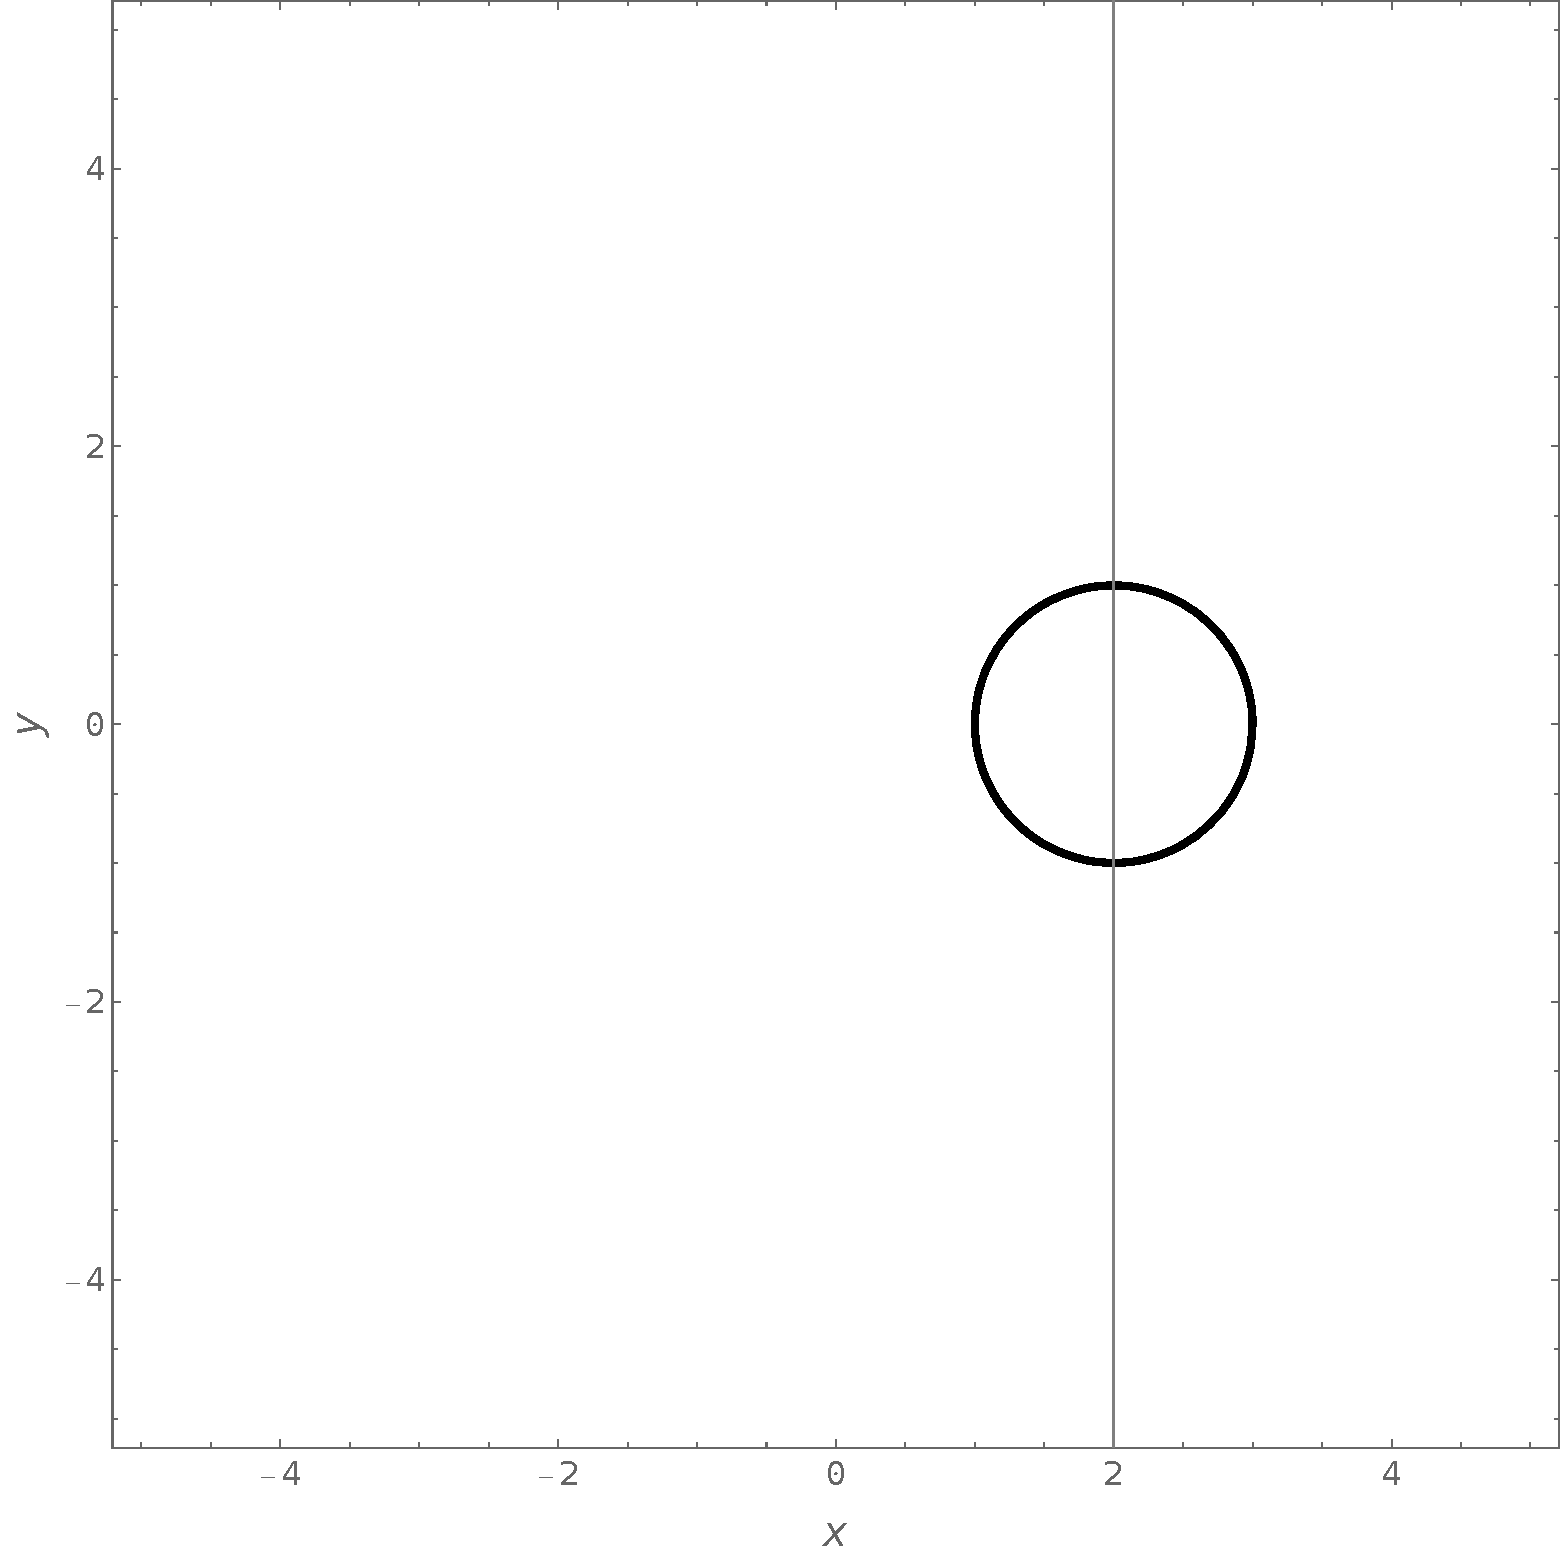
\includegraphics[width=0.35\textwidth]{fig_functions_9b}}
}
\centerline{
\subfigure[Graph of relation $C$ \label{fig_functions_9c}]{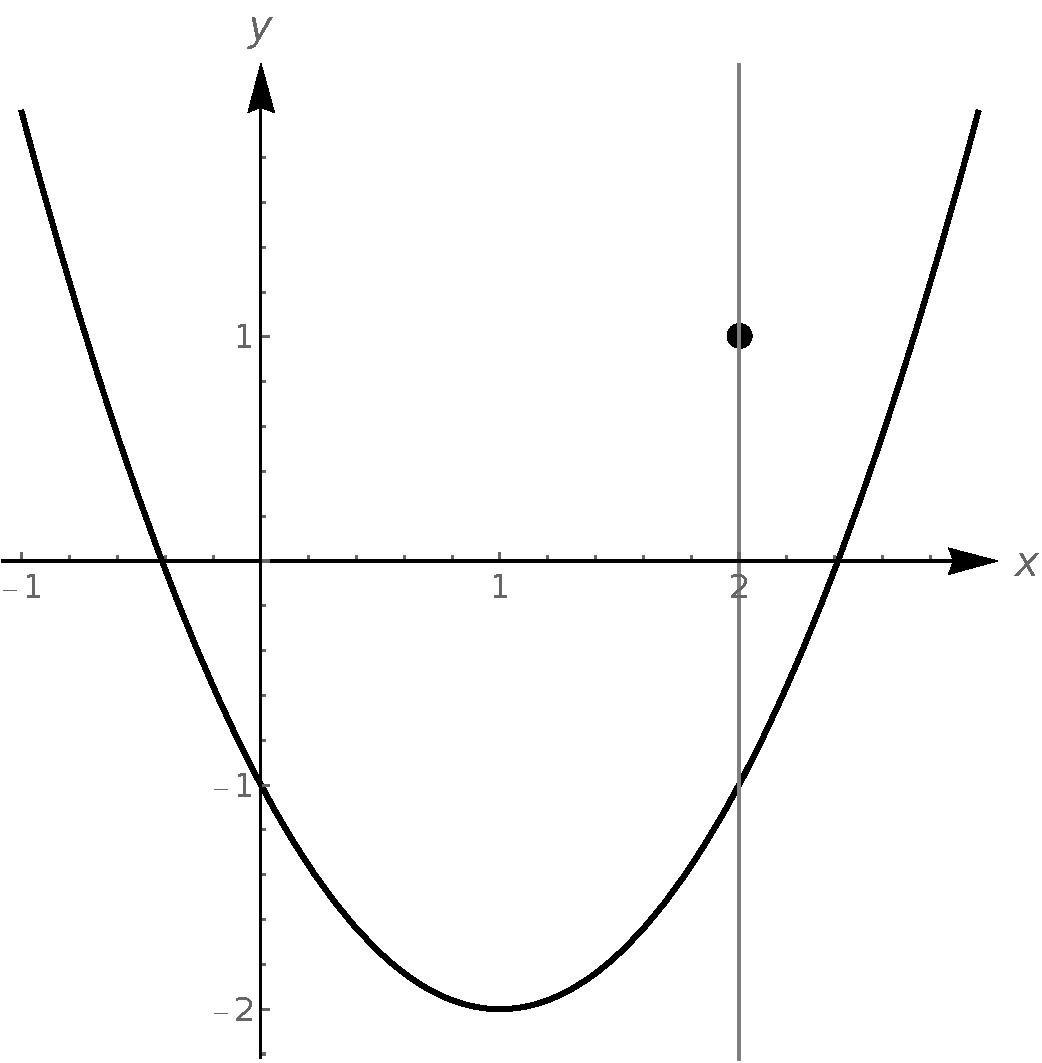
\includegraphics[width=0.35\textwidth]{fig_functions_9c}}
\hspace{0.1cm}
\subfigure[Graph of relation $D$ \label{fig_functions_9d}]{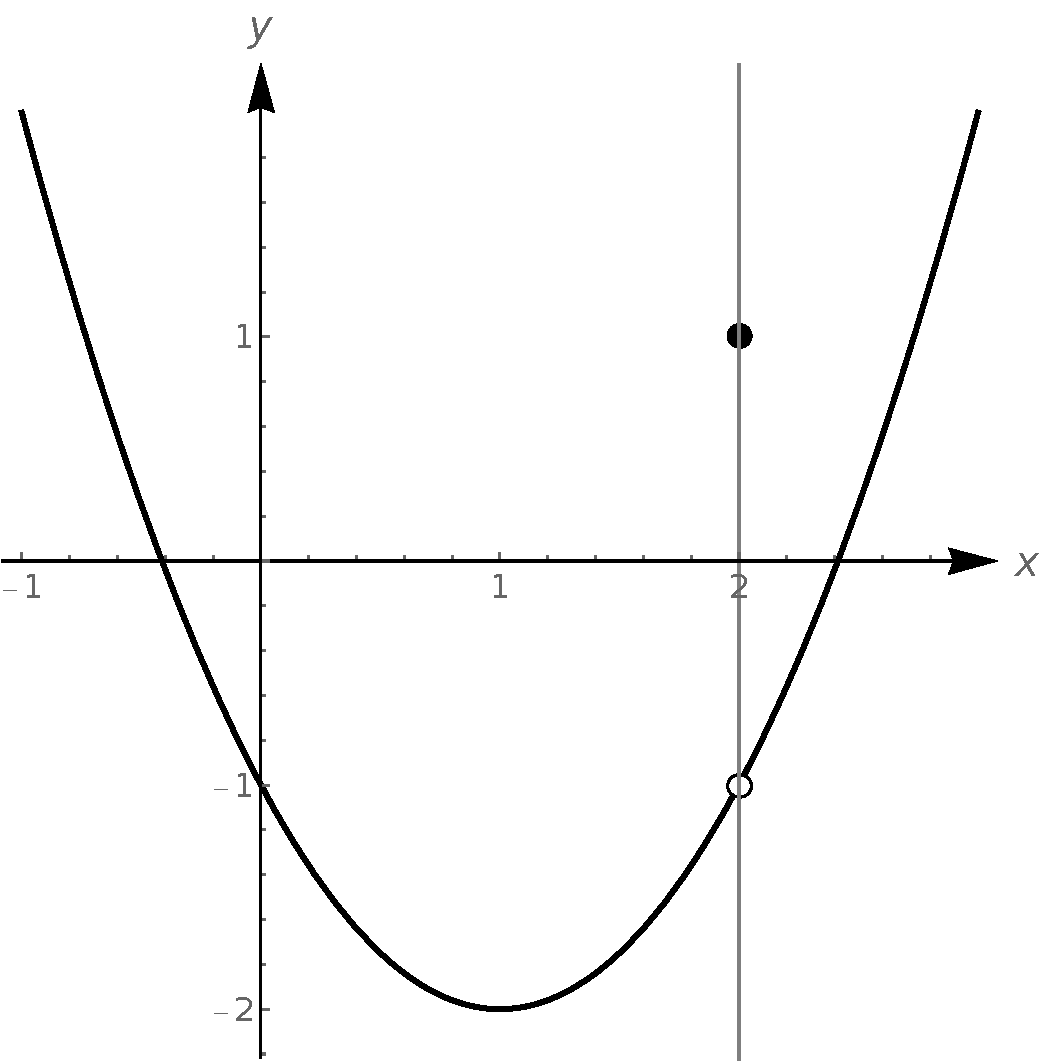
\includegraphics[width=0.35\textwidth]{fig_functions_9d}}
}

\end{figure}

\xhrulefill{gray}{2.5pt}Solution \xhrulefill{gray}{2.5pt}

\begin{enumerate}
\item [(a)]   In the graph of $A$, every vertical line crosses the graph at most once, so $A$ does represent $y$ as a function of $x$.
\item [(b)] Looking at the graph of $B$, we can easily imagine a vertical line crossing the graph more than once.  Hence, $B$ does not represent $y$ as a function of $x$.  
\item [(c)]  In $C$, there is a point on the curve with $x$-coordinate 2 just below $(2,1)$, which means that both $(2,1)$ and this point on the curve lie on the vertical line $x=2$.  Hence, the graph of  $C$ fails the vertical line test, so $y$ is not a function of $x$ here. 
\item [(d)] In $D$ notice that the point with $x$-coordinate 2 on the curve has been omitted, leaving an open circle there.  Hence, the vertical line $x=2$ crosses the graph of $D$ only at the point $(2,1)$.  Indeed, any vertical line will cross the graph at most once, so we have that the graph of $D$ passes the vertical line test.  Thus it describes $y$ as a function of $x$.
\end{enumerate}
\end{example}

Finally, it is important to note that a function for which the dependent variable can be written explicitly in terms of the independent variable, i.e.\ as $y=f(x)$, is called an \textbf{explicit function} (\textit{expliciete functie}). On the other hand, if the function is defined by
$$
F(x,y)=0\,,
$$
which does not contain $y$ explicitly at one side of the equation, it is called an \textbf{implicit function} (\textit{impli\-ciete functie}). For instance, 
$$
x^2+y^2-4=0
$$
constitutes an implicit function, which defines two explicit functions, namely
$$
y=\sqrt{4-x^2},\qquad\mbox{and} \qquad y=-\sqrt{4-x^2}\,.
$$
\index{implicit function}\index[aut]{impliciete functie}\index{explicit function}\index[aut]{expliciete functie}\index{function ! implicit}\index[aut]{functie ! impliciet}\index{function ! explicit}\index[aut]{functie ! expliciet}

\subsubsection{Function graphs}
It is often useful to draw the graph\index{graph}\index[aut]{grafiek} of a function for getting a global view of its properties. Formally, we define the graph of a function as follows. 
\begin{definition}[Fundamental graphing principle for functions]
The graph $G$ of a function $f$ is the set of points which satisfy the equation $y=f(x)$. More formally, 
$$
G=\left\{(x,f(x))\mid x \in \mathbb{R} \wedge y=f(x)\right\}\,.
$$
\end{definition}
The $x$-coordinates of the $x$-intercepts of the graph of $y=f(x)$ can be found by solving $f(x) = 0$.  For this reason, they are called the \index{function ! zero}\index{functie ! nulpunt}\textbf{zeros} (\textit{nulpunt}) of $f$.


\subsubsection{Domain, codomain and range}
When defining a function $f$ as
$$
f: x\mapsto f(x)\,,
$$
\ifcourse
	\checkoddpage
\marginpar{\ifoddpage\hspace*{-1.5cm}\else\hspace*{0.25cm}\fi
\includegraphics[width=0.075\textwidth]{youtube}\\
\ifoddpage\hspace*{-1.75cm}\else\hspace*{0.1cm}\fi
\qrcode[height=1.75cm]{https://youtu.be/BQMyeQOLvpg}
%\includegraphics[width=0.1\textwidth]{codomein}
}
\fi
we not only need to specify how $f$ maps an argument $x$ to its image $y$, but also the sets to which $x$ and $y=f(x)$ belong. In other words, we need to specify what are the possible in- and outputs of our black box (Figure~\ref{fig_functions_8}). We call the set of possible inputs the \textbf{domain} (\textit{domein}) of the function, denoted as $\dom{\;f}$. The set of possible outputs is called the \textbf{codomain} (\textit{codomein}). Suppose $X$ is the domain of a function $f$ and $Y$ is its codomain, then we can define this function using arrow notation to make explicit the domain and codomain:
\index{domain}\index[aut]{domein}
\index{codomain}\index[aut]{codomein}
$$
f:X\to Y\,,
$$
which should be read as $f$ maps domain $X$ to codomain $Y$. The set to which $f$ actually maps the domain, is called the \textbf{range} (\textit{bereik}) or \textbf{image} (\textit{beeld}) of $f$, denoted by $\im{\;f}$. The range is thus defined as
\index{range}\index[aut]{bereik}
$$
\im{\;f} = \left\{y=f(x)\mid x\in X \wedge y\in Y \right\}\,.
$$
These concepts are illustrated in Figure~\ref{fig_functions_10}. The difference between range and codomain may seem subtle, but can be very important, as will be shown in Example~\ref{example_domain_codomain_range}.

\begin{figure}[h!]
	\begin{center}
	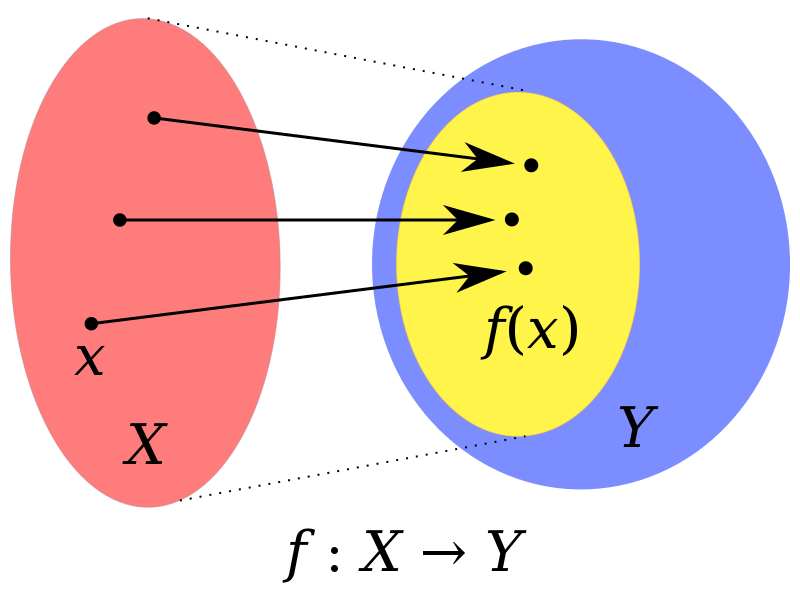
\includegraphics[width=0.4\textwidth]{figures/Functions/fig_functions_10.png}
	\caption{The domain $X$, codomain $Y$ and range $\left\{f(x)\mid x\in X\right\}$ of a function $f$.}
	\label{fig_functions_10}
	\end{center}
\end{figure}

Throughout this course we will focus on so-called \textbf{real functions} (\textit{re\"ele functie}), which are real-valued functions of a real variable. Such functions can be written as \index{real function}\index[aut]{re\"ele functie}
$$
f:\mathbb{R}\to\mathbb{R}\quad:\quad x\mapsto f(x)\,.
$$


\ifvc
To determine the domain and range of a function, we need to determine which $x$ and $y$-values occur as coordinates of points on the given graph.  To find the domain graphically, it may be helpful to imagine collapsing the curve to the $x$-axis and determining the portion of the $x$-axis that gets covered. The resulting interval on the $x$-axis represents the domain of $f$. This is called \textbf{projecting} (\textit{projectie}) the curve to the $x$-axis. To determine the range of $f$, we project the curve to the $y$-axis. \index{projection}\index[aut]{projectie}

\begin{example}
Determine the domain and range of the function $f$ whose graph is given below.
	\begin{center}
			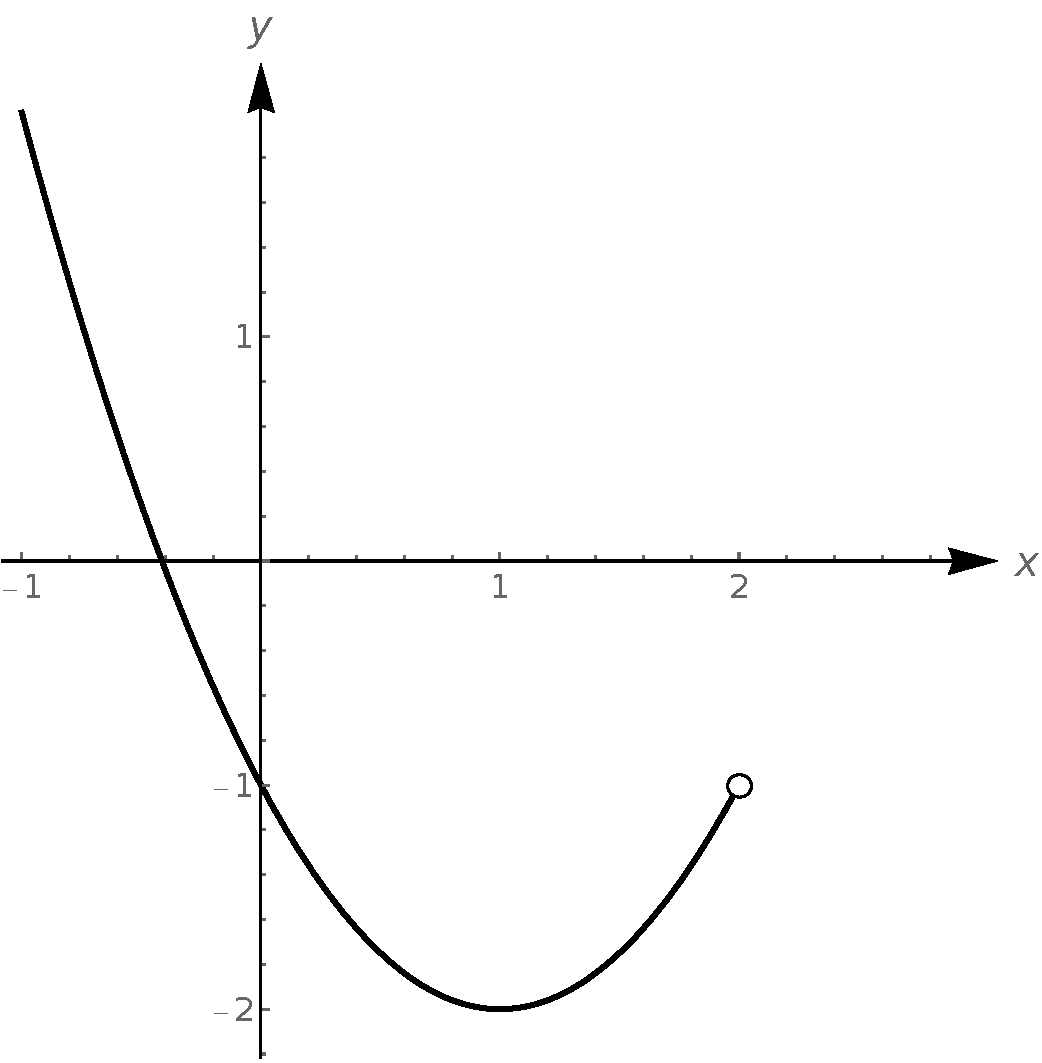
\includegraphics[width=0.5\textwidth]{fig_functions_11}
	\end{center}

\pagebreak 
\xhrulefill{gray}{2.5pt}Solution \xhrulefill{gray}{2.5pt}
	
   First note that the graph continues to curve upwards
   to the left forever more; and note the open circle at $(2,-1)$ that indicates that the point $(2,-1)$ is not on the graph, but all points on the curve leading up to that point are. We see  that if we project the graph of $f$ to the $x$-axis, we get all real numbers less than $2$.  Using interval notation, we write the domain of $f$ as $\left.\right]-\infty, 2\left.\right[$. Note that even though there is an open circle at $(2,-1)$, we still include the $y$-value of $-1$ in our range, since the point $(0,-1)$ is on the graph of $f$.  We see that the range of $f$ is all real numbers greater than or equal to $-2$, or, in interval notation,  $\left.\right]-2,+\infty]$.
\end{example}
\fi

In most cases, we can relatively easily determine the domain, codomain and range of a function $f$ by investigating the formula defining it.  Doing so, we sometimes run into functions whose domain consists of two ore more consecutive open intervals, such as for  $$f(x)=\frac{1}{x}\,,$$ for  which $\text{dom}\,f=\mathbb{R}\setminus\{0\}=]-\infty,0[\,\cup\, ]0,+\infty[$. The points at which a function in such a case is not defined are called the function's \textbf{singularities} (\textit{singulariteiten}). So, $f(x)=\frac{1}{x}$ has a singularity at $x=0$.
\index[aut]{singulariteit}
\index{singularity}


\begin{example}
\label{example_domain_codomain_range}
Determine the domain, codomain and range of the following functions
\begin{enumerate}
\item  $f:\mathbb{R}\to \mathbb{R}\quad:\quad x\mapsto x^2\,,$
\item  $g:\mathbb{R}\to \mathbb{R}^+\quad:\quad x\mapsto x^2\,,$
\item $h:\mathbb{R}^+\to \mathbb{R}^+\quad:\quad x \mapsto x^{\frac{1}{2}}\,.$
\end{enumerate}

\xhrulefill{gray}{2.5pt}Solution \xhrulefill{gray}{2.5pt}

\begin{enumerate}
\item  From the function definition of $f$, we infer that both the domain and codomain are $\mathbb{R}$. Yet, since $f$ does not map to any negative number, the range of $f$ is $\mathbb{R}^+$. Its graph is shown in Figure~\ref{fig_functions_12a}.
\item  From the function definition of $g$, we infer that the domain is $\mathbb{R}$, but its codomain is $\mathbb{R}^+$. Again, since $g$  does not map to any negative number, the range of $g$ is $\mathbb{R}^+$ and its graph is the same as the of $f$ shown in Figure~\ref{fig_functions_12b}.
\item  From the function definition of $h$, we infer that both the domain and codomain are $\mathbb{R}^+$. Since the mapping is done by the square root, this has important implications. Firstly, the square root of a negative number does not exist in $\mathbb{R}$, which sets a restriction on the domain. Secondly, the square root of $x \in \mathbb{R}^+$ maps $x$ to $\sqrt{x}$ and $-\sqrt{x}$. Hence, if the codomain would be defined as $\mathbb{R}$, $h$ would not be a function (see Definition~\ref{def_function})! From this we can also infer that the range of $h$ is $\mathbb{R}^+$. Its graph is shown in Figure~\ref{fig_functions_12b}.
\end{enumerate}


\begin{figure}[H]
\centering
%\raisebox{0.5cm}{
\centerline{
\subfigure[Graph of $f$ and $g$ \label{fig_functions_12a}]{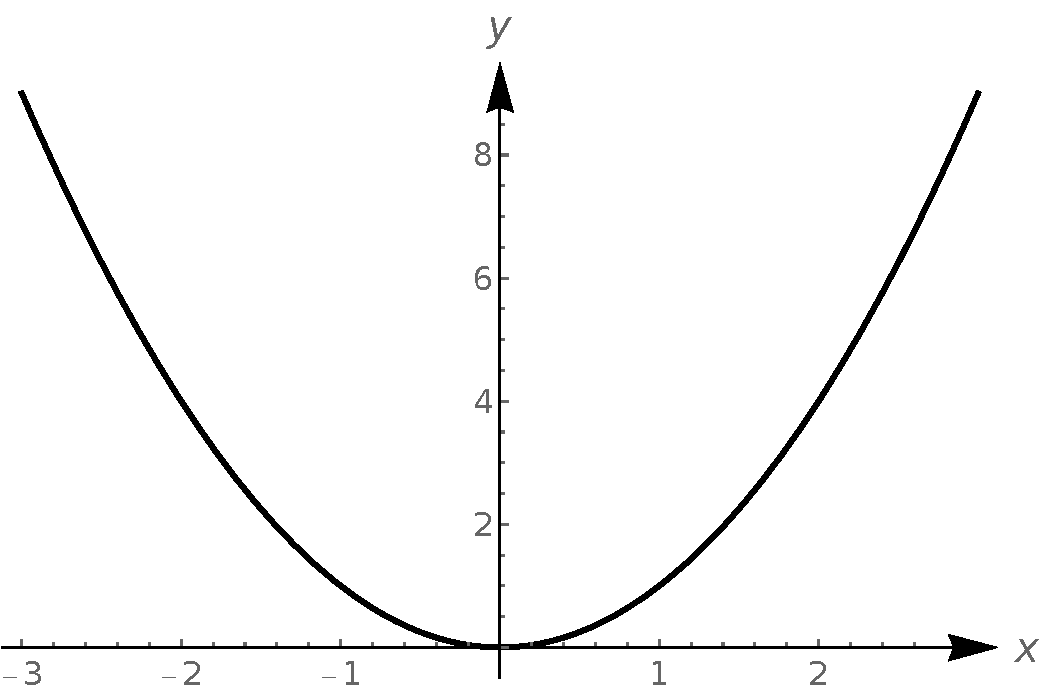
\includegraphics[width=0.3\textwidth]{fig_functions_12a}}
\hspace{1cm}
\subfigure[Graph of $h$ \label{fig_functions_12b}]{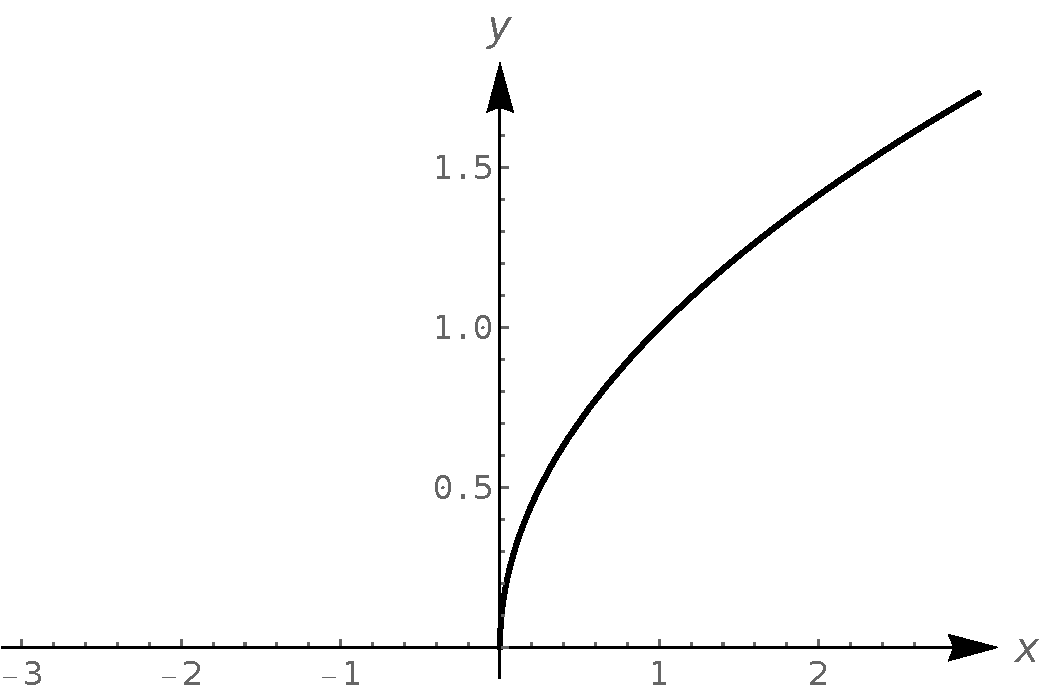
\includegraphics[width=0.3\textwidth]{fig_functions_12b}}
}
\caption{Graphs of the functions $f$, $g$ and $h$ in Example~\ref{example_domain_codomain_range}. }
\label{fig_functions_12}
\end{figure}



\end{example}



\subsection{Function arithmetic}\label{rekenen_functies}
It seems natural that functions should have their own arithmetic which is consistent with the arithmetic of real numbers.  The following definitions allow us to add, subtract, multiply and divide functions using the arithmetic we already know for real numbers.
Suppose $f$ and $g$ are functions and $\dom\,f\cap\dom\,g\neq\emptyset$, then we can define the following operations on $\dom\,f\cap\dom\,g$:
\index{function ! sum}\index[aut]{functie ! som}
\index{function ! difference}\index[aut]{functie ! verschil}
\index{function ! product}\index[aut]{functie ! product}
\index{function ! quotient}\index[aut]{functie ! quoti\"ent}

\begin{itemize}

\item The \textbf{sum} (\textit{som}) of $f$ and $g$: 
 \[(f+g)(x) = f(x) + g(x).\]

\item  The \textbf{difference} (\textit{verschil}) of $f$ and $g$:  
 \[(f-g)(x) = f(x) - g(x).\]

\item  The \textbf{product} (\textit{product}) of $f$ and $g$:
 \[(fg)(x) = f(x)g(x).\]

\item  The \textbf{quotient} (\textit{quoti\"ent}) of $f$ and $g$:
\[\left(\dfrac{f}{g}\right)(x) = \dfrac{f(x)}{g(x)},\] provided $g(x) \neq 0$.

\end{itemize}
  Note that while the formula $(f+g)(x) = f(x) + g(x)$ looks suspiciously like some kind of distributive property, it is nothing of the sort;  the addition on the left hand side of the equation is function addition, and we are using this equation to define the output of the new function $f+g$ as the sum of the real number outputs from $f$ and $g$.

\begin{example}  
 Let $f(x) = 6x^2 - 2x$ and $g(x) = 3-\frac{1}{x}$.  


\begin{enumerate}
\ifvc
\item Find  $(f+g)(-1)$.

\item Find $(fg)(2)$.
\fi


\item  Find the domain of $g-f$. Then find and simplify a formula for  $(g-f)(x)$.

\item  \label{quotdomainex} Find the domain of $g/f$. Then find and simplify a formula for  $\left(\frac{g}{f}\right)(x)$.

\end{enumerate}

\ifanalysis\pagebreak\fi
\ifcalculus\pagebreak\fi
\xhrulefill{gray}{2.5pt}Solution \xhrulefill{gray}{2.5pt}

\begin{enumerate}
\ifvc
\item  To find $(f+g)(-1)$ we first find $f(-1) = 8$ and $g(-1) = 4$. So, we have that $(f+g)(-1) = f(-1) + g(-1) = 8+4 = 12$.

\item To find $(fg)(2)$, we first need $f(2)$ and $g(2)$. Since $f(2) = 20$ and $g(2) = \frac{5}{2}$, our formula yields $(fg)(2) = f(2) g(2) = (20)\left(\frac{5}{2}\right) = 50$.
\fi

\item To find the domain of $g-f$ we need to find the domain of $g$ and of $f$ separately, then find the intersection of these two sets.  Owing to the denominator in the expression $g(x) = 3 - \frac{1}{x}$, we get that the domain of $g$ is $\mathbb{R}_0$.  Since $f(x) = 6x^2-2x$ is valid for all real numbers, we have no further restrictions.  Thus the domain of $g-f$ matches the domain of $g$, namely, $\mathbb{R}_0$.

Moving along, we need to simplify a formula for $(g-f)(x)$.  In this case, we get common denominators and attempt to reduce the resulting fraction.  Doing so, we get

\[ \begin{array}{rclr}
(g-f)(x) & = & g(x) - f(x) & \\ [5pt]
         & = & \left(3-\dfrac{1}{x}\right) - \left(6x^2 - 2x\right) &\\  [10pt]
         & = & \dfrac{-6x^3+2x^2+3x-1}{x}. & \\   
\end{array}\] 

\item  First, we  find the domain of $g$ and $f$ separately, and find the intersection of these two sets.  In addition, since $\left(\frac{g}{f}\right)(x) = \frac{g(x)}{f(x)}$, we are introducing a new denominator, namely $f(x)$, so we need to guard against this being $0$ as well.  The domain of $g$ is $\mathbb{R}_0$ and the domain of $f$ is $\mathbb{R}$.  Setting $f(x) = 0$ gives $6x^2 - 2x = 0$ or $x = 0$ or $x=\frac{1}{3}$.  So, the domain of $g/f$ is $\mathbb{R}\setminus \{0,\tfrac{1}{3}\}$.

Next, we find and simplify a formula for $\left(\frac{g}{f}\right)(x)$.
\renewcommand{\arraystretch}{2.5}
 \allowdisplaybreaks
 \begin{align*}
\left( \dfrac{g}{f}\right)(x) & =  \dfrac{g(x)}{f(x)}\\
    & =  \dfrac{3-\dfrac{1}{x}\vphantom{\left(\dfrac{1}{x}\right)}}{6x^2 - 2x}=\dfrac{3x-1}{\left(6x^2 - 2x\right)x}  \\
	& =  \dfrac{3x-1}{2x^2(3x-1)} \qquad (\text{Assuming }x\neq\frac{1}{3}\; \text{ and } \; x \neq 0) \\
	& =  \dfrac{1}{2x^2}  
\end{align*}
\renewcommand{\arraystretch}{1}
\end{enumerate}
\end{example}

In addition to operations on functions, we can also compose functions. Function composition is defined below.
\begin{definition}[Composite function]
\label{functioncompositiondefn} Suppose $f$ and $g$ are two functions.  The \index{function ! composite}\index[aut]{functie ! samengestelde}\textbf{composite} (\textit{samenstelling}) of $g$ with $f$, denoted $g \circ f$, is defined by
 $$
(g \circ f) (x) = g(f(x))\,,
$$
provided $x\in\dom\,f$  and $f(x)\in\dom\, g$. 
\end{definition}
The quantity $g \circ f$ is also read $g$ composed with $f$ or, more simply $g$ of $f$. At its most basic level, Definition \ref{functioncompositiondefn} tells us to obtain the formula for $\left(g \circ f\right)(x)$, we replace every occurrence of $x$ in the formula for $g(x)$ with the formula we have for $f(x)$.  If we take a step back and look at this from a procedural, inputs and outputs perspective, Defintion \ref{functioncompositiondefn} tells us  the output from $g \circ f$ is found by taking the output from $f$, $f(x)$,  and then making that the input to $g$.  The result, $g(f(x))$, is the output from $g \circ f$. This is illustrated in Figure~\ref{fig_functions_13} for a setting where $f:x\mapsto x^2$ and $g:x\mapsto x+1$. 
\begin{figure}
	\begin{center}
	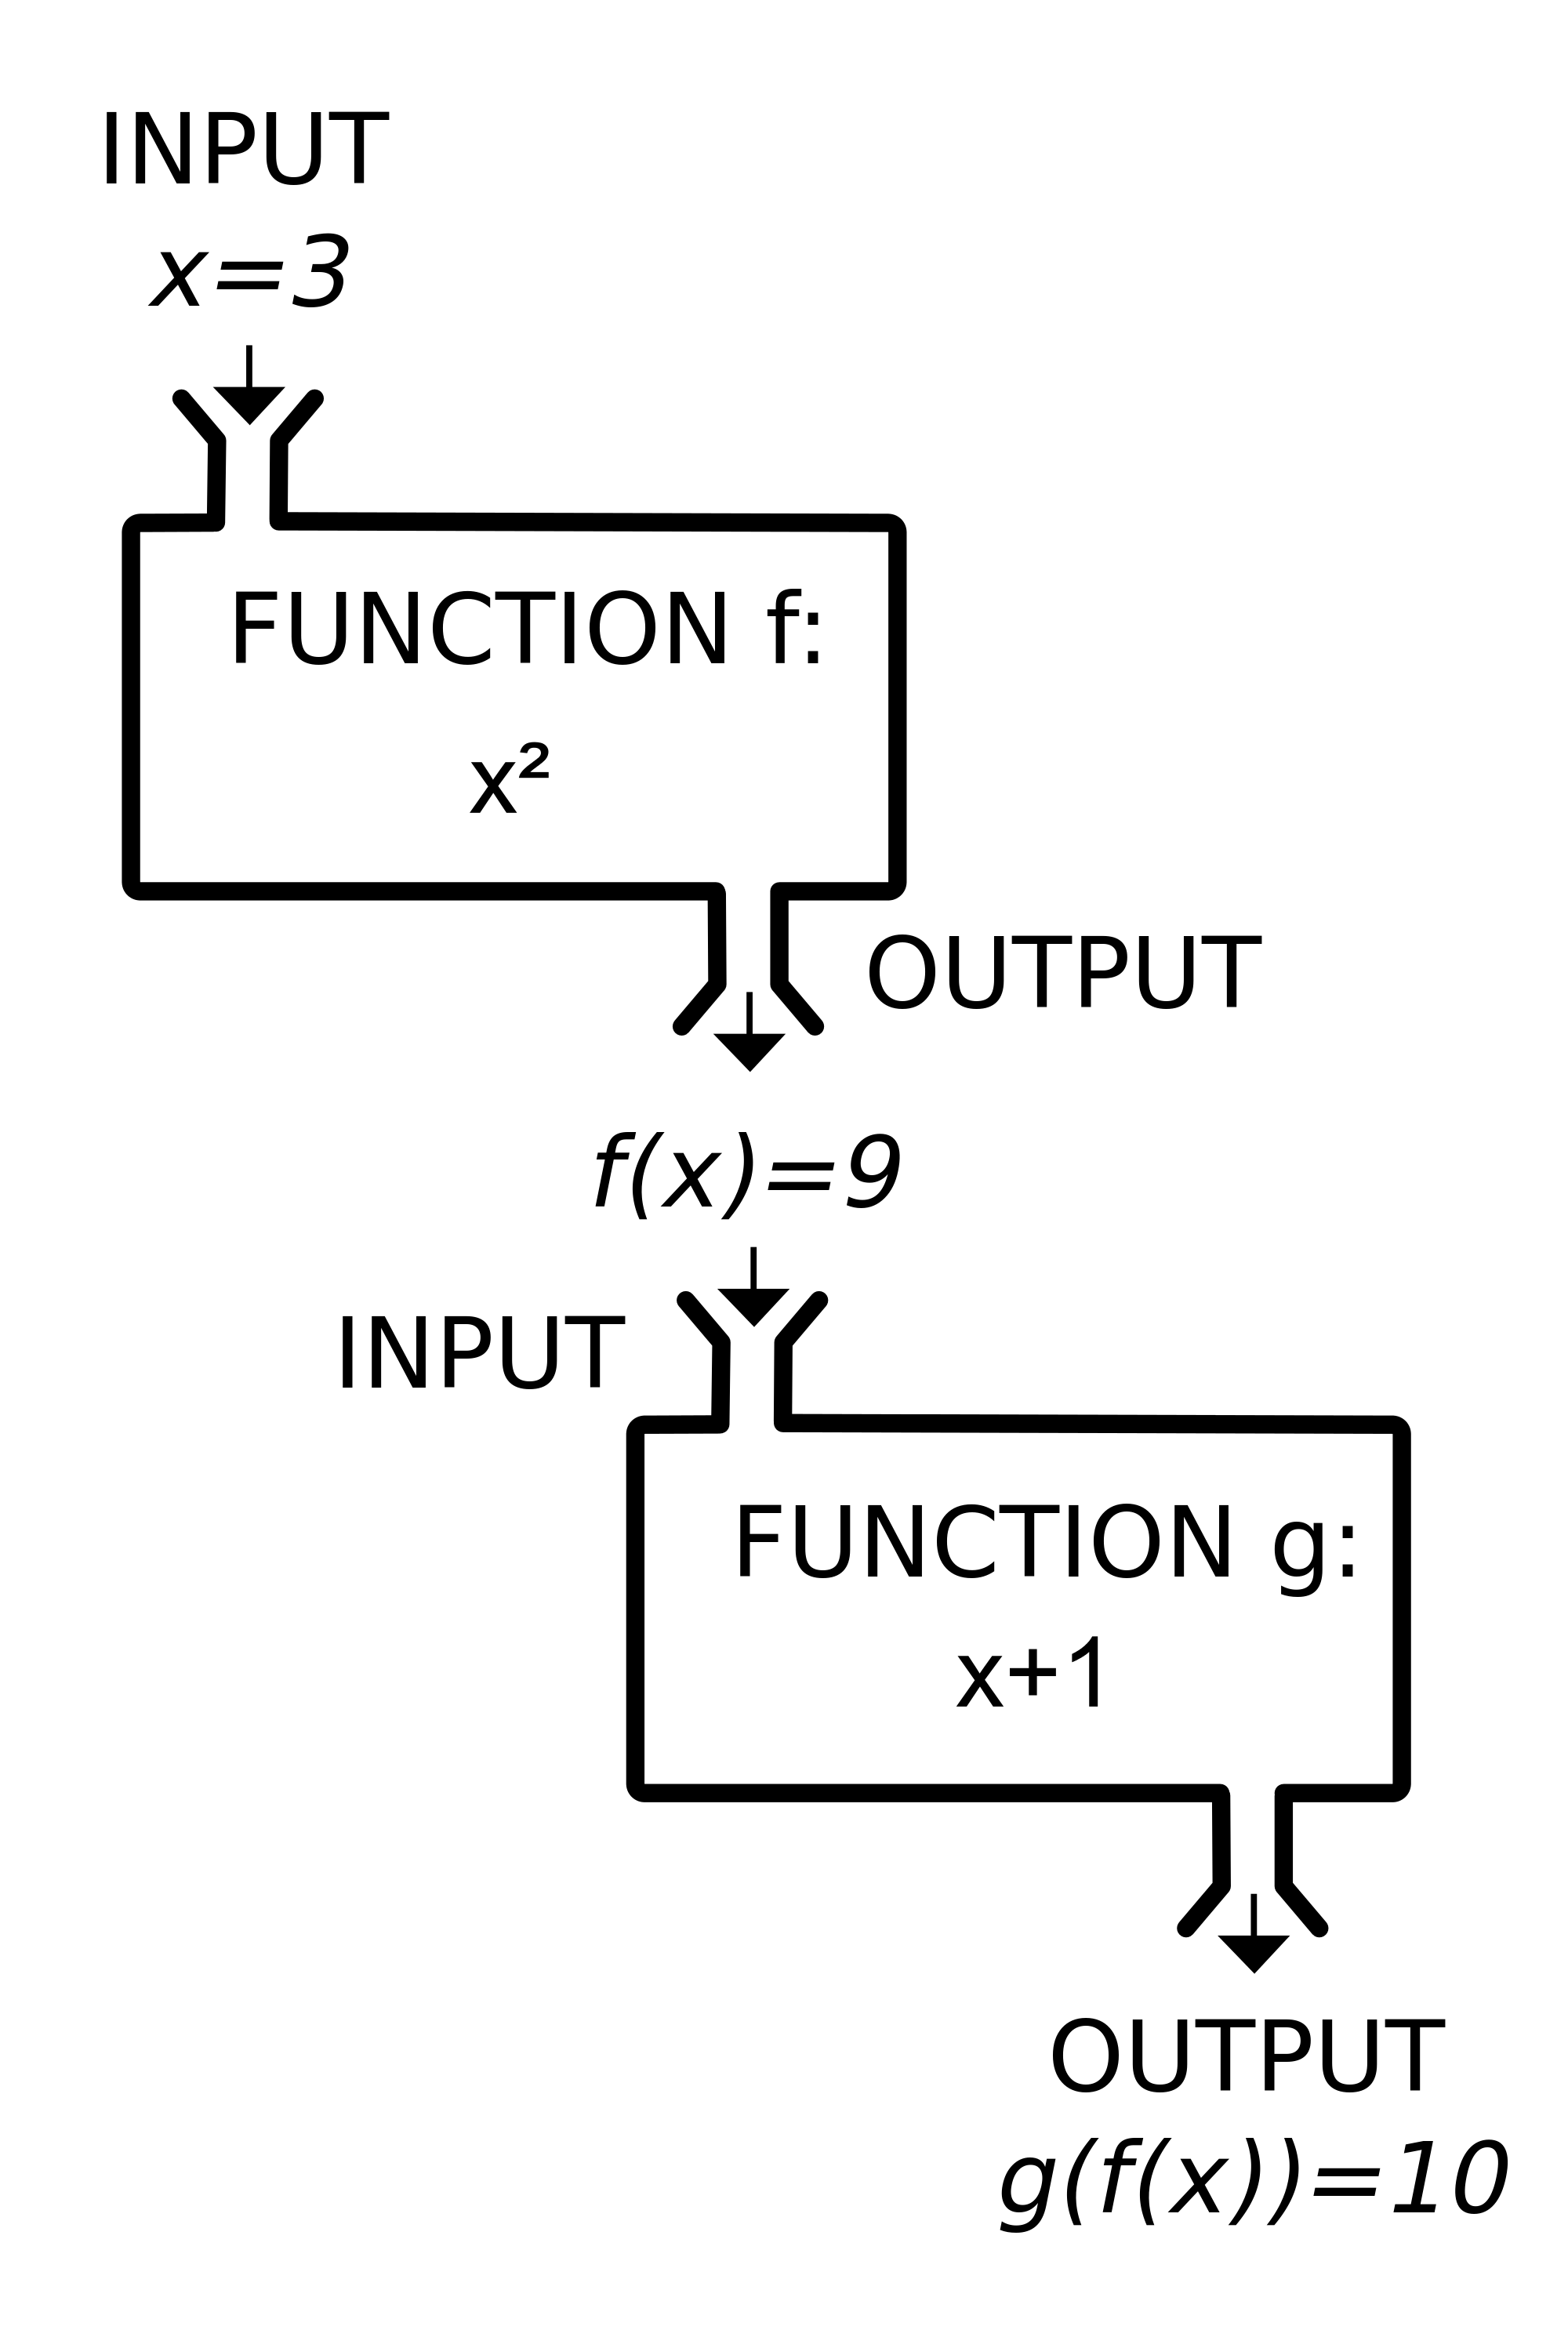
\includegraphics[width=0.3\textwidth]{fig_functions_13}
	\caption{Function composition $(g\circ f)(x)$, where $f:x\mapsto x^2$ and $g:x\mapsto x+1$.}
	\label{fig_functions_13}
	\end{center}
\end{figure}
Clearly, the notion of function composition can easily be generalised to an arbitrary number of functions. For instance,  suppose $f$, $g$ and $h$ are three functions, then we may consider 
$$\left(\left(h \circ g\right) \circ f\right)(x) = h\left(g\left(f\left(x\right)\right)\right).$$




In the expression $g(f(x))$, the function $f$ is often called the inside function while $g$ is often called the outside function.  There are two ways to go about evaluating composite functions - inside out and outside in - depending on which function we replace with its formula first.  Both ways are  demonstrated in the following example.  

\begin{example}
\label{fcexform}
 Let $f(x) = x^2-4x$, \;  $g(x) = 2-\sqrt{x+3}$\; and  $h(x) = \dfrac{2x}{x+1}.$ \\
 \\
 Find and simplify the indicated composite functions. State the domain of each.

\begin{enumerate}
\begin{multicols}{2}
\item  $(g \circ f)(x)$ \label{fcexformfirst}
\item  $\big(h \circ (g \circ f)\big)(x)$ 
\end{multicols}

\end{enumerate}

\xhrulefill{gray}{2.5pt}Solution \xhrulefill{gray}{2.5pt}

\begin{enumerate}
\item  By definition, $(g \circ f)(x) = g(f(x))$. We now illustrate two ways to approach this problem.

\begin{itemize}

\item  Inside out:  We insert the expression $f(x)$ into $g$ first to get  \[(g \circ f)(x) = g(f(x)) = g\left(x^2-4x\right) = 2 - \sqrt{\left(x^2-4x\right)+3} = 2 - \sqrt{x^2-4x+3}.\] 


\item  Outside in:  We use the formula for $g$ first to get  \[(g \circ f)(x) = g(f(x)) = 2 - \sqrt{f(x)+3}  = 2 - \sqrt{\left(x^2-4x\right)+3} = 2 - \sqrt{x^2-4x+3}.\]
 We get the same answer as before.

\end{itemize} 

To find the domain of $g \circ f$, we need to find the elements in the domain of $f$ whose outputs $f(x)$ are in the domain of $g$.  We accomplish this by determining the domain before we simplify the formula for the composite function.  To that end, we examine $(g \circ f)(x) = 2 - \sqrt{\left(x^2-4x\right)+3}$.  To ensure that the argument of the square root is positive, it should hold that $x^2-4x+3 \geq 0$. 
We find the zeros of $x^2-4x+3$ to be $x = 1$ and $x = 3$. Consequently,  the domain of $g \circ f$, is $\left.\right]-\infty, 1] \cup [3,+\infty\left[\right.$. Figure~\ref{fig_functions_14} shows the graph of  $f(x)$, $g(x)$ and  $(g \circ f)$. 
\begin{figure}[H]
\centering
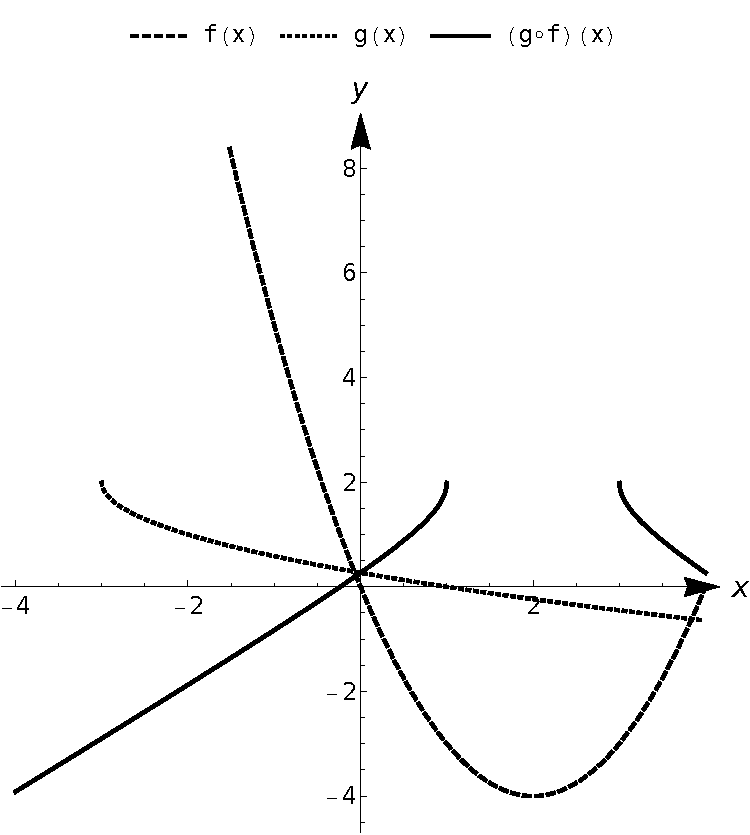
\includegraphics[width=0.45\textwidth]{fig_functions_14}
\caption{Graph of  $f(x)$, $g(x)$ and  $(g \circ f)$ in Example~\ref{fcexform}. \label{fig_functions_14}}
\end{figure}


\item  The expression $\big(h \circ (g \circ f)\big)(x)$ indicates that we first find the composite, $g \circ f$ and compose the function $h$ with the result.  We know already that $(g \circ f)(x) =  2 - \sqrt{x^2-4x+3}$.  We now proceed as usual.

\begin{itemize}

\item  Inside out: We insert the expression $(g \circ f)(x)$ into $h$ first to get

\begin{tabular}{rclr} $\big(h \circ (g \circ f)\big)(x)$ & = & $h\big((g \circ f)(x)\big)=h\left(2 - \sqrt{x^2-4x+3}\right)$  & \\ [0.8cm]
 & = & $\dfrac{2 \left(2 - \sqrt{x^2-4x+3}\right)}{\left(2 - \sqrt{x^2-4x+3}\right)+1}=\dfrac{4 - 2\sqrt{x^2-4x+3}}{3 - \sqrt{x^2-4x+3}}$. & \\ 
 %& = & $\dfrac{4 - 2\sqrt{x^2-4x+3}}{3 - \sqrt{x^2-4x+3}}$. & \\
 \end{tabular}

\item  Outside in:  We use the formula for $h(x)$ first to get

\begin{tabular}{rclr} $\big(h \circ (g \circ f)\big)(x)$ & = & $h\big((g \circ f)(x)\big)=\dfrac{2 \left( (g \circ f)(x)\right)}{  \left( (g \circ f)(x)\right) + 1}$  & \\ [0.8cm]
& = & $\dfrac{2 \left(2 - \sqrt{x^2-4x+3}\right)}{\left(2 - \sqrt{x^2-4x+3}\right)+1}=\dfrac{4 - 2\sqrt{x^2-4x+3}}{3 - \sqrt{x^2-4x+3}}$. & \\ 
 \end{tabular}
 
 \end{itemize}
 
To find the domain of $(h \circ (g \circ f))$, we look at the step before we began to simplify, 
\[(h \circ (g \circ f))(x) = \frac{2 \left(2 - \sqrt{x^2-4x+3}\right)}{\left(2 - \sqrt{x^2-4x+3}\right)+1}.\] 
 For the square root, we need $x^2-4x+3 \geq 0$, which requires $\left.\right]-\infty, 1] \cup [3,+\infty\left[\right.$.  Next, we set the denominator to zero and solve:  $\left(2 - \sqrt{x^2-4x+3}\right)+1 = 0$.  We get $\sqrt{x^2-4x+3} = 3$, and, after squaring both sides, we have $x^2-4x+3 = 9$.  To solve $x^2-4x-6 = 0$, we use the quadratic formula and get $x = 2 \pm \sqrt{10}$.   Hence we must exclude these numbers from the domain of $h \circ (g \circ f)$.  Consequently our final domain for $h \circ (f \circ g)$ is $$\left]\,-\infty, 2 -\sqrt{10}\,\right[ \cup \left]\, 2 - \sqrt{10}, 1\,\right] \cup \left[\, 3, 2 + \sqrt{10}\, \right[ \cup \left]\,2+\sqrt{10}, \infty\,\right[\,.$$

.

\end{enumerate}
\end{example}




From this example, we learn that  function composition is not commutative, so $\left(g \circ f\right)(x)\neq \left(f \circ g\right)(x)$, though it is associative, i.e.\ it holds that
\index{commutativity}\index[aut]{commutativiteit}\index{associativity}\index[aut]{associativiteit}
$$
\left(\left(h \circ g\right) \circ f\right)(x)=\left(h \circ \left(g \circ f\right)\right)(x)\,.
$$
Also note the importance of finding the domain of the composite function before simplifying.


\ifvc

In practice, function composition is often used to relate two quantities which may not be directly related, but have a variable in common, as illustrated in our next example.

\begin{example}
  The surface area $S$ [L$^2$] of a sphere is a function of its radius $r$ [L] and is given by the formula $S(r) = 4 \pi r^2$.  Suppose the sphere is being inflated so that the radius of the sphere is increasing according to the formula $r(t) = 3t^2$, where $t$ [T] is measured in seconds, $t \geq 0$, and $r$ is measured in centimetres.  Find and interpret $(S \circ r)(t)$.

\xhrulefill{gray}{2.5pt}Solution \xhrulefill{gray}{2.5pt}

 Given a specific time, $t$, we could find the radius at that time, $r(t)$ and feed that into $S(r)$ to find the surface area at that time.  From this we see that the surface area $S$ is ultimately a function of time $t$ and we find 
$$(S \circ r)(t) = S(r(t)) = 4 \pi (r(t))^2 = 4 \pi \left(3t^2\right)^2 = 36 \pi t^{4}.$$  
This formula allows us to compute the surface area directly given the time. 

\end{example}

A useful skill in calculus is to be able to take a complicated function and break it down into a composition of easier functions which our last example illustrates.

\begin{example}
Write  the  function
$$
G(x) = \dfrac{2}{x^2+1}
$$
 as a composition of two or more functions.  Check your answer by performing the function composition.

\xhrulefill{gray}{2.5pt}Solution \xhrulefill{gray}{2.5pt}

We attack decomposing $G$ from an operational approach.  Given an input $x$, the first step is to square $x$, then add $1$, then divide $2$ by the result.  We will assign each of these steps a function so as to write $G$ as a composite of three functions: $f$, $g$ and $h$.  Our first function, $f$, is the function that squares its input, $f(x) = x^2$.  The next function is the function that adds $1$ to its input, $g(x) = x+1$.  Our last function takes its input and divides it into $2$, $h(x) = \frac{2}{x}$.  The claim is that $G = h \circ g \circ f$. We find  
\[(h \circ g \circ f)(x) = h(g(f(x))) = h(g\left(x^2\right)) = h\left(x^2+1\right)= \frac{2}{x^2+1} = G(x),\]
 so we are done.

\end{example}

\fi



\subsection{Function properties}\label{eig_functies}
When graphing functions, we will typically investigate whether or not there is some kind of symmetry to its graph, whether or not it is periodic, and so on. 

\subsubsection{Injections, surjections and bijections}
Injections, surjections and bijections are classes of functions distinguished by the manner in which arguments  and images are mapped to each other. 

\begin{definition}[Injective, surjective and bijective]\label{injsurjbij}
A function $ f:\;X\to Y$ is called 
\vspace{-0.3cm}
\begin{itemize}
\item \textbf{injective} (\textit{injectief}) (one-to-one) if each element of the codomain is mapped to by at most one element of the domain. Mathematically, we may write:
$$
\forall\,x_1,\,x_2\in\dom\,f:\,f(x_1)=f(x_2)\Rightarrow\,x_1=x_2\,.
$$
This implies that two different elements belonging to the function's domain cannot be mapped to the same element in its codomain, so every straight line parallel to the $x$-axis intersects the graph of $f$ in at most one point. An injective function is an \textbf{injection} (\textit{injectie});
\item \textbf{surjective} (\textit{surjectief}) (onto) if each element of the codomain is mapped to by at least one element of the domain. That is, the range and the codomain of the function are equal. This implies that every straight line parallel to the $x$-axis intersects the graph of $f$ in at least one point. A surjective function is a \textbf{surjection} (\textit{surjectie}); and
\item \textbf{bijective} (\textit{bijectief}) (one-to-one correspondence) if each element of the codomain is mapped to by exactly one element of the domain. So, the function is both injective and surjective. This implies that every straight line parallel to the $x$-axis intersects the graph of $f$ in at exactly one point. A bijective function is a \textbf{bijection} (\textit{bijectie}).
\end{itemize}
\end{definition}
The four possible combinations of injective and surjective features are illustrated in Table~\ref{tab_functions_1}.
An injective function does not need to be surjective  because not all elements of the codomain may be associated with arguments, and likewise a surjective function does not need to be injective as some images may be associated with more than one argument. \index{injection}\index[aut]{injectie}
\index{function ! injective}\index[aut]{functie ! injectief}
\index{surjection}\index[aut]{surjectie}
\index{function ! surjective}\index[aut]{functie ! surjectief}
\index{bijection}\index[aut]{bijectie}
\index{function ! bijective}\index[aut]{functie ! bijectief}

\begin{table}
\caption{The four possible combinations of injective and surjective features.}
	\label{tab_functions_1}
\begin{center}
	\begin{tabular}{m{0.15\textwidth} >{\centering\arraybackslash}m{0.25\textwidth} >{\centering\arraybackslash}m{0.25\textwidth}}
	&Surjective&Non-surjective\\
	Injective&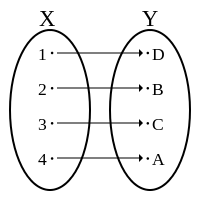
\includegraphics[width=0.225\textwidth]{fig_functions_15a}&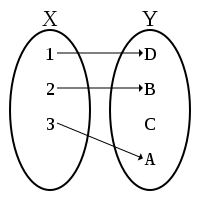
\includegraphics[width=0.225\textwidth]{fig_functions_15b}\\
	Non-injective&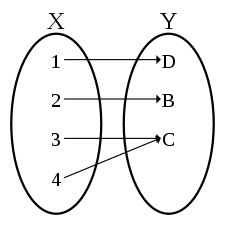
\includegraphics[width=0.225\textwidth]{fig_functions_15c}&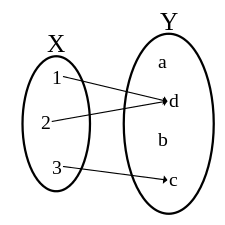
\includegraphics[width=0.225\textwidth]{fig_functions_15d}\\
	\end{tabular}
\end{center}
\end{table}

\begin{example}
\label{exinjectief}
Determine whether the following real functions are injections, surjections and/or bijections.
\begin{multicols}{3}
\begin{enumerate}
\item $f:\mathbb{R}^+\to\mathbb{R}:\,x\mapsto \sqrt{x}$
\item $g:\mathbb{R}\to\mathbb{R}:\,x\mapsto x^2$
\item $h:\mathbb{R}\to\mathbb{R}:\,x\mapsto x^3$
\end{enumerate}
\end{multicols}
\vfill



\xhrulefill{gray}{2.5pt}Solution \xhrulefill{gray}{2.5pt}
\ifmathematica
Figure~\ref{fig_functions_16} depicts the graphs of the considered functions, which were generated in Mathematica.
\fi
\ifpython
Figure~\ref{fig_functions_16} depicts the graphs of the considered functions, which were generated in Python.
\fi
\begin{enumerate}
\item For any two elements $x_1$ and $x_2$ of this function's domain, it holds that if $\sqrt{x_1}=\sqrt{x_2}$, then $x_1=x_2$. This means that every straight line parallel to the $x$-axis intersects with the function's graph in at most one point (Figure~\ref{fig_functions_16a}), so the function $f$ is an injection. Since the range of this function is restricted to $\mathbb{R}^+$, whereas its codomain is $\mathbb{R}$, this function is non-surjective, and hence it cannot be a bijection. 
\item Since we have for any two elements $x_1$ and $x_2$ of this function's domain that if $x_1^2=x_2^2$ then $x_1=\pm x_2$, this function is non-injective. Besides, it is neither a surjection because its range is $\mathbb{R}^+$, whereas its codomain is $\mathbb{R}$. Consequently, it is not a bijection (Figure~\ref{fig_functions_16b}). 
\item For any two elements $x_1$ and $x_2$ of this function's domain, it holds that if $x_1^3=x_2^3$, then $x_1=x_2$. So the function $h$ is an injection. Moreover, it is also a surjection because its range is $\mathbb{R}$; that is every straight line parallel to the $x$-axis intersects with the function's graph in at least one point. Since  $h$ is both an injection and surjection, it is a bijection (Figure~\ref{fig_functions_16c}).
\end{enumerate}


\begin{figure}[H]
\centering
%\raisebox{0.5cm}{
\centerline{
\subfigure[Graph of $f$ \label{fig_functions_16a}]{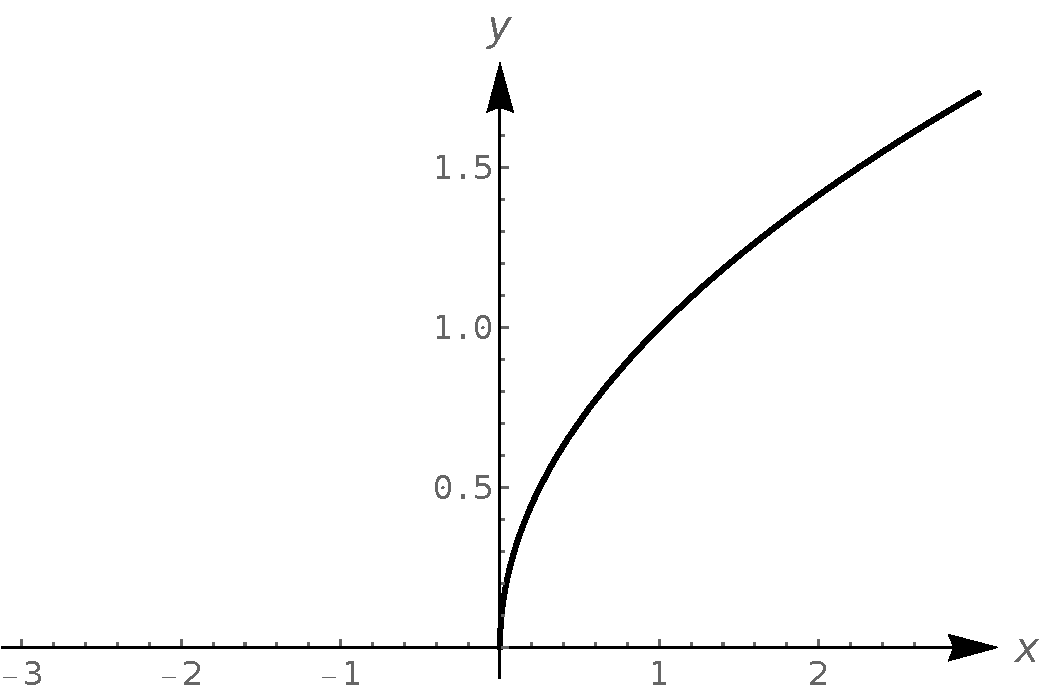
\includegraphics[width=0.3\textwidth]{fig_functions_12b}}
\hspace{0.1cm}
\subfigure[Graph of $g$ \label{fig_functions_16b}]{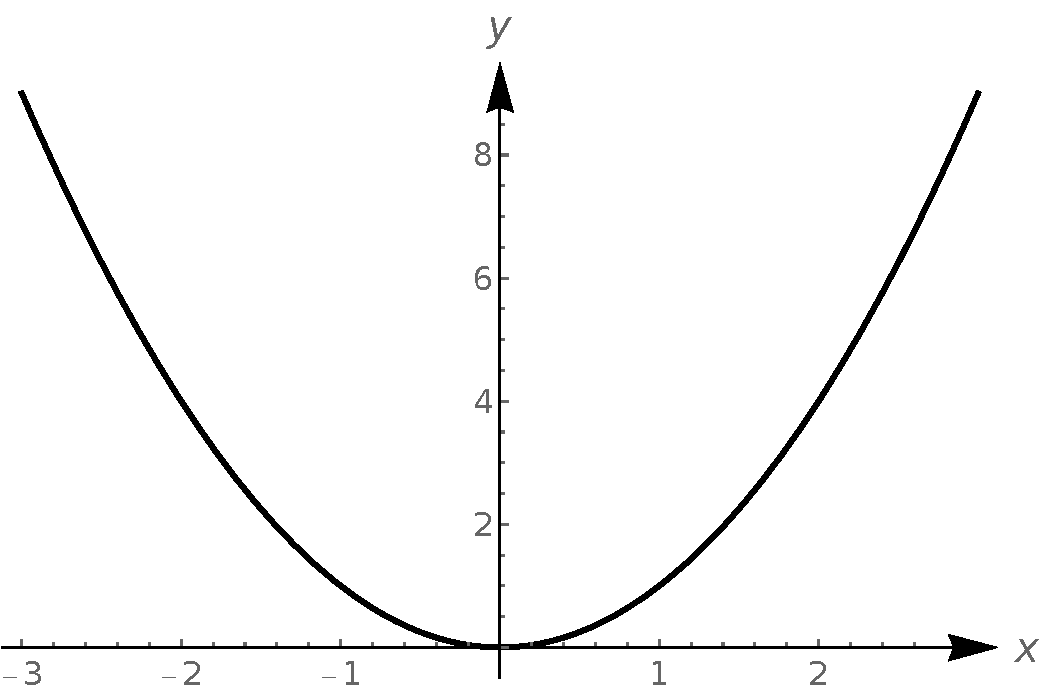
\includegraphics[width=0.3\textwidth]{fig_functions_12a}}
\hspace{0.1cm}
\subfigure[Graph of $h$ \label{fig_functions_16c}]{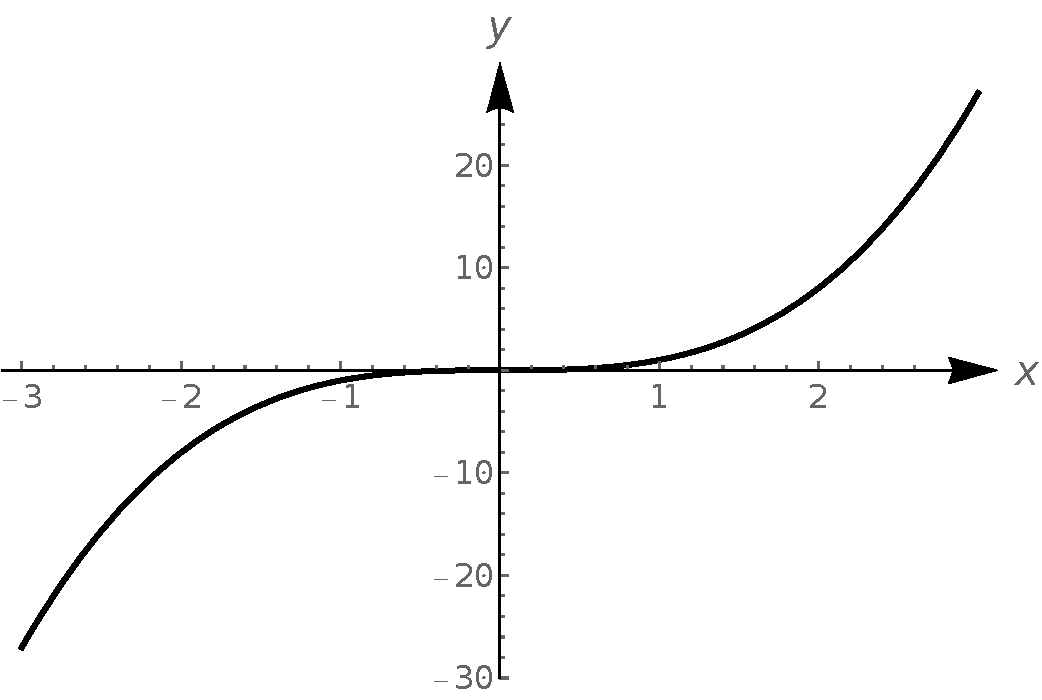
\includegraphics[width=0.3\textwidth]{fig_functions_16c}}
}
\caption{Graphs of the functions $f$, $g$ and $h$ in Example~\ref{exinjectief}. }
\label{fig_functions_16}
\end{figure}



\end{example}


\subsubsection{Symmetry}
Of the three symmetries discussed in Section \ref{relaties}, only two are of significance to functions:  symmetry about the $y$-axis and symmetry about the origin. 
%Hence,  we need $f(-x) = f(x)$ for all $x$ in the function's domain, to guarantee that the graph of the function $f$ is symmetric about the $y$-axis to have a so-called $\textbf{even}$ (\textit{even}) function. \index{function ! even}\index{even function} \index[aut]{functie ! even}\index[aut]{even functie} In a similar fashion, we need $-f(-x) = f(x)$, or, equivalently, $f(-x) = -f(x)$ for all $x$ in the function's domain to have an \textbf{odd} (\textit{oneven}) function $f$. \index{function ! odd}\index{odd function} \index[aut]{functie ! oneven}\index[aut]{oneven functie}



\begin{definition}[Even/odd functions]\label{evenoddfun}
A function $f$ is
\vspace{-0.3cm}
\begin{itemize}
\item an $\textbf{even}$ (\textit{even}) function\index{function ! even}\index{even function}\index[aut]{functie ! even}\index[aut]{even functie} if and only if $f(-x) = f(x)$ for all $x\in\dom\,f$. The graph of $f$ is symmetric about the $y$-axis.
\item an \textbf{odd} (\textit{oneven}) function\index{function ! odd}\index{odd function}\index[aut]{functie ! oneven}\index[aut]{oneven functie} if and only if $-f(-x) = f(x)$, or, equivalently, $f(-x) = -f(x)$ for all $x\in\dom\,f$. The graph of $f$ is symmetric about the origin.
\end{itemize}
\end{definition}

\begin{example}
\ifmathematica
Determine analytically if the following functions are even, odd, or neither even nor odd.  \ifcourse Verify your result with Mathematica. \fi\fi

\ifpython
Determine analytically if the following functions are even, odd, or neither even nor odd.  \ifcourse Verify your result with Python. \fi\fi

\begin{enumerate}
\begin{multicols}{2}
\item  $f(x) = \dfrac{5}{2 - x^2}$ 
\item  $g(x) = \dfrac{5x}{2 - x^2}$  
\end{multicols}
\end{enumerate}


\xhrulefill{gray}{2.5pt}Solution \xhrulefill{gray}{2.5pt}

\begin{enumerate}
\item The first step  is to replace $x$ with $-x$ and simplify.
$$
f(-x)  =  \dfrac{5}{2 - (-x)^2}=\dfrac{5}{2 - x^2}=f(x) 
$$

Hence, $f$ is even. \ifmathematica\ifcourse This conclusion can be verified in Mathematica using the function \lstinline{Plot}.
\begin{mdframed}[default,backgroundcolor=gray!40,roundcorner=8pt]
\begin{mmaCell}[morefunctionlocal={x}, moredefined={Arrowheads}]{Input}
  Plot[\mmaFrac{5}{2-\mmaSup{x}{2}},\{x,-3,3\},AxesLabel\(\pmb{\to}\)\{"x","y"\},AxesStyle\(\pmb{\to}\)Arrowheads[\{0,0.05`\}]]

\end{mmaCell}


\begin{mmaCell}[moregraphics={moreig={scale=.4}}]{Output}
	 \mmaGraphics{fig_functions_17}
\end{mmaCell}
Here, the option \lstinline{AxesLabel} was used to label the axes, while using the option \lstinline{Arrowheads} we add arrowheads to these axes. 
\end{mdframed}
\fi
\fi

\ifpython\ifcourse This conclusion can be verified in Python using the function \lstinline{plot}.

Here, the option \lstinline{xlabel} and \lstinline{ylabel} were used to label the axes. 
\begin{pyin}
from sympy import symbols
from sympy.plotting import plot
x = symbols('x')
plot(5/(2-x**2), xlim=(-3, 3), ylim=(-15, 15), xlabel="x", ylabel="y", adaptive=False, nb_of_points=1000)
\end{pyin}
\begin{pyout}
|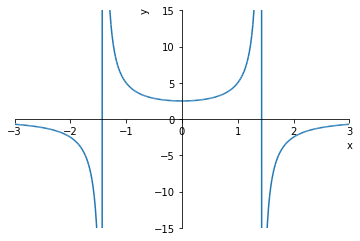
\includegraphics[width=0.5\textwidth]{fig_functions_17_Python}|
\end{pyout}
\fi
\fi

\item Again, we  replace $x$ with $-x$ and simplify.
$$
g(-x)  =  \dfrac{5(-x)}{2 - (-x)^2}  =  \dfrac{-5x}{2 - x^2} =-g(x) 
$$

Clearly, $g$ is odd. \ifvc This is confirmed by the graph of this function.  \fi \ifmathematica\ifcourse This is confirmed by the graph of this function generated in Mathematica: \fi
	\begin{center}
			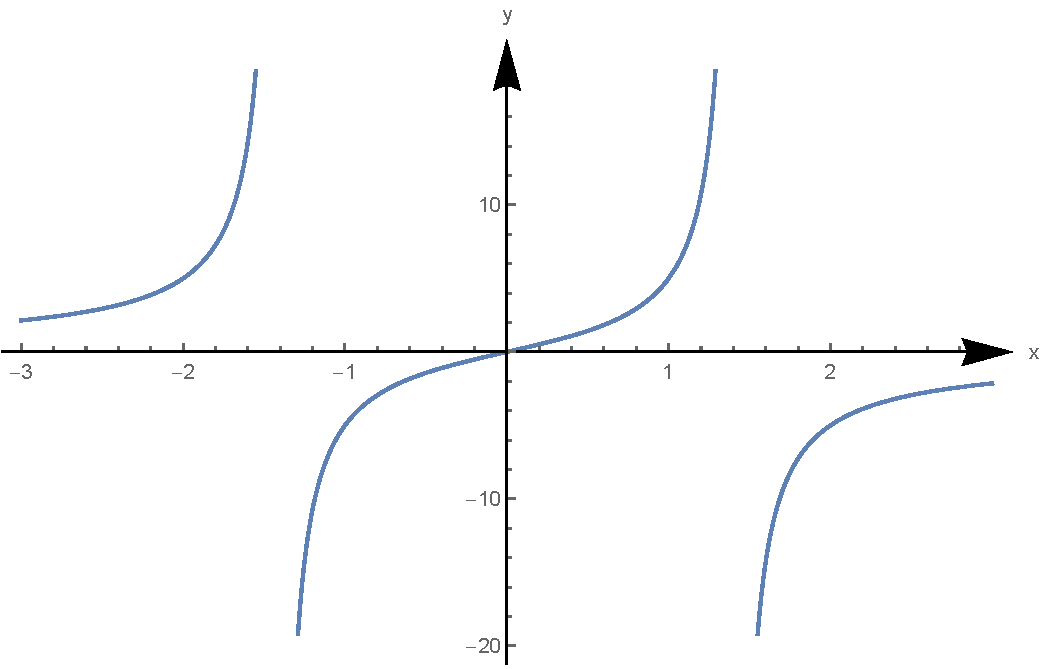
\includegraphics[width=0.4\textwidth]{fig_functions_18}
	\end{center}
\fi

\ifcourse\ifpython This is confirmed by the graph of this function generated in Python: \fi
	\begin{center}
			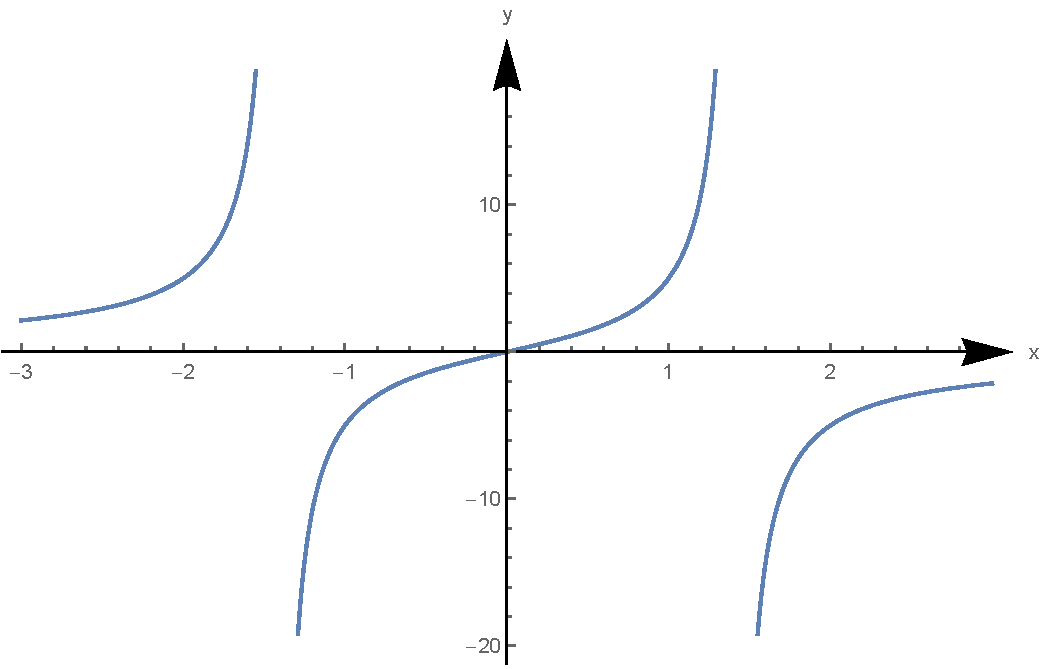
\includegraphics[width=0.4\textwidth]{fig_functions_18}
	\end{center}
\fi

\end{enumerate}
\end{example}



\subsubsection{Periodicity}
\begin{definition}[Periodic function]\label{periodicfunction}
A function $f$ is said to be \textbf{periodic} (\textit{periodiek}) with \textbf{period} (\textit{periode}) $P$ ($P\in\mathbb{R}^+_0$), if 
$$
f(x+P)=f(x)\,,
$$
for all $x\in\dom\,f$. If there exists a least positive constant $P$ with this property, it is called the \textbf{fundamental period}. 
\end{definition}
A function with period $P$ will repeat on intervals of length $P$, and these intervals are referred to as \textbf{periods}.
\index{periodic function}\index[aut]{periodieke functie}
\index{fundamental period}
\index{function ! periodic}\index[aut]{functie ! periodiek}


\subsubsection{Function behaviour}
As you shall see in Chapters~\ref{chap_algebraic} and \ref{chap_trans}, each family of functions has its own unique attributes and we will study them all in great detail.  The purpose of this section is to lay the foundation for that further study by investigating aspects of function behaviour which apply to all functions.  To start, we will examine the concepts of {\bf increasing} (\textit{stijgend}), {\bf decreasing} (\textit{dalend}) and {\bf constant} (\textit{constant}).  Before defining the concepts algebraically, it is instructive to first look at them graphically. For that purpose, consider the graph of a function $f$ in Figure~\ref{fig_functions_19}. 
\index{function ! increasing}\index[aut]{functie ! stijgend}
\index{function ! decreasing}\index[aut]{functie ! dalend}
\index{function ! constant}\index[aut]{functie ! constant}
\index{injection}\index[aut]{injectie}
\index{function ! injective}\index[aut]{functie ! injectief}
\begin{figure}[h]
	\begin{center}
			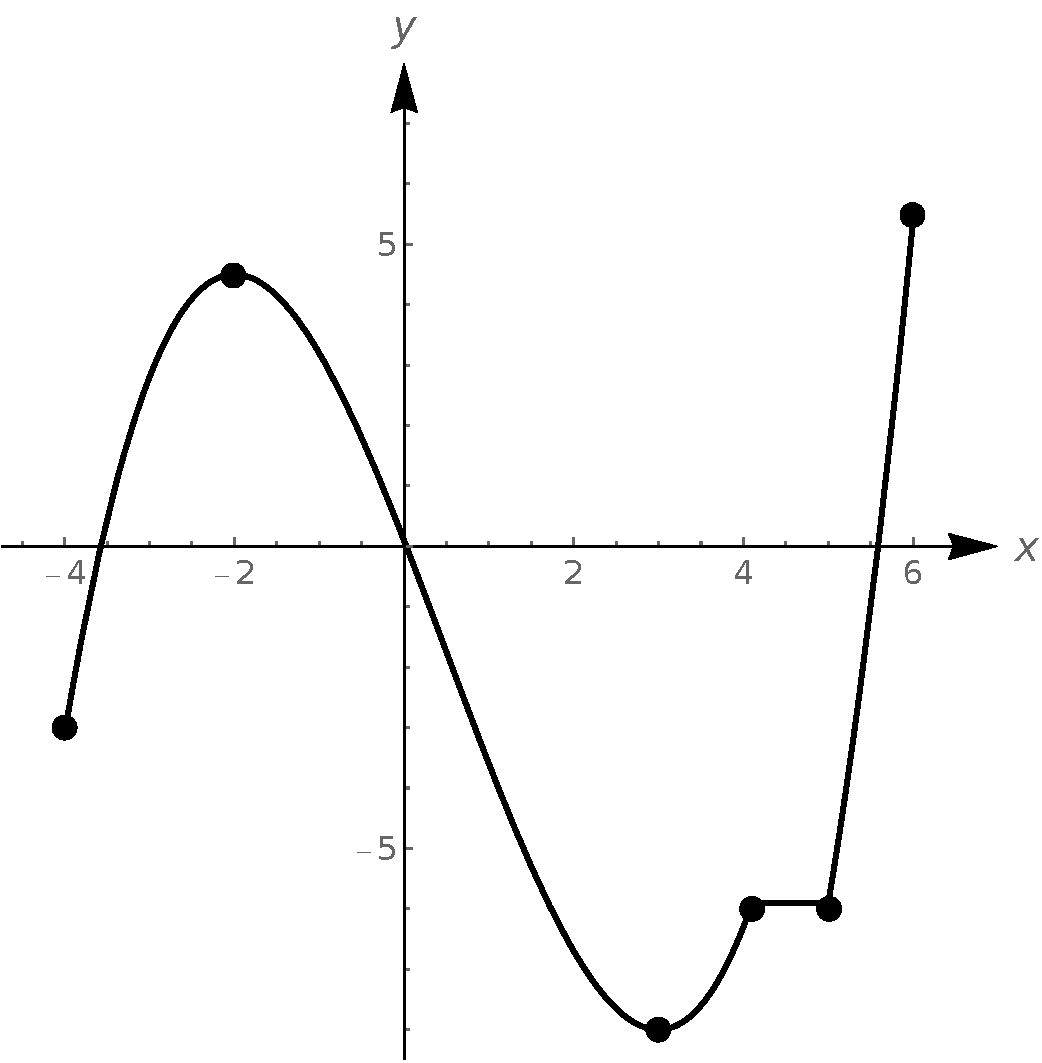
\includegraphics[width=0.45\textwidth]{fig_functions_19}
	\caption{The graph of $y=f(x)$.}
	\label{fig_functions_19}
	\end{center}
\end{figure}


For the $x$ values between $-4$ and $-2$ (inclusive), the $y$-coordinates on the graph are increasing, as we move from left to right.  Hence the function $f$ is increasing on the interval $[-4,-2]$.  Analogously, we say that $f$ is decreasing on the interval $[-2,3]$, increasing once more on the interval $[3,4]$, constant on $[4,5]$, and finally increasing once again on $[5,6]$.  

Let us now introduce more formal algebraic definitions of what it means for a function to be increasing, decreasing or constant.

\ifcalculus
\begin{definition}[Function behaviour]

\label{incdeccnstdefn}

Suppose $f$ is a function defined on an interval $I\subset\dom\,f$.  We say $f$ is:

\vspace{-0.3cm}
\begin{itemize}
\item \textbf{increasing} on $I$ if and only if $f(x_1) \leq f(x_2)$ for all $x_1$, $x_2$ in $I$ with $x_1 < x_2$.

\item \textbf{decreasing} on $I$ if and only if $f(x_1) \geq f(x_2)$ for all  $x_1$, $x_2$ in $I$ with $x_1 < x_2$.

\item \textbf{constant} on $I$ if and only if $f(x_1) = f(x_2)$ for all  $x_1$, $x_2$ in $I$.

\end{itemize}
\end{definition}
\fi

\ifanalysis
\begin{definition}[Function behaviour]

\label{incdeccnstdefn}

Suppose $f$ is a function defined on an interval $I\subset\dom\,f$.  We say $f$ is:
\vspace{-0.3cm}
\begin{itemize}
\item \textbf{increasing} on $I$ if and only if 
$
\forall x_1,x_2\in\,I\mid x_1<x_2\Rightarrow f(x_1) \leq f(x_2)\,.
$

\item \textbf{decreasing} on $I$ if and only if 
$
\forall x_1,x_2\in\,I\mid x_1<x_2\Rightarrow f(x_1) \geq f(x_2)\,.
$

\item \textbf{constant} on $I$ if and only if
$
\forall x_1,x_2\in\,I\mid x_1<x_2\Rightarrow f(x_1) =f(x_2)\,.
$

\end{itemize}
\end{definition}
\fi

If the order $\leq$ in the definition of an increasing function is replaced by $<$,  we say that $f$ is \textbf{strictly increasing} (\textit{strikt stijgend}) on the interval $I$, and likewise for a \textbf{strictly decreasing} (\textit{strikt dalend}) function. Clearly, if $f$ is either strictly increasing or decreasing on an interval $I$, it must hold that $f$ is an injective function .  
\index{function ! strictly increasing}\index[aut]{functie ! strikt stijgend}
\index{function ! strictly decreasing}\index[aut]{functie ! strikt dalend}

We say that functions are \textbf{monotonically} (\textit{monotoon}) increasing or decreasing on the interval $I$ if they are entirely non-decreasing or entirely non-increasing, respectively. For instance, a function that increases monotonically does not exclusively have to increase, it simply must not decrease (Figure~\ref{fig_functions_20a}). On the other hand, a function is \textbf{strictly monotone} (\textit{strikt monotoon}) on the interval $I$ if it is either strictly increasing or decreasing on that interval. 
\index{function ! monotone} \index[aut]{functie ! monotoon}
\index{function ! strictly increasing}\index[aut]{functie ! strikt stijgend}
\index{function ! strictly decreasing}\index[aut]{functie ! strikt dalend}
\index{function ! strictly monotone} \index[aut]{functie ! strikt monotoon}
\begin{figure}
\centering
%\raisebox{0.5cm}{
\centerline{
\subfigure[\label{fig_functions_20a}]{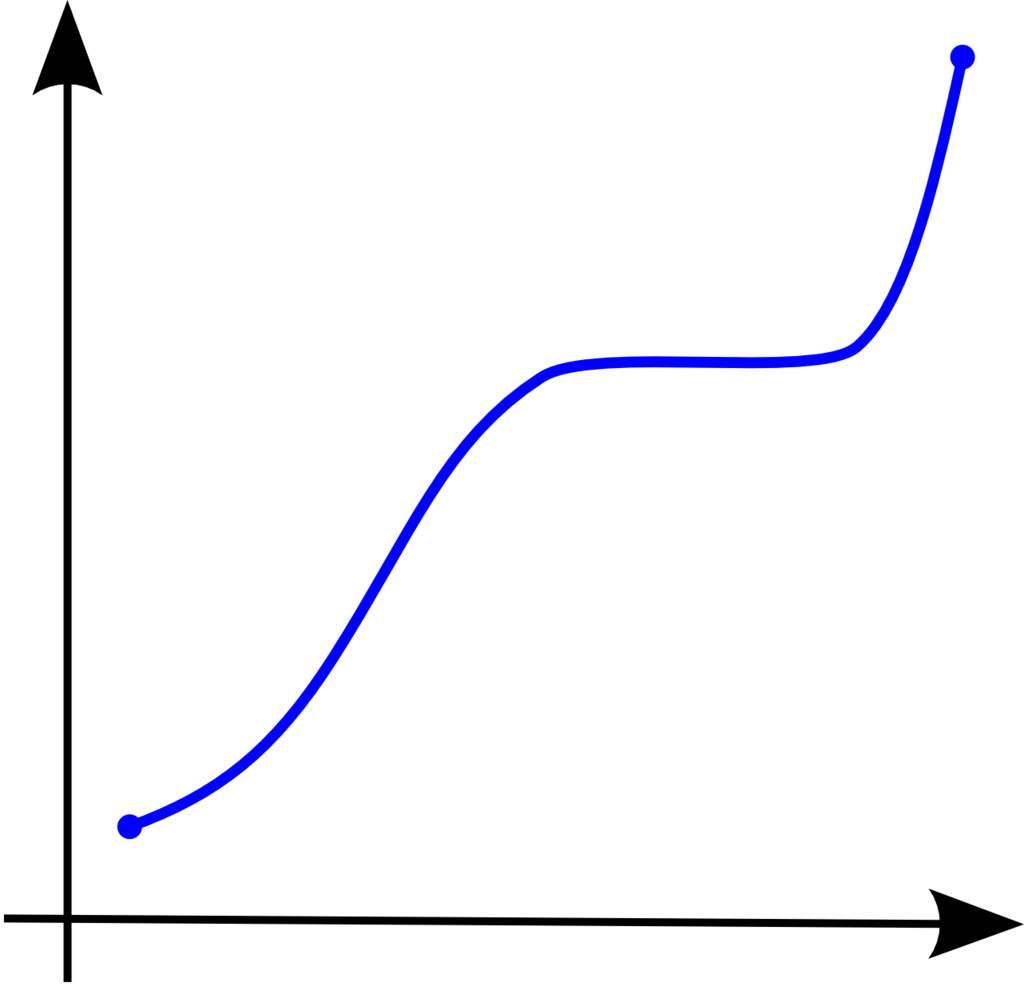
\includegraphics[width=0.25\textwidth]{fig_functions_20a}}
\hspace{0.5cm}
\subfigure[ \label{fig_functions_20b}]{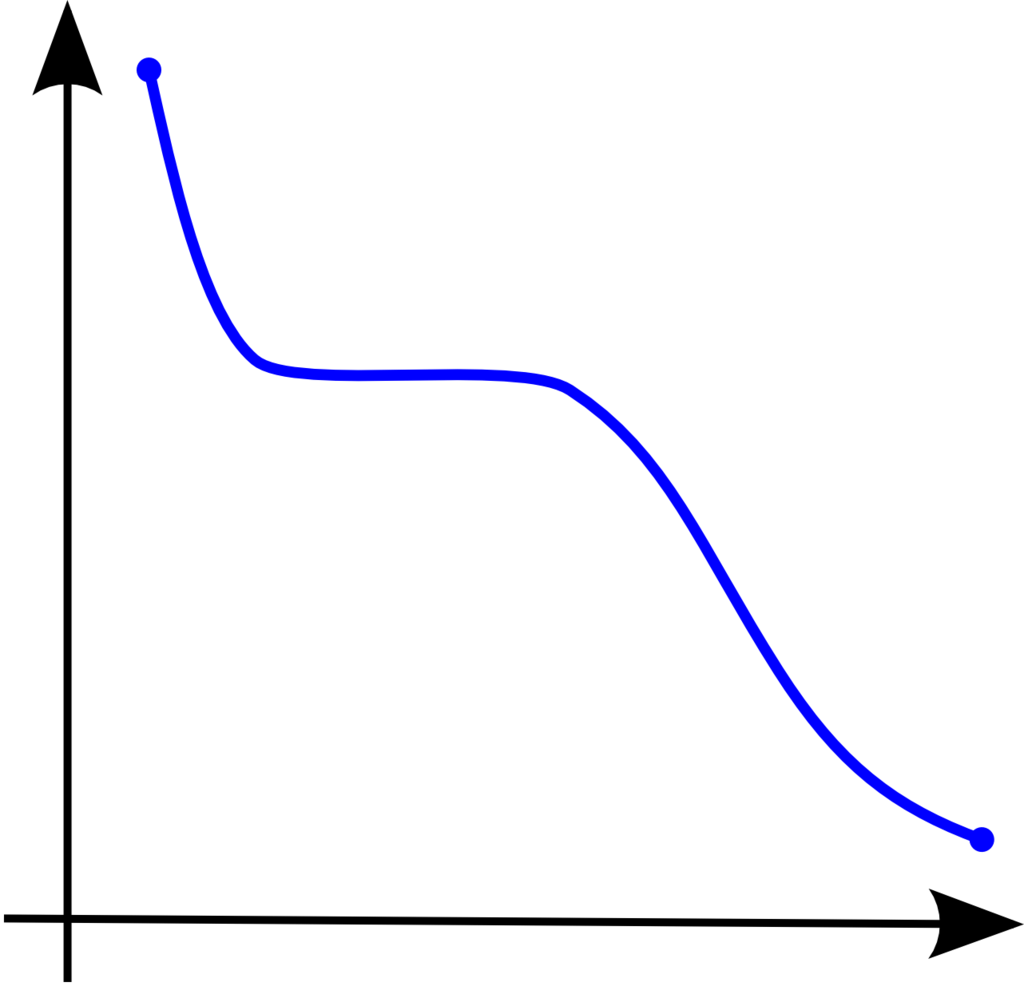
\includegraphics[width=0.25\textwidth]{fig_functions_20b}}
}
\caption{Graph of a monotonically increasing (a) and decreasing (b) function. }
\label{fig_functions_20}
\end{figure}



\ifcourse
\ifanalysis

Acknowledging that functions are just a special type of set, it is of course meaningful to discuss the boundedness of functions, just as we did in Section~\ref{sets} for sets. 
\ifcalculus
\begin{definition}[Boundedness of functions]
Let $f$ be a real function and  $A\subset\dom\, f$. We call $f$
\begin{enumerate}
\item[(i)]   \textbf{bounded above} on $A$ if the set $f(A)$ is a subset of $\mathbb{R}$ that is bounded above, i.e.\ if there exists a real number $b$ for which it holds that $f(x) \leq b$ for all  $x \in A$. 
\item[(ii)]    \textbf{bounded below} on $A$ if the set $f(A)$ is a subset of $\mathbb{R}$ that is bounded below, i.e.\ if there exists a real number $a$ for which it holds that $a \leq f(x)$ for all  $x \in A$. 
\item[(iii)] \textbf{bounded} on $A$ if $f$ is both bounded above and below on $A$, so there exists a real number $r$ for which it holds that $|f(x)| \leq r$ for all $x \in A$.
\end{enumerate} 
\end{definition} 
\fi
\ifanalysis
\begin{definition}[Boundedness of functions]
Let $f$ be a real function and  $A\subset\dom\, f$. We call $f$
\begin{enumerate}
\item[(i)]    \textbf{bounded above} on $A$ if $\exists b\in\mathbb{R}\mid \forall x \in A\mid f(x) \leq b$. 
\item[(ii)]    \textbf{bounded below} on $A$ if
$\exists a\in\mathbb{R}\mid \forall x \in A\mid a \leq f(x)$. 
\item[(iii)]  \textbf{bounded} on $A$ if
$\exists r\in\mathbb{R}\mid \forall x \in A\mid |f(x)| \leq r$. 
\end{enumerate} 
\end{definition} 
\fi
Intuitively, the graph of a bounded function stays within a horizontal band, while the graph of an unbounded function does not.

In conjunction with the supremum and infimum of ordered sets (Definition~\ref{sup_def}) this definition leads to the following  properties for two real-valued functions $f: A \to \mathbb{R}$ and $g: A \to \mathbb{R}$ that are bounded on $A$. 
\begin{enumerate}
\item[(i)]  If $f(x) \leq g(x)$ for  all $x \in A$, then $\sup_{x \in A} f(x) \leq \sup_{x \in A} g(x)$.
\item[(ii)] If $f(x) \leq g(y)$ for all $x \in A$ and all $y \in A$, then $\sup_{x \in A} f(x) \leq \inf_{y \in A} g(y)$.
\end{enumerate}

Besides, it can be shown that the following hold: 
\begin{enumerate}
\item[(i)]  $\sup\{f(x)+g(x)\mid ~x \in A\} \leq \sup\{f(x)\mid  ~x \in A\} + \sup\{g(x)\mid ~x \in A\}$; 
\item[(ii)] $\inf\{f(x)+g(x)\mid  ~x \in A\} \geq \inf\{f(x)\mid  ~x \in A\} + \inf\{g(x)\mid ~x \in A\}$.
\end{enumerate}


\fi
\fi







\ifcourse
	\checkoddpage
\marginpar{\ifoddpage\hspace*{-1.5cm}\else\hspace*{0.25cm}\fi
\includegraphics[width=0.075\textwidth]{youtube}\\
\ifoddpage\hspace*{-1.75cm}\else\hspace*{0.1cm}\fi
\qrcode[height=1.75cm]{https://youtu.be/Hoyv3-BMAGc}
%\includegraphics[width=0.1\textwidth]{min_max}
}
 \fi

Now let us turn our attention to a few of the points on the graph in Figure~\ref{fig_functions_19}.  Clearly, the point $(-2, 4.5)$ does not have the largest $y$-value of all of the points on the graph of $f$ but $(-2, 4.5)$ is on the top of the hill between $x = -4$ and $x = 3$.  We say that the function $f$ has a \index{function ! local  maximum}\index[aut]{functie ! lokaal maximum}\textbf{local maximum} (\textit{lokaal maximum}) at the point $(-2,4.5)$, because the $y$-coordinate $4.5$ is the largest $y$-value (hence, function value) on the curve near $x=-2$.  Similarly, we say that the function $f$ has a \index{function ! local  minimum}\index[aut]{functie ! lokaal minimum}\textbf{local minimum} (\textit{lokaal minimum}) at the point $(3,-8)$, since the $y$-coordinate $-8$ is the smallest function value near $x=3$.

If we look at the entire graph, we see that the largest $y$-value (the largest function value) is $5.5$ at $x=6$.  In this case, we say the \index{function ! (absolute) maximum}\index[aut]{functie ! (absoluut) maximum}\textbf{maximum} (\textit{maximum}) of $f$ is $5.5$, sometimes also called the absolute or global maximum. Similarly, the \index{function ! (absolute) minimum}\index[aut]{functie ! (absoluut) minimum}\textbf{minimum} (\textit{minimum}) of $f$ is~$-8$.  This is also sometimes referred to as the absolute or global maximum.  

We formalize these concepts in the following definitions.
\ifcalculus
\begin{definition}[Local and global extrema]\label{defmaxmin}
Suppose $f$ is a function with $f(a) = b$.
\vspace{-0.3cm}
\begin{itemize}
		
	\item  We say $f$ has a \textbf{local maximum} at the point $(a,b)$ if and only if there is an open interval $I$ containing $a$ for which $f(a) \geq f(x)$ for all $x$ in $I$.  The value $f(a) = b$ is called a  local maximum value of $f$ in this case. 
		
	\item  We say $f$ has a \textbf{local minimum} at the point $(a,b)$ if and only if there is an open interval $I$ containing $a$ for which $f(a) \leq f(x)$ for all $x$ in $I$.  The value $f(a) = b$ is called a  local minimum value of $f$ in this case. 
		
	\item  The value $b$ is called the \textbf{(absolute or global) maximum} of $f$ if $b \geq f(x)$ for all $x$ in the domain of $f$. We may write
	$$
	b=\displaystyle\max_{}\,f.
	$$
		
	\item  The value $b$ is called the \textbf{(absolute or global) minimum} of $f$ if $b \leq f(x)$ for all $x$ in the domain of $f$. We may write
	$$
	b=\displaystyle\min_{}\,f.
	$$
\end{itemize}
\end{definition}
\fi

\ifanalysis
\begin{definition}[Local and global extrema]\label{defmaxmin}
Suppose $f$ is a function with $f(a) = b$.
\vspace{-0.3cm}
\begin{itemize}
		
	\item  We say $f$ has a \textbf{local maximum} at $a\in\dom\,f$ if and only if 
	$$\exists \delta\in\mathbb{R}^+_0:\forall\,x\in\,]a-\delta,a+\delta[\,\cap\,\dom\,f: f(x)\leq f(a).$$
	  The value $f(a) = b$ is called a  local maximum value of $f$ in this case. 
		
	\item  We say $f$ has a \textbf{local minimum} at $a\in\dom\,f$ if and only if 
	$$\exists \delta\in\mathbb{R}^+_0:\forall\,x\in\,]a-\delta,a+\delta[\,\cap\,\dom\,f: f(x)\geq f(a).$$ The value $f(a) = b$ is called a  local minimum value of $f$ in this case. 
		
	\item  The value $b$ is called the \textbf{(absolute or global) maximum} of $f$ if $\forall\,x\in\dom\,f:\,b \geq f(x)$. We may write
	$$
	b=\displaystyle\max_{}\,f.
	$$
		
	\item  The value $b$ is called the \textbf{(absolute or global) minimum} of $f$ if $\forall\,x\in\dom\,f:\,b \leq f(x)$. We may write
	$$
	b=\displaystyle\min_{}\,f.
	$$
\end{itemize}
\end{definition}
\fi

It is  important to note that not every function will have all of these features.  Indeed, it is possible to have a function with no local or absolute extrema at all! 


\ifvc
\begin{example}
	Given the graph of $y = f(x)$ below, answer all of the following questions.
	\begin{center}
		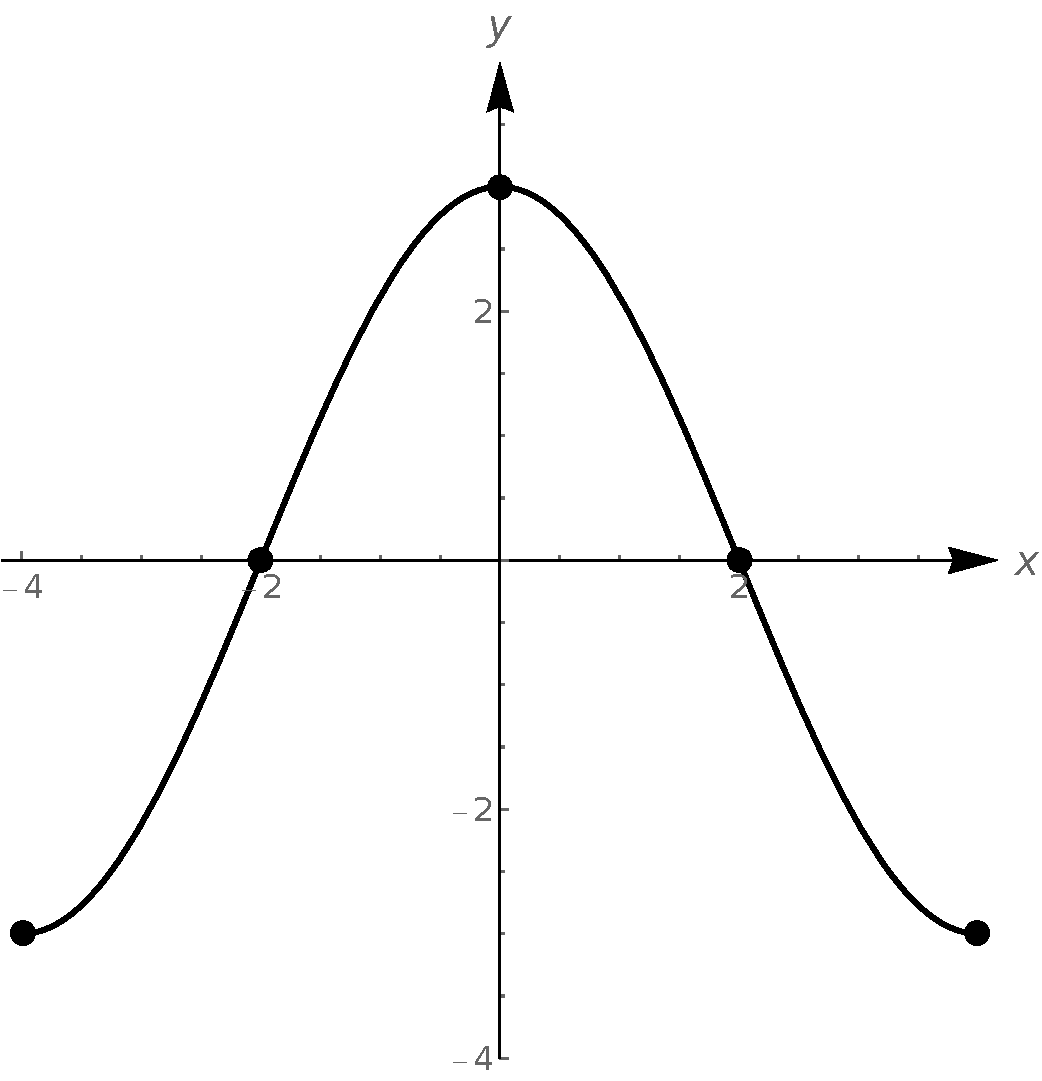
\includegraphics[width=0.3\textwidth]{fig_functions_21}
	\end{center}
	
	\begin{enumerate}
		
		\item  Find the domain of $f$.
		
		\item  Find the range of $f$.
		
		\item  Find the zeros of $f$.
		
		\item  Does $f$ appear to be even, odd, or neither?
		
		\item  List the intervals on which $f$ is increasing.
		
		\item  List the intervals on which $f$ is decreasing.
		
		\item  List the local maximums, if any exist.
		
		\item  List the local minimums, if any exist.
		
		
		\item  Find the maximum, if it exists.
		
		\item  Find the minimum, if it exists.
		
	\end{enumerate}
	
	
	\xhrulefill{gray}{2.5pt}Solution \xhrulefill{gray}{2.5pt}
	
	\begin{enumerate}
		
		\item  To find the domain of $f$, we proceed by projecting the graph to the $x$-axis, we see that the portion of the $x$-axis which corresponds to a point on the graph is everything from $-4$ to $4$, inclusive.  Hence,  $\dom\, f=[-4,4]$.
		
		\item  To find the range, we project the graph to the $y$-axis.  We see that the $y$-values from $-3$ to $3$, inclusive, constitute the range of $f$.  Hence, our answer is $[-3,3]$.
		
		\item  The zeros of $f$ are the $x$-coordinates of the $x$-intercepts of the graph of $y=f(x)$ which are $x=-2$ and $x=2$.
		
		\item The graph is symmetric about the $y$-axis, so $f$ is even.
		
		\item  As we move from left to right, the graph rises from $(-4,-3)$ to $(0,3)$. This means $f$ is increasing on the interval $[-4,0]$.  
		
		\item  As we move from left to right, the graph falls from $(0,3)$ to $(4,-3)$.  This means $f$ is decreasing on the interval $[0,4]$.  
		
		\item  The function has its only local maximum at $(0,3)$ so $f(0) = 3$ is the local maximal value.
		
		\item  There are no local minimums.  Why do $(-4, -3)$ and $(4, -3)$ not count?  Let us consider the point $(-4, -3)$ for a moment.  Recall that, in Definition~\ref{defmaxmin}, there needs to be an open interval $I$ which contains $x = -4$ such that $f(-4) < f(x)$ for all $x$ in $I$ different from $-4$.  But if we put an open interval around $x= -4$ a portion of that interval will lie outside of the domain of $f$.  Because we are unable to fullfill the requirements of the definition for a local minimum, we cannot claim that $f$ has one at $(-4, -3)$.  The point $(4, -3)$ fails for the same reason.
		
		\item  The maximum value of $f$ is the largest $y$-coordinate which is $3$.
		
		\item  The minimum value of $f$ is the smallest $y$-coordinate which is $-3$.
		
	\end{enumerate}
	
\end{example}
\fi




\subsection{Transformations}
\label{sec_transformations}

We may change or transform the graphs of functions by making certain modifications to their formulas. The transformations we will study fall into three broad categories:  shifts, reflections and scalings.  Suppose the graph in Figure~\ref{fig_functions_22} is the complete graph of a function $f$.

\begin{figure}[h!]
	\begin{center}
			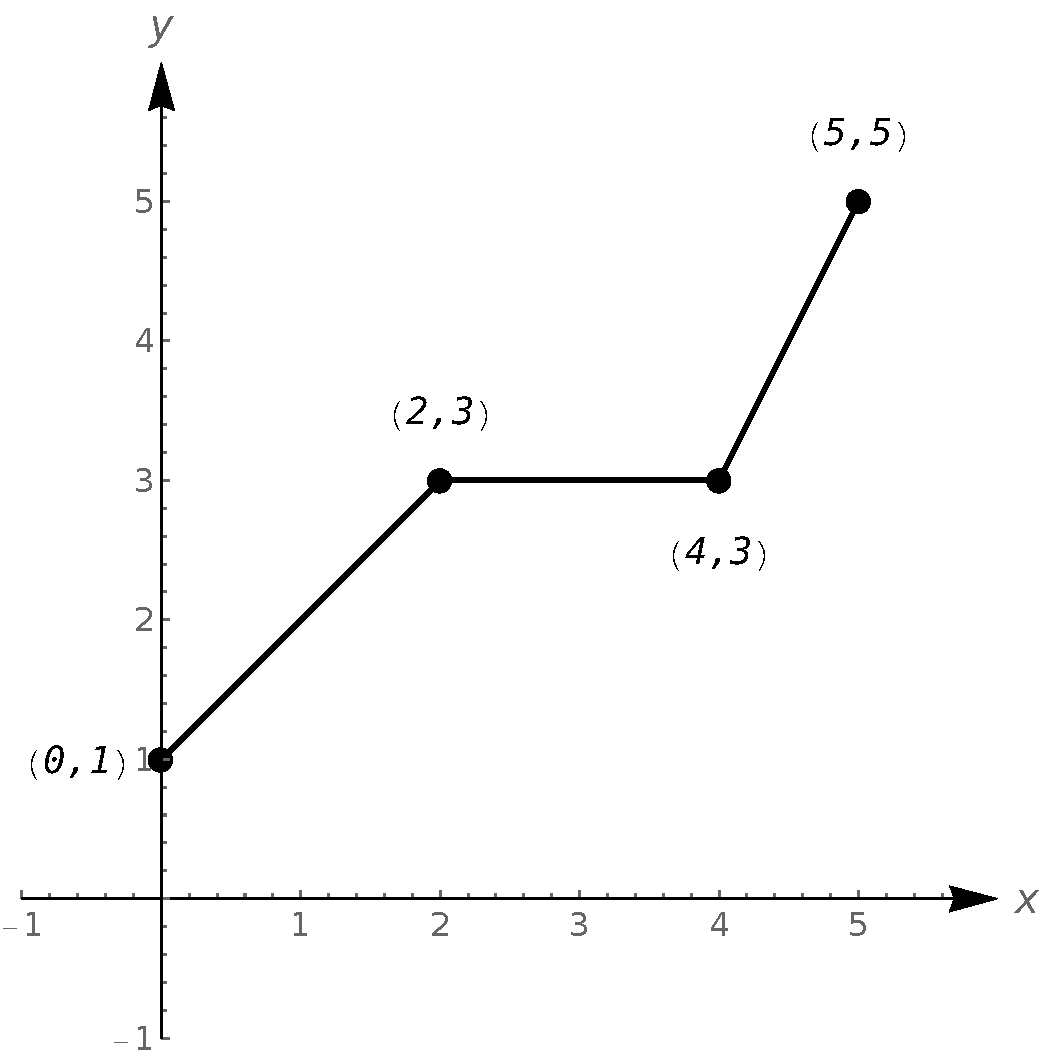
\includegraphics[width=0.3\textwidth]{fig_functions_22}
	\caption{The graph of $y=f(x)$.}
	\label{fig_functions_22}
	\end{center}
\end{figure}


Suppose we wanted to graph the function defined by the formula $g_1(x) = f(x) + 2$.  In order to graph $g_1$, we need to graph the points $(x,g_1(x))$.  For example, using the points indicated on the graph of $f$, we can make the following table.

\[ \begin{array}{c|cc}  


x  & f(x) & g_1(x)=f(x)+2  \\ \hline\hline
0  & 1 & 3 \\  
2  & 3 &  5  \\  
4  & 3 &  5 \\  
5  & 5 &  7  \\  

\end{array} \] 

Hence, to obtain the graph of $g_1$, we just add $2$ to the $y$-coordinate of each point on the graph of $f$ (Figure~\ref{fig_functions_23a}).  Geometrically, we are `shifting the graph up $2$ units'.  It is important to note that the domain of $f$ and the domain of $g$ are the same, but that the range of $f$ is $[1,5]$ while the range of $g_1$ is $[3,7]$.  In general, \textbf{shifting a function vertically} (\textit{verticale verschuiving}) like this will leave the domain unchanged, but could very well affect the range.
\index{function ! vertical shift}\index[aut]{functie ! verticale verschuiving}
%\index{shift}\index[aut]{verschuiving}

You can easily imagine what would happen if we wanted to graph the function $j_1(x) = f(x) - 2$.  Geometrically, we would then shift the graph down $2$ units (Figure~\ref{fig_functions_23b}). 

\begin{figure}[H]
\centering
%\raisebox{0.5cm}{
\centerline{
\subfigure[$y=g_1(x)=f(x)+2$\label{fig_functions_23a}]{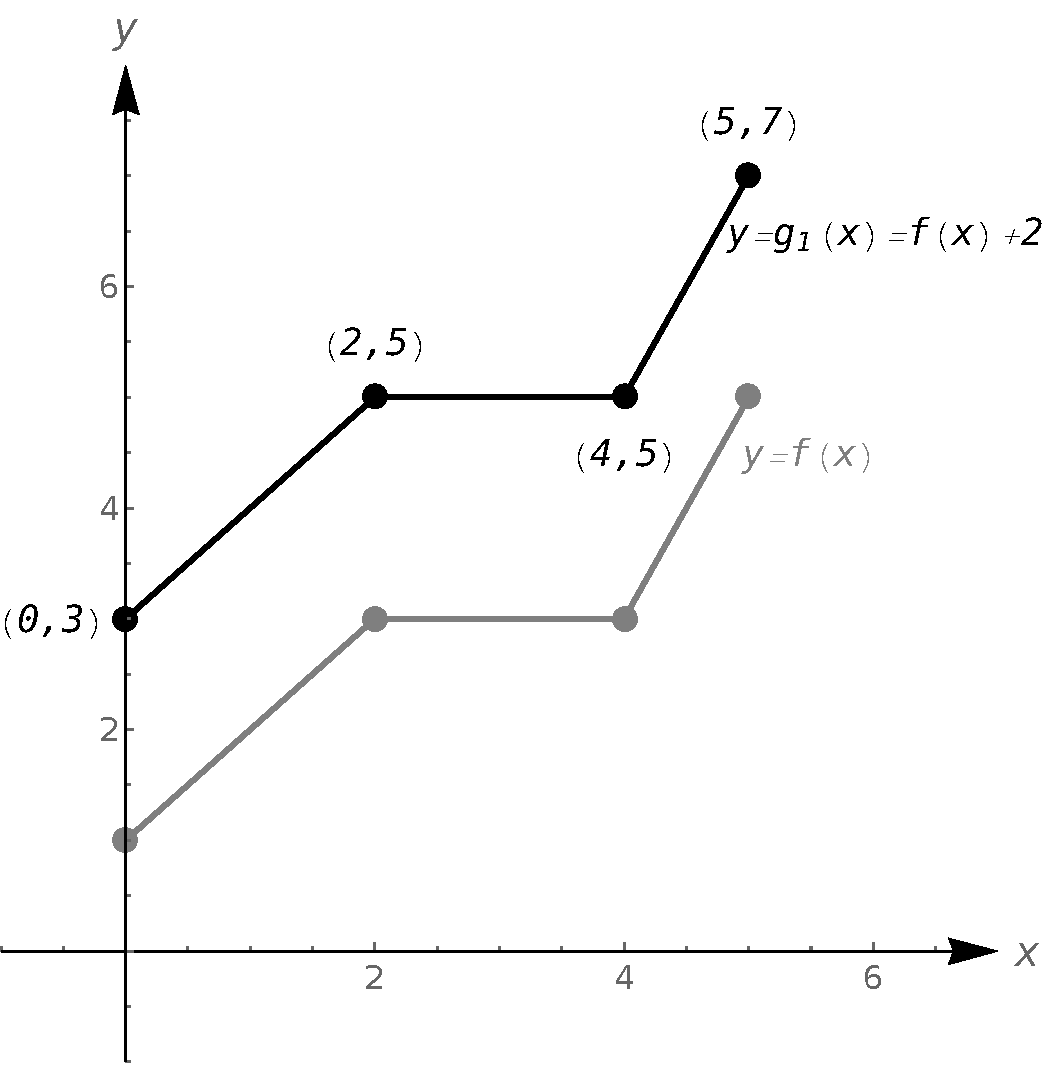
\includegraphics[width=0.4\textwidth]{fig_functions_23a}}
\hspace{0.1cm}
\subfigure[$y=j_1(x)=f(x)-2$ \label{fig_functions_23b}]{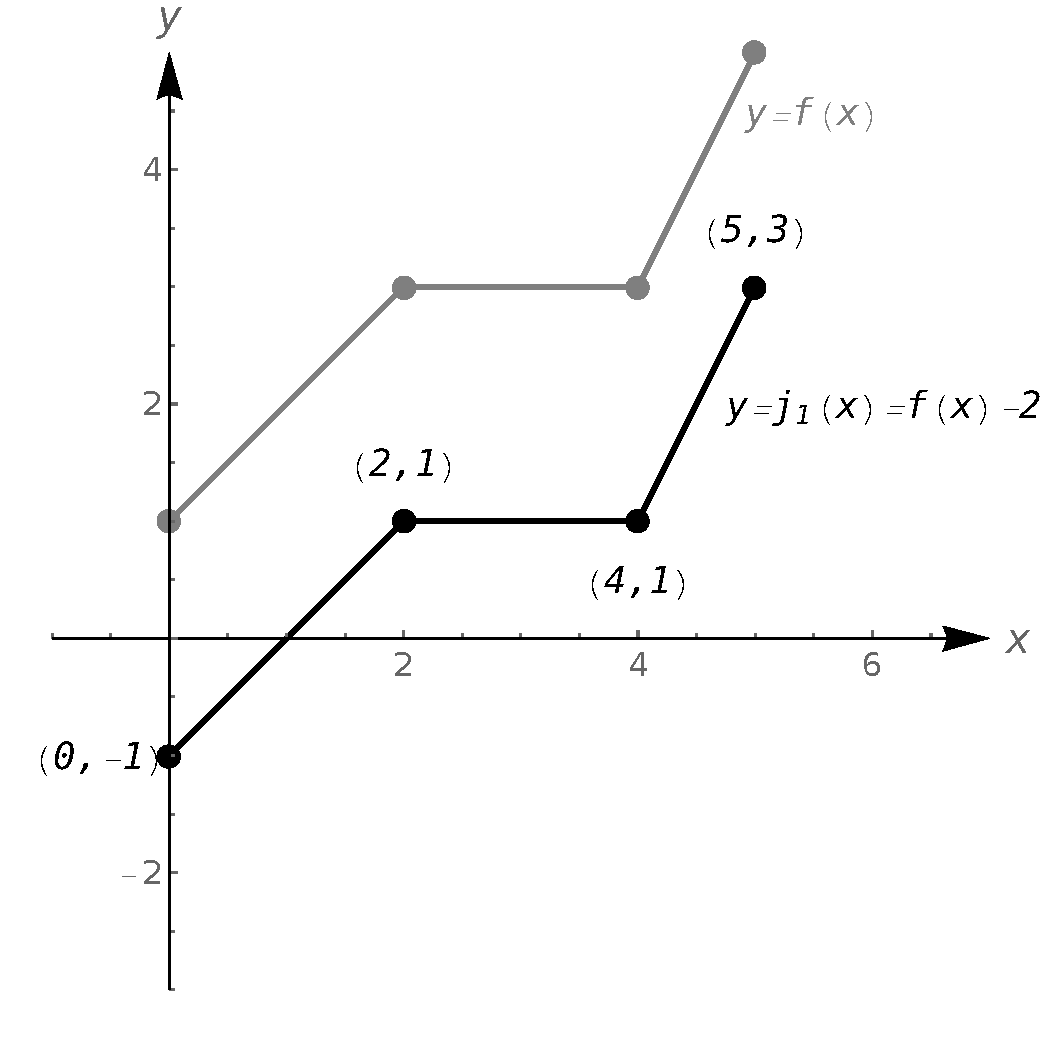
\includegraphics[width=0.4\textwidth]{fig_functions_23b}}
}
\caption{Vertical shifts of the graph of $y=f(x)$: two units up (a) and down (b). }
\end{figure}

Now, what happens if we add to or subtract from the input of the function?  For instance, suppose we wanted to graph $g_2(x) = f(x+2)$.  We know, for instance, $f(0) = 1$.  To determine the corresponding point on the graph of $g_2$, we need to figure out what value of $x$ we must substitute into $g_2(x) = f(x+2)$ so that the quantity $x+2$, works out to be $0$.  Solving $x+2=0$ gives $x=-2$,  so  $(-2,1)$ is on the graph of $g_2$.  Continuing in this fashion, we get the following table.

\[ \begin{array}{r|rcl}  
x & g_2(x)&=&f(x+2)  \\ \hline\hline
-2 & g_2(-2)&=&f(0) = 1   \\  
0  &  g_2(0)&=&f(2) = 3   \\  
2   & g_2(2)&=&f(4) = 3 \\  
3  & g_2(3)&=&f(5) = 5   \\  

\end{array} \] 

In summary, the points $(0,1)$, $(2,3)$, $(4,3)$ and $(5,5)$ on the graph of $y=f(x)$ give rise to the points  $(-2,1)$, $(0,3)$, $(2,3)$ and $(3,5)$ on the graph of $y=g_2(x)$, respectively.  In general, if $(a,b)$ is on the graph of $y=f(x)$, then $(a-2,b)$ is on the graph of $y=g_2(x)$. The point $(a-2,b)$ is exactly $2$ units to the left of the point $(a,b)$ so the graph of $y=g_2(x)=f(x+2)$ is obtained by shifting the graph $y=f(x)$ to the left $2$ units (Figure~\ref{fig_functions_24a}).

Note that while the ranges of $f$ and $g_2$ are the same, the domain of $g_2$ is $[-2,3]$ whereas the domain of $f$ is $[0,5]$.  In general, when we \textbf{shift the graph horizontally} (\textit{horizontale verschuiving}), the range will remain the same, but the domain could change.  Similarly, if we set out to graph $j_2(x) = f(x-2)$, we would  effect a shift to the right $2$ units (Figure~\ref{fig_functions_24b}).
\index{function ! horizontal shift}\index[aut]{functie ! horizontale verschuiving}

\begin{figure}[H]
\centering
%\raisebox{0.5cm}{
\centerline{
\subfigure[$y=g_2(x)=f(x+2)$\label{fig_functions_24a}]{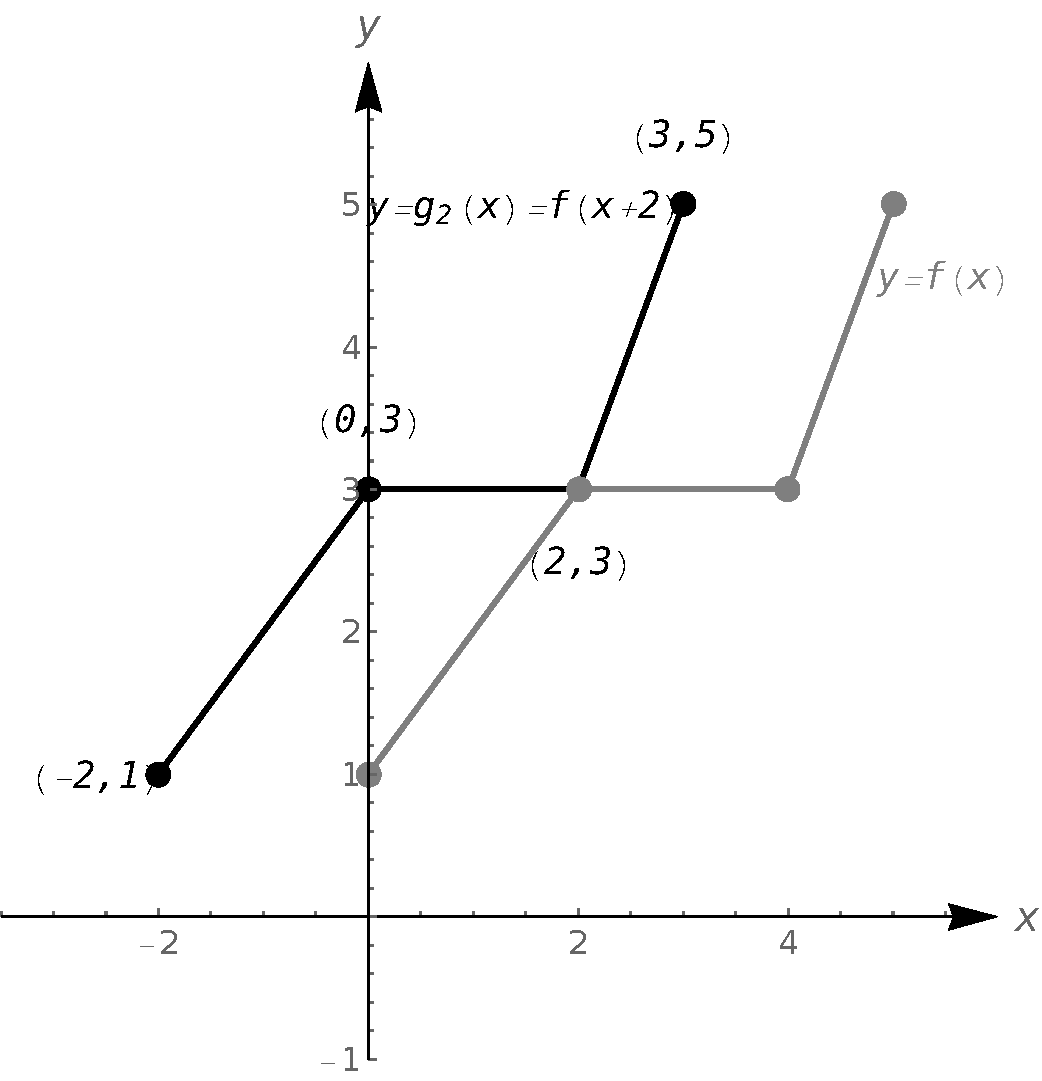
\includegraphics[width=0.4\textwidth]{fig_functions_24a}}
\hspace{0.1cm}
\subfigure[$y=j_2(x)=f(x-2)$ \label{fig_functions_24b}]{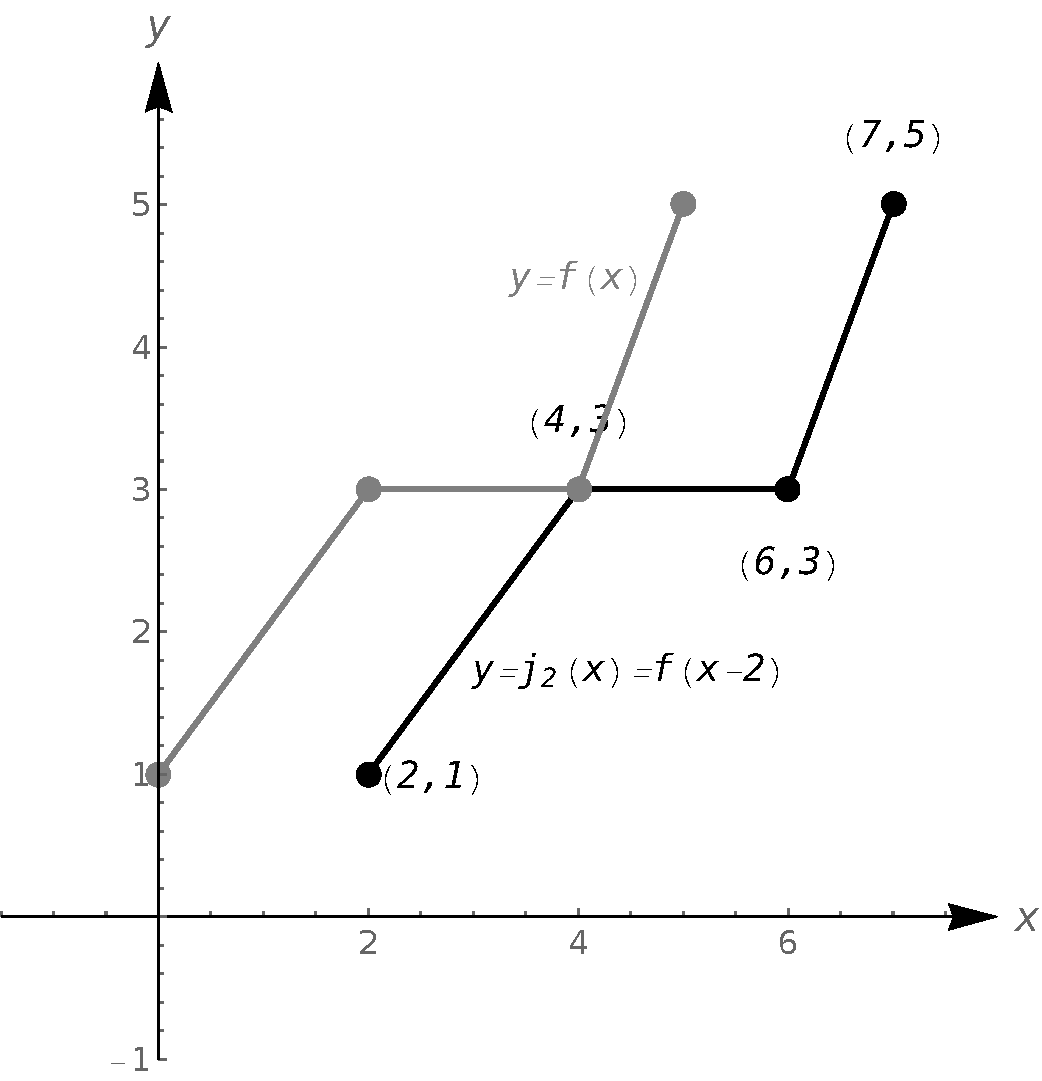
\includegraphics[width=0.4\textwidth]{fig_functions_24b}}
}
\caption{Horizontal shifts of the graph of $y=f(x)$: two units to the left (a) and right (b). }
\end{figure}


We now turn our attention to \textbf{reflections} (\textit{spiegeling}). We know from Section \ref{CartesianPlane} that the graph of $y=-f(x)$ is the graph of $f$ reflected across the $x$-axis (Figure~\ref{fig_functions_25a}).  Similarly, the graph of $y=f(-x)$ is the graph of $f$ reflected across the $y$-axis (Figure~\ref{fig_functions_25b}).  
\index{function ! reflection}\index[aut]{functie ! spiegeling}


\begin{figure}[t]
\centering
%\raisebox{0.5cm}{
\centerline{
\subfigure[$y=g_3(x)=-f(x)$\label{fig_functions_25a}]{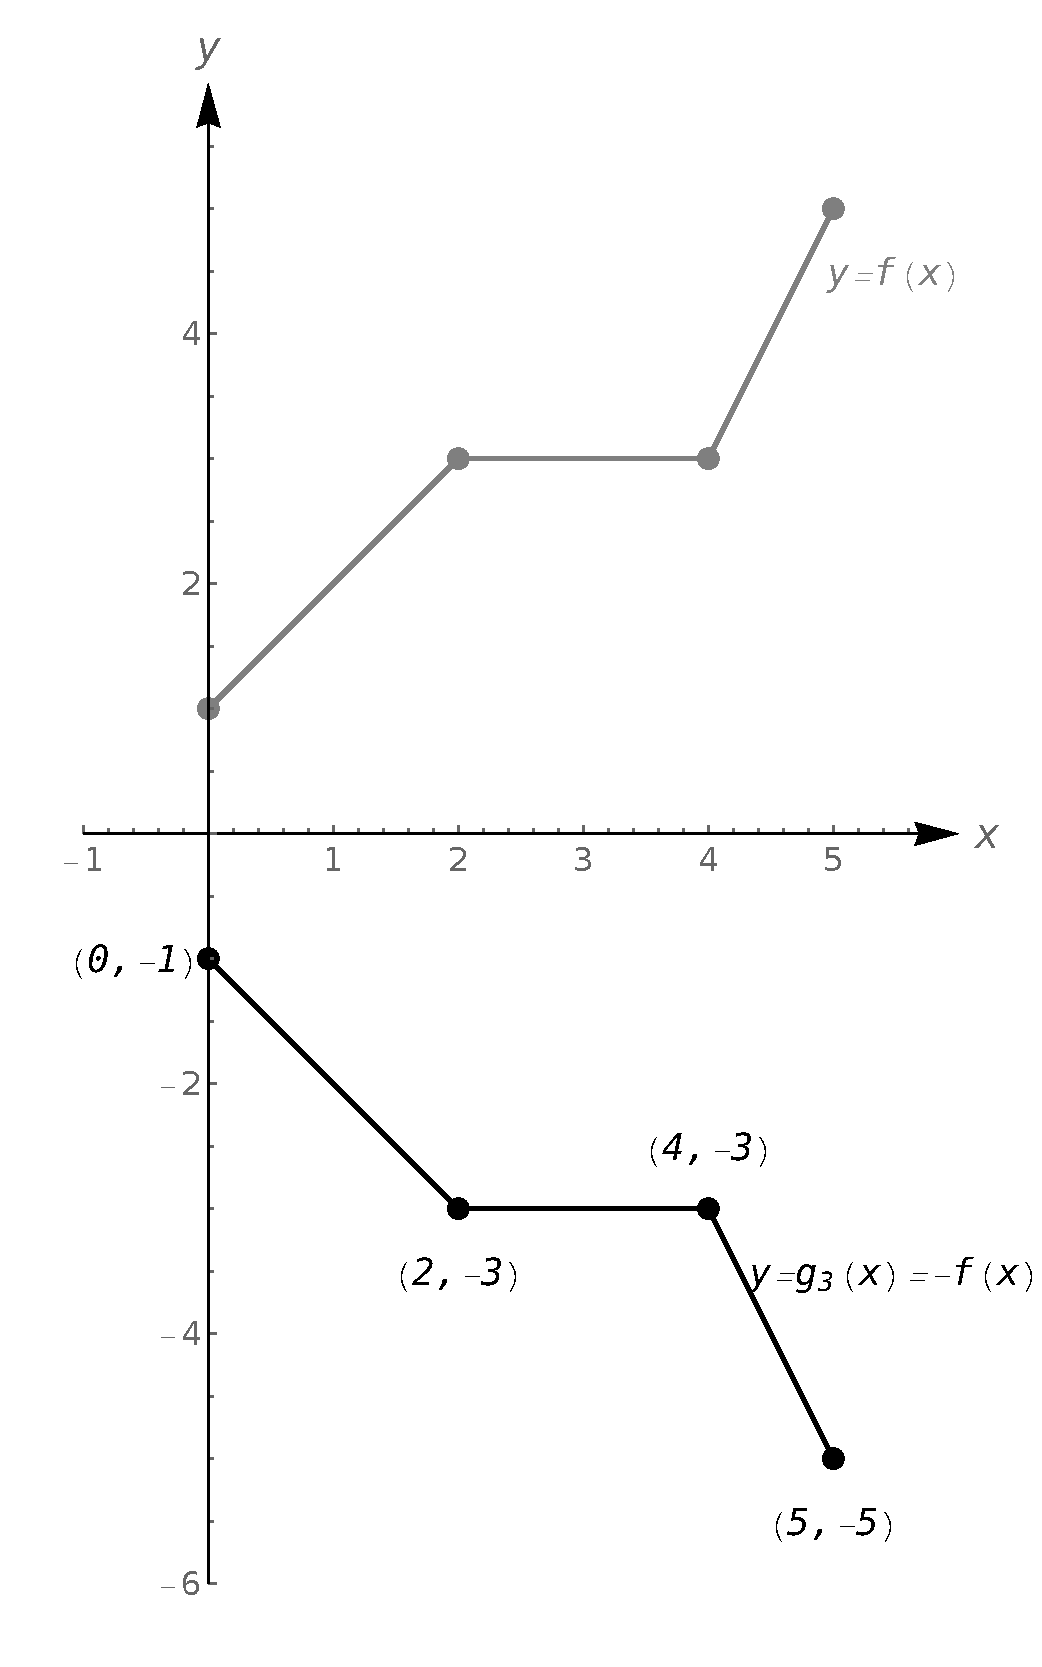
\includegraphics[width=0.4\textwidth]{fig_functions_25a}}
\hspace{0.1cm}
\subfigure[$y=j_3(x)=f(-x)$ \label{fig_functions_25b}]{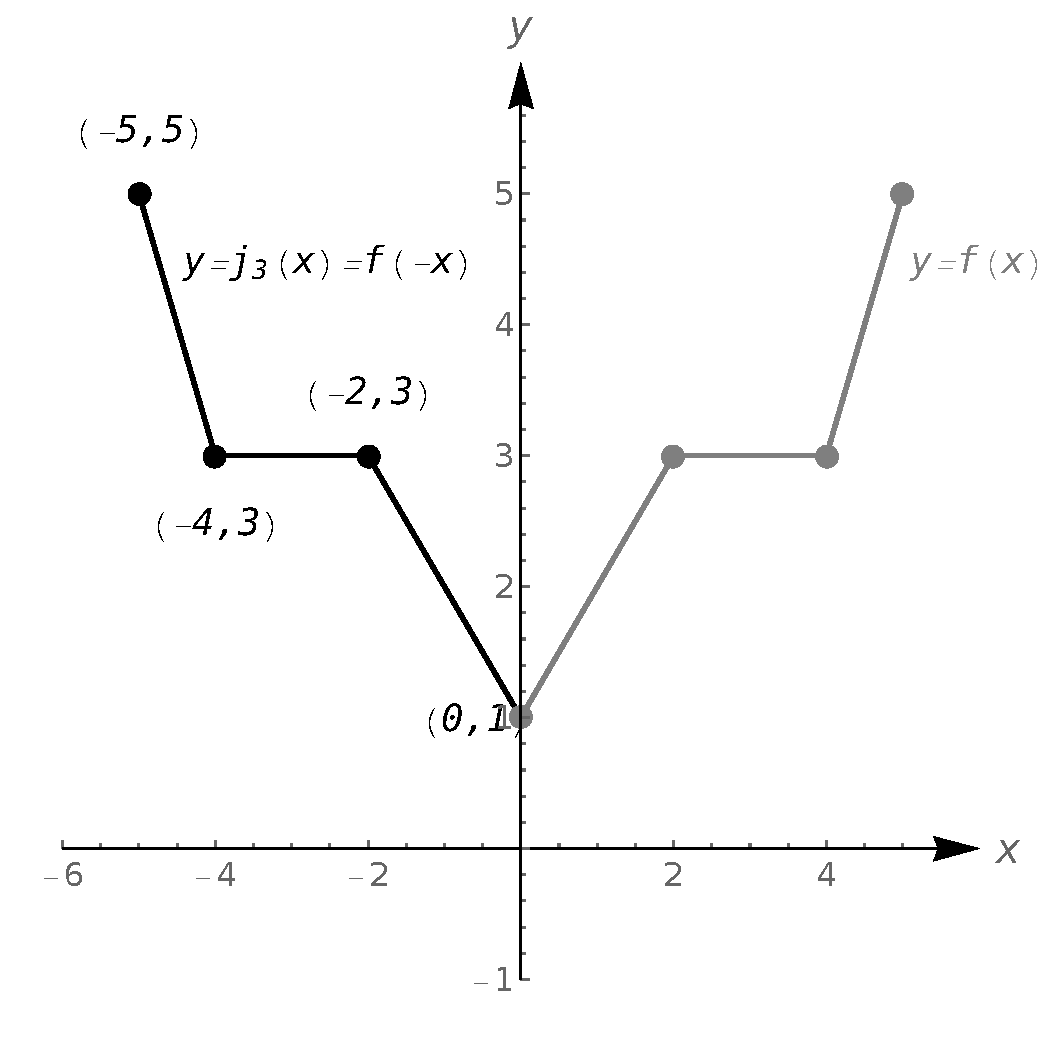
\includegraphics[width=0.4\textwidth]{fig_functions_25b}}
}
\caption{Reflections of the graph of $y=f(x)$: across $x$-axis (a) and $y$-axis (b). }
\end{figure}

Finally, we turn our attention to our last class of transformations known as \textbf{scalings} (\textit{schaling}).  A thorough discussion of scalings can get complicated because they are not as straightforward as the previous transformations.  The transformations covered so far are known as \textbf{rigid transformations} (\textit{directe isometrie}) because they do not change the shape of the graph, only its position and orientation in the plane.  If, however, we wanted to make a new graph twice as tall as a given graph, we would be changing the shape of the graph. This type of transformation is called \textbf{non-rigid} (\textit{indirecte isometrie}).  Not only will it be important for us to differentiate between modifying inputs versus outputs, we must also pay close attention to the magnitude of the changes we make.
\index{function ! scaling}\index[aut]{functie ! schaling}
\index{function ! rigid transformation} \index[aut]{functie ! directe isometrie}
\index{function ! non-rigid transformation} \index [aut]{functie ! indirecte isometrie}

Suppose we wish to graph the function $g_4(x) =2 f(x)$. From its graph, we can build a table of values for $g_4$ as before.
\begin{center}
\begin{tabular}{c|cc}  
$x$  & $f(x)$ & $g_4(x)=2f(x)$  \\ \hline\hline
0  & 1 & 2 \\  
2  & 3 &  6  \\  
4  & 3 &  6 \\  
5  & 5 &  10  \\
\end{tabular} 
\end{center}

If $(a,b)$ is on the graph of $f$, then $(a,2b)$ is on the graph of $g_4$.  In other words, to obtain the graph of $g_4$, we multiply all of the $y$-coordinates of the points on the graph of $f$ by $2$.  This is known as a vertical scaling by a factor of $2$ (Figure~\ref{fig_functions_26a}). Likewise, if we wish to graph $y = \frac{1}{2} f(x)$, we multiply all of the $y$-coordinates of the points on the graph of $f$ by $\frac{1}{2}$.  This creates a vertical scaling by a factor of $\frac{1}{2}$ (Figure~\ref{fig_functions_26b}).

\begin{figure}
\centering
%\raisebox{0.5cm}{
\centerline{
\subfigure[$y=g_4(x)=2f(x)$\label{fig_functions_26a}]{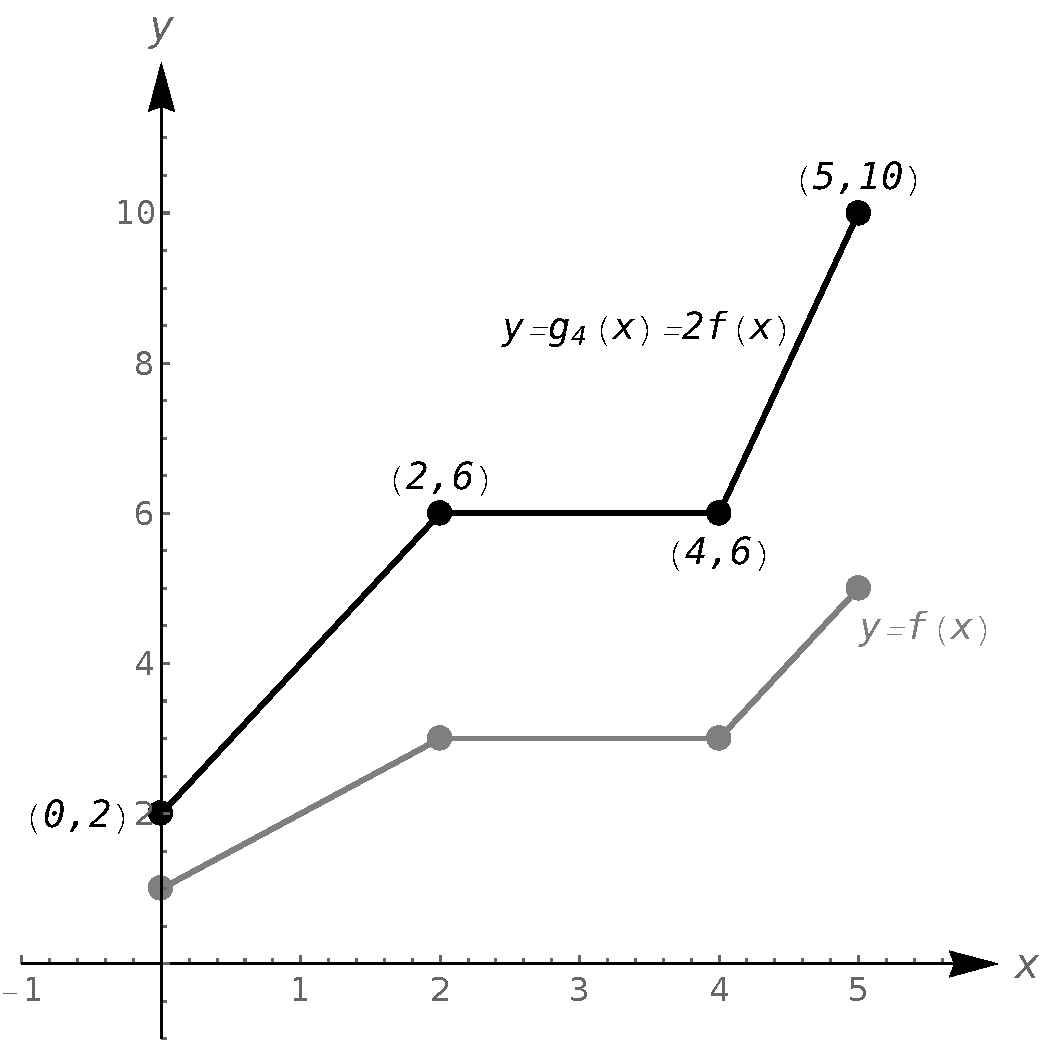
\includegraphics[width=0.4\textwidth]{fig_functions_26a}}
\hspace{0.1cm}
\subfigure[$y=j_4(x)=\frac{1}{2}f(x)$ \label{fig_functions_26b}]{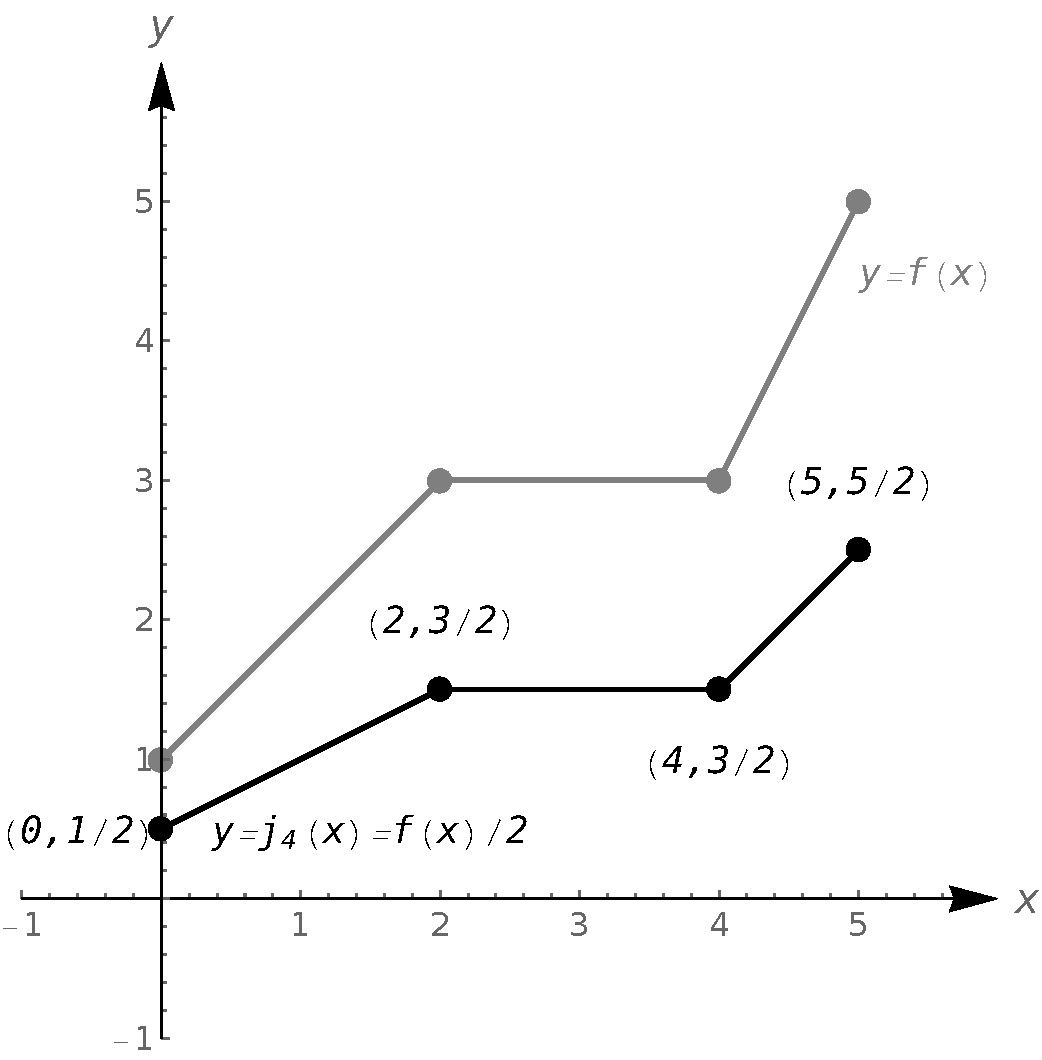
\includegraphics[width=0.4\textwidth]{fig_functions_26b}}
}
\caption{Vertical scalings of the graph of $y=f(x)$: stretching by a factor 2 (a);  shrinking by a factor 1/2 (b). }
\end{figure}

In general, suppose $f$ is a function and $a>0$, then to obtain the graph of $y=a f(x)$, we have to vertically scale the graph of $f$  by a factor of $a$. 

\begin{itemize}

\item If $a > 1$, we say the graph of $f$ has undergone a \textbf{vertical stretching (expansion, dilation)} by a factor of $a$. 

\item If $0 < a < 1$, we say the graph of $f$ has undergone a \textbf{vertical shrinking (compression, contraction)} by a factor of $\frac{1}{a}$.
\index{function ! vertical stretching (expansion, dilation)} 
\index{function ! vertical shrinking (compression, contraction)}
\end{itemize}

In terms of inputs and outputs,  multiplying the outputs from a function by positive number $a$ causes the graph to be vertically scaled by a factor of $a$.  It is natural to ask what would happen if we multiply the inputs of a function by a positive number.  This leads us to our last transformation.


Suppose we want to graph $g_5(x) = f(2x)$.   If we want to determine the point on $g_5$ which corresponds to the point $(2,3)$ on the graph of $f$,  we set $2x =2 $ so that $x=1$.  Substituting $x=1$ into $g_5(x)$, we obtain $g_5(1) = f(2 \cdot 1) = f(2) = 3$, so that $(1,3)$ is on the graph of $g_5$. Continuing in this fashion, we obtain the following table.   

\begin{center}
\begin{tabular}{r|rcl}  
$x$ & $g_5(x)$&=&$f(2x)$  \\ \hline\hline
0 & $g_5(0)$&=&$f(0) = 1$   \\  
1  &  $g_5(1)$&=&$f(2) = 3$   \\  
2   & $g_5(2)$&=&$f(4) = 3$ \\  
$\frac{5}{2}$  & $g_5(5/2)$&=&$f(5)$ = 5   
\end{tabular} 
\end{center}



In general, if $(a,b)$ is on the graph of $f$, then $\left(\frac{a}{2}, b\right)$ is on the graph of $g$.  This results in a horizontal scaling by a factor of $\frac{1}{2}$ (Figure~\ref{fig_functions_27a}). If, on the other hand, graphing $y = f\left( \frac{1}{2} x\right)$, results in a horizontal scaling by a factor of $2$ (Figure~\ref{fig_functions_27b}).







In general, suppose $f$ is a function and $b>0$, then to obtain the  graph of $y= f(bx)$, we have to horizontally scale the graph of $f$ by a factor of $\frac{1}{b}$. 

\begin{itemize}

\item If $0 < b < 1$, we say the graph of $f$ has undergone a \textbf{horizontal stretching (expansion, dilation)} by a factor of $\frac{1}{b}$. 
\item If $b>1$, we say the graph of $f$ has undergone a \textbf{horizontal shrinking (compression, contraction)} by a factor of $b$.
\end{itemize}

\begin{figure}[h]
\centering
%\raisebox{0.5cm}{
\centerline{
\subfigure[$y=g_5(x)=f(2x)$\label{fig_functions_27a}]{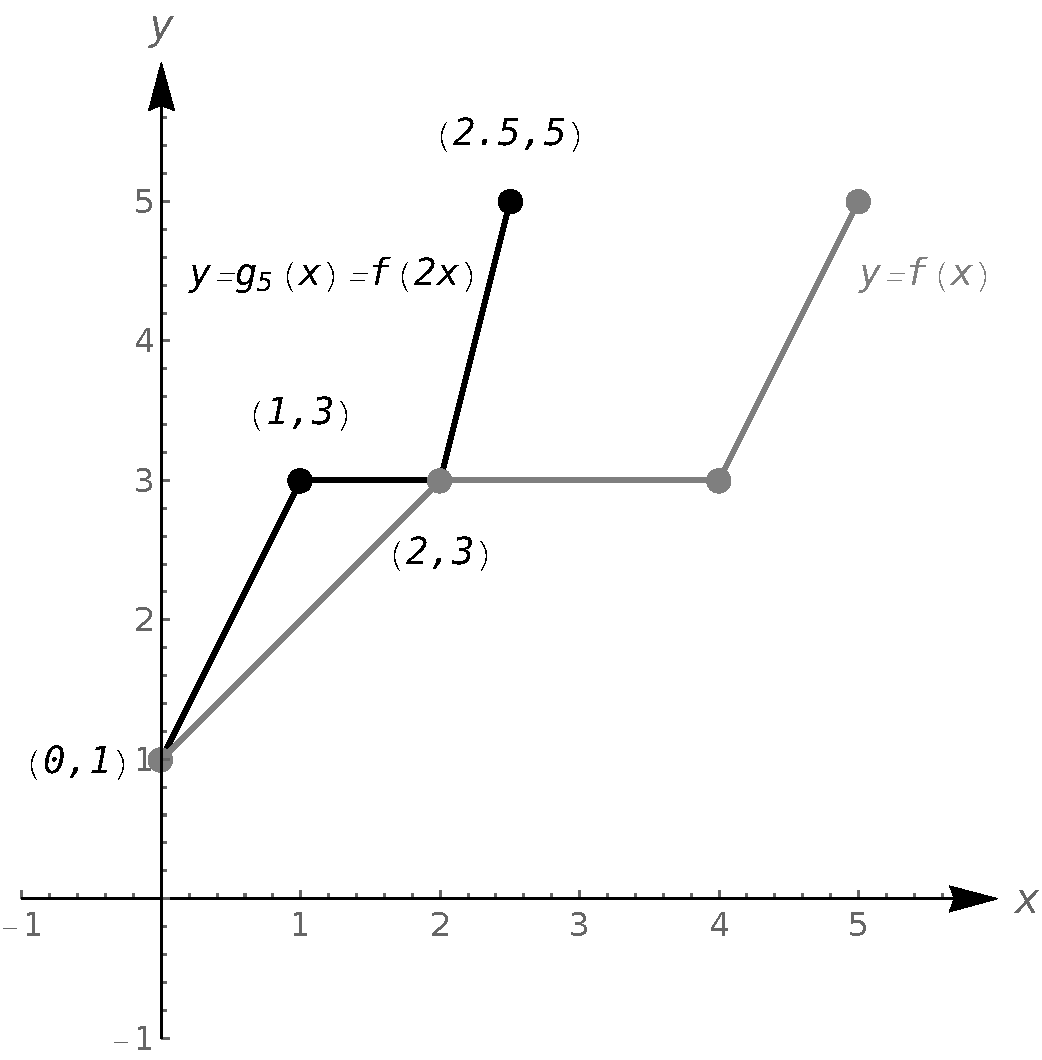
\includegraphics[width=0.4\textwidth]{fig_functions_27a}}
\hspace{0.1cm}
\subfigure[$y=j_5(x)=f(\frac{x}{2})$ \label{fig_functions_27b}]{\includegraphics[width=0.4\textwidth]{fig_functions_27b}}
}
\caption{Horizontal scalings of the graph of $y=f(x)$: shrinking by a factor 2 (a);  streching by a factor 1/2 (b). }
\end{figure}
\pagebreak


\begin{example}
 Below is the complete graph of $y = f(x)$.  Use it to graph 
 $$g(x) = \dfrac{4-3\,f(1-2x)}{2}.$$


	\begin{center}
			\includegraphics[width=0.3\textwidth]{fig_functions_28}
	\end{center}

\xhrulefill{gray}{2.5pt}Solution \xhrulefill{gray}{2.5pt}

We track the five key points $(-4,-3)$, $(-2,0)$, $(0,3)$, $(2,0)$ and $(4,-3)$ indicated on the graph of $f$ to their new locations.  We first rewrite $g(x)$ as
 $$g(x) = -\frac{3}{2}f(-2x+1) +2\,.$$
Let us first focus on $f(-2x+1)$. To get from $f(x)$ to $f(-2x+1)$, we need a horizontal shift with one unit, i.e.\ $f(x+1)$, followed by a horizontal shrinking by a factor of 2, i.e.\ $f(2x+1)$, followed on its turn by a reflection across the $y$-axis. So,  we set $-2x+1$ equal to the $x$-coordinates of the key points and solve.  For example, solving $-2x+1 = -4$, we get $x = \frac{5}{2}$.  We summarize the results in the table below. 

\renewcommand{\arraystretch}{1.5}
\[  \begin{array}{c|ccccc}  

a &-4&-2&0&2&4\\\hline
x = \frac{a-1}{2}&\frac{5}{2}&\frac{3}{2}&\frac{1}{2}&-\frac{1}{2}&-\frac{3}{2}
\end{array} \]
\renewcommand{\arraystretch}{1}


Next, we take each of the $x$ values and substitute them into $g(x) = -\frac{3}{2}f(-2x+1) +2$ to get the corresponding $y$-values.  Substituting  $x=\frac{5}{2}$, and using the fact that $f(-4)=-3$, we get \[g\left(\frac{5}{2}\right) = -\frac{3}{2}f\left(-2\left(\frac{5}{2}\right) +1\right) +2 = -\frac{3}{2} f(-4) + 2 = -\frac{3}{2}(-3) + 2 = \frac{9}{2} + 2 = \frac{13}{2}.\] 
We see that the output from $f$ is first multiplied by $-\tfrac{3}{2}$.  Thinking of this as a two step process, multiplying by $\tfrac{3}{2}$ and then by $-1$, we have  a vertical stretching by a factor of $\tfrac{3}{2}$ followed by a reflection across the $x$-axis.  Adding $2$ results in a vertical shift up $2$ units.  Continuing in this manner, we get the following table.

\renewcommand{\arraystretch}{1.5}
\[  \begin{array}{c|ccccc}  
 x &  \frac{5}{2}&\frac{3}{2}&\frac{1}{2}&-\frac{1}{2}&-\frac{3}{2}\\ \hline
 g(x)& \frac{13}{2}  & 2 & - \frac{5}{2}  & 2  & \frac{13}{2}  \\ 
\end{array} \]
\renewcommand{\arraystretch}{1}


To graph $g$, we plot each of the points in the table above and connect them in the same order and fashion as the points to which they correspond (Figure~\ref{fig_functions_29b}).  The reader is strongly encouraged to graph the series of functions which shows the gradual transformation of the graph of $f$ into the graph of $g$.  

\begin{figure}[H]
    \centering
    \centerline{
        \subfigure[$f(x)$]{\includegraphics[width=0.4\textwidth]{fig_functions_29a}}
        \hspace{0.1cm}
        \subfigure[$g(x) = \frac{4-3 f(1-2x)}{2}$\label{fig_functions_29b}]{\includegraphics[width=0.4\textwidth]{fig_functions_29b}}
    }
	\caption{The graph of the original function $f(x)$ (a), alongside the transformed function $g(x)$ (b).}
\end{figure}

\end{example}



\subsection{Piecewise-defined functions}\label{stuksgewijs_gedef_functies}
In many applications, one will encounter functions that are defined on a sequence of intervals. Such functions are referred to as \textbf{piecewise-defined functions}, or \textbf{piecewise functions} (\textit{stuksgewijze functie}) for short. For instance, 
\begin{equation}
\label{ex_piece}
f(x) = \left\{\begin{array}{rcl} 
(x+1)^2,  & \mbox{if} & x<-1,\\
-x, & \mbox{if} & -1\leq x<1,\\
\sqrt{x-1}, & \mbox{ if} & x\geq 1,
\end{array}\right. 
\end{equation}
is a piecewise function. Its graph is given in Figure~\ref{fig_functions_30}
\index{function ! piecewise}\index[aut]{functie ! stuksgewijs}


\begin{figure}[h!]
	\begin{center}
			\includegraphics[width=0.3\textwidth]{fig_functions_30}
	\caption{The graph of Equation~\eqref{ex_piece}.}
	\label{fig_functions_30}
	\end{center}
\end{figure}


\subsection{Function families}
Throughout the remainder of this course we will focus our attention on the so-called \textbf{elementary functions} (\textit{elementaire functie}), which are functions that are  compositions of a finite number of arithmetic operations, exponentials, logarithms, constants, and solutions of algebraic equations. Two important families can be distinguished among the elementary functions, namely the \textbf{algebraic} (\textit{algebra\"ische}) and \textbf{transcendental functions} (\textit{transcendente functie}).
\index{function ! elementary}\index[aut]{functie ! elementaire}
\index{function ! algebraic}\index[aut]{functie ! algebraïsche}
\index{function ! transcendental}\index[aut]{functie ! transcendente}

An algebraic function is a function that can be defined as the root of a polynomial equation. Quite often algebraic functions are algebraic expressions using a finite number of terms, involving only the algebraic operations addition, subtraction, multiplication, division, and raising to a fractional power. Examples of such functions are:
\begin{itemize}
\item power functions, e.g. $f(x)=2x^3$,
\item polynomial functions, e.g. $f(x)=1+x+x^3$,
\item rational functions, e.g.
$$
f(x)=\dfrac{1+x}{1+x+x^3}\,,
$$
\item irrational functions, e.g. $f(x)=\sqrt{1+x+x^3}$, 
\item and any compositions thereof, e.g.
$$
f(x)=\dfrac{1+x}{\sqrt{1+x+x^3}}\,.
$$
\end{itemize}

A transcendental function is a function that does not satisfy a polynomial equation, in contrast to an algebraic function. In other words, a transcendental function transcends algebra in that it cannot be expressed in terms of a finite sequence of the algebraic operations of addition, multiplication, and root extraction. Examples of transcendental functions include
\begin{itemize} 
\item exponential functions, e.g. $f(x)=2^x$,
\item logarithmic functions, e.g. $f(x)=\ln(x)$,
\item trigonometric functions, e.g. $f(x)=\sin(x)$,
\ifcourse 

 \item hyperbolic functions, e.g. $f(x)=\sinh(x)$,
 
 \fi
\item and most compositions thereof, e.g.
$$
f(x)=\dfrac{2^x}{\sin(x)}\,.
$$
\end{itemize}

Algebraic and transcendental functions are studied in detail in Chapter~\ref{chap_algebraic} and \ref{chap_trans}, respectively. 




\section{Absolute value functions}\label{abs_functies}
\subsection{Definition and properties}
Throughout this course we adopt the following definition of the absolute value.
\begin{definition}[Absolute value]

\label{absolutevalue}

The \index{absolute value}\index[aut]{absolute waarde} \textbf{absolute value} (\textit{absolute waarde}) of a real number $x$, denoted $|x|$, is given by
\ifcalculus\vspace*{-0.5cm}\fi
\[ |x| = \left\{ \begin{array}{rcl} -x, & \mbox{if} & x < 0,  \\ x, & \mbox{if} & x \geq 0. \\ \end{array} \right.\]
\ifcalculus\vspace*{-0.5cm}\fi
\end{definition}

In this definition, we define $|x|$ using a piecewise-defined function. Other ways to define the absolute value are that $|x|$ is the distance from the real number $x$ to $0$ on the number line, or by the equation $|x| = \sqrt{x^2}$. We first remind ourselves of the properties of the absolute value.

Let $a$, $b$ and $x$ be real numbers and let $n$ be an integer.  Then the following arithmetic properties hold.
\begin{itemize}

\item \textbf{Product rule:} $$|ab|= |a||b|,$$

\item \textbf{Power rule:} $$\left| a^{n} \right| = |a|^{n},$$ whenever $a^{n}$ is defined,

\item \textbf{Quotient rule:} $$\left| \dfrac{a}{b} \right| = \dfrac{|a|}{|b|},$$ provided $b \neq 0$.

\end{itemize}

Besides, we have that $|x| = 0$ if and only if $x = 0$, and 

\begin{itemize}

\item  for $c > 0$, $|x| = c$ if and only if $x = c$ or $-x = c$,

\item  for $c < 0$, $|x| = c$ has no solution.

\end{itemize}


\ifcourse
\ifanalysis

Finally, we have the following important theorem.

\begin{theorem} [The triangle inequality] \label{thmtype:1.1.1}
If $a$ and $b$ are any two real numbers$,$ then
\begin{equation} \label{eq:1.1.3}
|a+b|\le |a|+|b|.
\end{equation}
\end{theorem}

%  There are four possibilities:
% \begin{enumerate}
% \item % (a)
% If $a\ge0$ and $b\ge0$, then $a+b\ge0$, so
% $|a+b|=a+b=|a|+|b|$.
% \item % (b)
% If $a\le0$ and $b\le0$, then $a+b\le0$, so
% $|a+b|=-a+(-b)=|a|+|b|$.
% \item % (c)
%  If $a \ge 0$ and $b \le 0$, then $a+b=|a|-|b|$.
% \item % (d)
%  If $a \le 0$  and $b  \ge 0$, then $a+b=-|a|+|b|$.
% \end{enumerate}
% Equation~\eqref{eq:1.1.3} holds in   cases (3) and (4), since
% \begin{equation}
% |a+b|=
% \begin{cases}
% |a|-|b|,& \text{ if } |a| \ge |b|,\\
% |b|-|a|,& \text{ if } |b| \ge |a|.
% \end{cases}
% \end{equation}

The triangle inequality appears in various forms in many contexts.
It is  the most important inequality in mathematics. We will use it often.


\fi
\fi




\ifcalculus
\begin{example}
	Solve each of the following equations.
	
	\begin{enumerate}
		\begin{multicols}{3}
			\item  $|3x-1| = 6$
			\item  $|x| = x^2-6$
			\item  $|x-2| + 1 = x$
		\end{multicols}
	\end{enumerate}
	
	\xhrulefill{gray}{2.5pt}Solution \xhrulefill{gray}{2.5pt}
	
	\begin{enumerate}
		
		\item  The equation  $|3x-1| = 6$ is of the form $|x| = c$ for $c>0$, so $|3x-1| = 6$ is equivalent to $3x-1=6$ or $3x-1 = -6$.  Solving the former, we arrive at $x = \frac{7}{3}$, and solving the latter, we get $x = -\frac{5}{3}$.  
		
		\item 	For $x < 0$, we have that $|x| = -x$, so for $x < 0$, the equation $|x| = x^2-6$ is equivalent to $-x = x^2-6$.  Rearranging this gives us $x^2+x-6 = 0$, or $(x+3)(x-2) = 0$.  We get $x = -3$ or $x=2$.  Since only $x=-3$ satisfies $x<0$, this is the answer we keep.
		
		 For $x \geq 0$, we have that $|x| = x$, so the equation $|x| = x^2-6$ becomes $x = x^2-6$.  From this, we get $x^2-x-6 =0$ or $(x-3)(x+2) = 0$.  Our solutions are $x=3$ or $x = -2$, and since only $x=3$ satisfies $x \geq 0$, this is the one we keep.  All together, our two solutions to $|x| = x^2-6$ are $x=-3$ and $x=3$.
		
		\item  To solve $|x-2| + 1 = x$, we first isolate the absolute value and get 
		\begin{equation}
		|x-2| = x-1\,.
		\label{exabs}
		\end{equation}
		Since we see $x$ both inside and outside of the absolute value, we break the equation into cases:   \[ |x-2| = \left\{ \begin{array}{rcl} -(x-2), & \mbox{if} & (x-2) < 0,  \\ (x-2), & \mbox{if} & (x-2) \geq 0. \\ \end{array} \right.\]
		
		Simplifying yields 
		\[ |x-2| = \left\{ \begin{array}{rcl} -x+2, & \mbox{if} & x < 2, \\ x-2, & \mbox{if} & x \geq 2. \\ \end{array} \right.\]
		
		So, for $x<2$, we have that $|x-2| = -x+2$ and Equation~\eqref{exabs} becomes $-x+2 = x-1$, which gives $x = \frac{3}{2}$.  Since this solution satisfies $x < 2$, we keep it.  Next, for $x \geq 2$, it holds that $|x-2| = x-2$, so Equation~\eqref{exabs} becomes $x-2 = x-1$.  Here, the equation reduces to $-2 = -1$, which signifies we have no solutions here.  Hence, our only solution is $x = \frac{3}{2}$.  
	\end{enumerate}
\end{example}
\fi


\ifvc
\begin{example}
Solve each of the following equations.

\begin{enumerate}
\begin{multicols}{3}
\item  $|3x-1| = 6$
\item  $|x| = x^2-6$
\item  $|x-2| + 1 = x$
\end{multicols}
\end{enumerate}

\xhrulefill{gray}{2.5pt}Solution \xhrulefill{gray}{2.5pt}

\begin{enumerate}

\item  The equation  $|3x-1| = 6$ is of the form $|x| = c$ for $c>0$, so $|3x-1| = 6$ is equivalent to $3x-1=6$ or $3x-1 = -6$.  Solving the former, we arrive at $x = \frac{7}{3}$, and solving the latter, we get $x = -\frac{5}{3}$.  

\item  The equation  $|x| = x^2-6$ presents us with some difficulty, since $x$ appears both inside and outside of the absolute value. Moreover, there are values of $x$ for which $x^2-6$ is positive, negative and zero, so we cannot use the equality properties without the risk of introducing extraneous solutions, or worse, losing solutions.  For this reason, we break equations like this into cases  by rewriting the term in absolute values, $|x|$, using Definition \ref{absolutevalue}.  

For $x < 0$, we have that $|x| = -x$, so for $x < 0$, the equation $|x| = x^2-6$ is equivalent to $-x = x^2-6$.  Rearranging this gives us $x^2+x-6 = 0$, or $(x+3)(x-2) = 0$.  We get $x = -3$ or $x=2$.  Since only $x=-3$ satisfies $x<0$, this is the answer we keep. For $x \geq 0$, we have that $|x| = x$, so the equation $|x| = x^2-6$ becomes $x = x^2-6$.  From this, we get $x^2-x-6 =0$ or $(x-3)(x+2) = 0$.  Our solutions are $x=3$ or $x = -2$, and since only $x=3$ satisfies $x \geq 0$, this is the one we keep.  All together, our two solutions to $|x| = x^2-6$ are $x=-3$ and $x=3$.

\item  To solve $|x-2| + 1 = x$, we first isolate the absolute value and get 
\begin{equation}
|x-2| = x-1\,.
\label{exabs}
\end{equation}
  Since we see $x$ both inside and outside of the absolute value, we break the equation into cases:   \[ |x-2| = \left\{ \begin{array}{rcl} -(x-2), & \mbox{if} & (x-2) < 0,  \\ (x-2), & \mbox{if} & (x-2) \geq 0. \\ \end{array} \right.\]

Simplifying yields 
\[ |x-2| = \left\{ \begin{array}{rcl} -x+2, & \mbox{if} & x < 2, \\ x-2, & \mbox{if} & x \geq 2. \\ \end{array} \right.\]

So, for $x<2$, we have that $|x-2| = -x+2$ and Equation~\eqref{exabs} becomes $-x+2 = x-1$, which gives $x = \frac{3}{2}$.  Since this solution satisfies $x < 2$, we keep it.  Next, for $x \geq 2$, it holds that $|x-2| = x-2$, so Equation~\eqref{exabs} becomes $x-2 = x-1$.  Here, the equation reduces to $-2 = -1$, which signifies we have no solutions here.  Hence, our only solution is $x = \frac{3}{2}$.  
\end{enumerate}
\end{example}
\fi


\subsection{Absolute value functions}
Next, we turn our attention to graphing \textbf{absolute value functions} (\textit{absolute waarde functie}). Our strategy in the next example is to make liberal use of Definition \ref{absolutevalue}. 

\begin{example}
Graph each of the following functions.  
\begin{enumerate}
\begin{multicols}{2}
\item  $f(x) = |x|$
\ifvc \item  $g(x) = |x-3|$\fi
\ifcourse \item  $h(x) = \dfrac{|x|}{x}$ \fi
\end{multicols}
\end{enumerate}
Find the zeros of each function and the $x$- and $y$-intercepts of  each graph, if any exist.  From the graph, determine the domain and range of each function, list the intervals on which the function is increasing, decreasing  or constant, and find the relative and absolute extrema, if they exist.

\xhrulefill{gray}{2.5pt}Solution \xhrulefill{gray}{2.5pt}

\begin{enumerate}

\item  To find the zeros of $f$, we set $f(x)= 0$.  We get $|x|=0$, which gives us $x=0$.  So we get $(0,0)$ as our $x$-intercept.  To find the $y$-intercept, we set $x=0$, and find $y = f(0) = 0$, so that $(0,0)$ is our $y$-intercept as well. Using Definition~\ref{absolutevalue}, we get 
\[ f(x) = |x| =  \left\{ \begin{array}{rcl} -x, & \mbox{if} & x < 0,  \\ x, & \mbox{if} & x \geq 0. \\ \end{array} \right.\]  
Hence, for $x < 0$, we are graphing the line $y = -x$;  for $x \geq 0$, we have the line $y = x$.  In this way, we get the graph shown in Figure~\ref{fig_functions_31}.

By projecting the graph to the $x$-axis, we see that the domain is $\mathbb{R}$.  Projecting to the $y$-axis gives us the range $[0,+\infty\left[\right.$.  The function is increasing on $[0,+\infty\left[\right.$ and decreasing on $\left.\right]-\infty,0]$.  The relative minimum value of $f$ is the same as the absolute minimum, namely $0$ which occurs at $(0,0)$.  There is no relative maximum value of $f$.  There is also no absolute maximum value of $f$, since the $y$-values on the graph extend infinitely upwards.



\ifvc\item  To find the zeros of $g$, we set $g(x) = |x-3|=0$ to get $x-3=0$ so that $x=3$.  Hence, the $x$-intercept is $(3,0)$.  To find our $y$-intercept, we set $x=0$, so that $y = g(0) = |0-3| = 3$, which yields $(0,3)$ as our $y$-intercept.  To graph $g(x) = |x-3|$, we use Definition \ref{absolutevalue} to rewrite $g$ as

\[ g(x) = |x-3| =  \left\{ \begin{array}{rcl} -(x-3), & \mbox{if} & (x-3) < 0,  \\ (x-3), & \mbox{if} & (x -3) \geq 0. \\ \end{array} \right.\]

Simplifying, we get

\[ g(x) =\left\{ \begin{array}{rcl} -x+3, & \mbox{if} & x<3,  \\ x-3, & \mbox{if} & x \geq 3. \\ \end{array} \right.\]

The resulting graph is shown in Figure~\ref{fig_functions_32}. We determine the domain as $\mathbb{R}$ and the range as $[0,+\infty\left[\right.$.  The function $g$ is increasing on $[3,+\infty\left[\right.$ and decreasing on $\left.\right]-\infty,3]$.  The relative and absolute minimum value of $g$ is $0$ which occurs at $(3,0)$.  As before, there is no relative or absolute maximum value of $g$. Alternatively, we could write $g(x)$ as $f(x-3)$, where $f(x)=|x|$, and proceed with transformations. 
\fi
\ifcourse
\item  We first note that, due to the fraction in the formula of $h(x)$ it should hold that $x \neq 0$.  Thus the domain is $\mathbb{R}_0$.  To find the zeros of $h$, we set $h(x) = \frac{|x|}{x} = 0$.  This last equation implies $|x|=0$, which implies $x=0$.  However, $x=0$ is not in the domain of $h$, which means we have, in fact, no $x$-intercepts.  We have no $y$-intercepts either, since $h(0)$ is undefined.  Re-writing the absolute value in the function gives

\[ h(x) =\left\{ \begin{array}{rcl} \dfrac{-x}{x}, & \mbox{if} & x <0,  \\ [10pt] \dfrac{x}{x}, & \mbox{if} & x > 0, \\ \end{array} \right. = \left\{ \begin{array}{rcl} -1, & \mbox{if} & x < 0, \\ 1, & \mbox{if} & x >0. \\ \end{array} \right. \]

To graph this function, we graph two horizontal lines:  $y = -1$ for $x < 0$ and $y = 1$ for $x > 0$.  We have open circles at $(0,-1)$ and $(0,1)$ because the domain of $h$ excludes 0.   The range consists of just two $y$-values: $\{-1,1\}$.  The function $h$ is constant on $\left.\right]-\infty,0\left[\right.$ and $\left.\right]0,+\infty\left[\right.$.  The local minimum value of $h$ is the absolute minimum value of $h$, namely $-1$;  the local maximum and absolute maximum values for $h$ also coincide: they both are $1$.  Every point on the graph of $h$ is simultaneously a relative maximum and a relative minimum. %%%%%% ???
\fi

\end{enumerate}

\begin{figure}[H]
\centering
%\raisebox{0.5cm}{
\centerline{
\subfigure[\label{fig_functions_31}]{\includegraphics[width=0.3\textwidth]{fig_functions_31}}
\hspace{2cm}
\ifvc\subfigure[ \label{fig_functions_32}]{\includegraphics[width=0.31\textwidth]{fig_functions_32}}\fi
\ifcourse\subfigure[ \label{fig_functions_33}]{\includegraphics[width=0.3\textwidth]{fig_functions_33}}\fi
}
\ifvc
\caption{Graph of $f(x) = \left|x\right|$ (a), $g(x)=\left|x-3\right|$ (b) and $h(x) = \frac{\left|x\right|}{x}$ (c). }
\fi
\ifcourse
\caption{Graph of $f(x) = \left|x\right|$ (a) and $h(x) = \frac{\left|x\right|}{x}$ (b). }
\fi
\end{figure}


\end{example}


	\checkoddpage
\marginpar{\ifoddpage\hspace*{-1.5cm}\else\hspace*{0.25cm}\fi\includegraphics[width=0.075\textwidth]{youtube}\\
\ifoddpage\hspace*{-1.75cm}\else\hspace*{0.1cm}\fi
\qrcode[height=1.75cm]{https://youtu.be/sCr9t7N4yFg}
}
For what concerns inequalities involving the absolute value, we have the following properties, which follow easily from Definition~\ref{absolutevalue}.

\begin{itemize}

\item  If $c > 0$, then $|x| < c$ is equivalent to $-c<x<c$.

\item  If $c > 0$, then $|x| \leq c$ is equivalent to $-c \leq x \leq c$.

\item  If $c \leq 0$, then $|x| < c$ has no solution, while if $c < 0$, then $|x| \leq c$ has no solution.

\item  If $c \geq 0$, then $|x| > c$ is equivalent to $x<-c$ or $x>c$.

\item  If $c \geq 0$, then $|x| \geq c$ is equivalent to $x \leq -c$ or $x \geq c$.

\item  If $c < 0$, then $|x| > c$ and $|x| \geq c$ are true for all real numbers.

\end{itemize}

	\checkoddpage
\marginpar{\ifoddpage\hspace*{-1.5cm}\else\hspace*{0.25cm}\fi\includegraphics[width=0.075\textwidth]{youtube}\\
\ifoddpage\hspace*{-1.75cm}\else\hspace*{0.1cm}\fi
\qrcode[height=1.75cm]{https://youtu.be/C7NHDX1WmVc}
}





We can understand each of these statements graphically, so do not learn them by heart.  For instance, if $c > 0$, the graph of $y=c$ is a horizontal line which lies above the $x$-axis through $(0,c)$.  Essentially, to solve $|x| < c$, we are looking for the $x$ values where the graph of $y=|x|$ is below the graph of $y=c$. Both graphs are shown in Figure~\ref{fig_functions_34}. We know that the graphs intersect when $|x|=c$, which happens when $x=c$ or $x=-c$. We see that the graph of $y=|x|$ is below $y=c$ for $x$ between $-c$ and $c$, and hence we get $|x| < c$ is equivalent to $-c < x < c$.  The other properties can be shown similarly.

\begin{figure}[H]
	\begin{center}
			\includegraphics[width=0.5\textwidth]{fig_functions_34}
	\caption{The graphs of $y=c$ ($c>0$) and $y=|x|$.}
	\label{fig_functions_34}
	\end{center}
\end{figure}


\ifvc
\ifcalculus
\begin{example}

Solve the following inequalities analytically;  check your answers graphically.

\begin{enumerate}

\item  $|x-1| \geq 3$

\item  $2 < |x-1| \leq 5$


\end{enumerate}

\xhrulefill{gray}{2.5pt}Solution \xhrulefill{gray}{2.5pt}


\begin{enumerate}
\item  We know that $|x-1|\geq3$ is equivalent to $x-1 \leq -3$ or $x-1 \geq 3$. Solving, we get $x \leq -2$ or $x \geq 4$, which, in interval notation is  $\left.\right]-\infty,-2] \cup [4,+\infty\left[\right.$.  

\begin{figure}[h!]
	\begin{center}
			\includegraphics[width=0.5\textwidth]{fig_functions_35}
	\caption{The graphs of $y = |x-1|$ and $y = 3$ and the solution interval of $|x-1| \geq 3$.}
	\label{fig_functions_35}
	\end{center}
\end{figure}

In Figure~\ref{fig_functions_35}, we see that the graph of $y=|x-1|$  is above the horizontal line $y=3$ for $x < -2$ and $x > 4$ hence this is where $|x-1| > 3$.  The two graphs intersect when $x=-2$ and $x=4$, which confirms our analytic solution.

\item  Rewriting the compound inequality  $2 < |x-1| \leq 5$ as `$2 < |x-1|$ and $|x-1| \leq 5$' allows us to solve each piece separately.  The first inequality, $2 < |x-1|$ can be rewritten as $|x-1|>2$ so $x-1 < -2$ or $x-1 > 2$.  We get $x<-1$ or $x>3$.  Our solution to the first inequality is then $\left.\right]-\infty, -1\left[\right. \cup \left.\right]3, \infty\left[\right.$.  For $|x-1| \leq 5$, we  get $-5 \leq x-1 \leq 5$ so that $-4 \leq x \leq 6$, or $[-4,6]$.  Our solution to   $2 < |x-1| \leq 5$ is comprised of values of $x$ which satisfy both parts of the inequality, so we take the intersection of $\left.\right]-\infty, -1\left[\right. \cup \left.\right]3, \infty\left[\right.$ and $[-4,6]$ to get  $[-4,-1\left[\right. \cup \left.\right]3,6\left.\right]$.  Graphically, we see that the graph of $y=|x-1|$ is between the horizontal lines $y=2$ and $y=5$ for $x$ values between $-4$ and $-1$ as well as those between $3$ and $6$ (Figure~\ref{fig_functions_36}). Figure~\ref{fig_functions_36} also includes the $x$ values where $y=|x-1|$ and $y=5$ intersect.

\begin{figure}[H]
	\begin{center}
			\includegraphics[width=0.5\textwidth]{fig_functions_36}
	\caption{The graphs of $y = 2 $, $y = |x-1| $, and $y = 5$ and the solution interval of $2 < |x-1| \leq 5$.}
	\label{fig_functions_36}
	\end{center}
\end{figure}

	
\end{enumerate}
\end{example}

\fi
\fi



\section{Inverse functions}
\label{sec_inverse}

\ifvc
\subsection{Rationale}
Thinking of a function as a process (cfr.\ Figure~\ref{fig_functions_8}),  we now seek another function which might reverse that process.   We start by discussing a very basic function which is reversible, $f(x) = 3x+4$.  Thinking of $f$ as a process, we start with an input $x$ and apply two steps: 
\begin{enumerate}

\item multiply by $3$,
\item add $4$.

\end{enumerate}

To reverse this process, we seek a function $g$ which will undo each of these steps and take the output from $f$, $3x+4$, and return the input $x$.  This function $g$ should undo the second step of $f$ first.  That is, the function $g$ should

\begin{enumerate}

\item  subtract $4$, 

\item  divide by $3$.

\end{enumerate}

Following this procedure,   we get $g(x) = \frac{x-4}{3}$.  Let us check to see if the function $g$ does the job.  If $x=5$, then $f(5) = 3(5)+4 = 15+4 = 19$.  Taking the output $19$ from $f$, we substitute it into $g$ to get $g(19) = \frac{19-4}{3} = \frac{15}{3} = 5$, which is our original input to $f$. To check that $g$ does the job for all $x$ in the domain of $f$, we take the generic output from $f$, $f(x) = 3x+4$, and substitute that into $g$.  That is, $$g(f(x)) = g(3x+4) = \dfrac{(3x+4)-4}{3} = \dfrac{3x}{3} = x,$$
which is our original input to $f$.   Not only does $g$ undo $f$, but $f$ also undoes $g$.  That is, if we take the output from $g$, $g(x) = \frac{x-4}{3}$, and put that into $f$, we get 
$$f(g(x)) = f\left(\dfrac{x-4}{3}\right) = 3 \left(\dfrac{x-4}{3}\right) + 4 = (x-4) + 4 = x.$$
Obviously, the statements $g(f(x)) = x$ and $f(g(x)) = x$ may be written as $(g \circ f)(x) = x$ and $(f \circ g)(x) = x$, respectively.   

So, suppose that $f$ and $g$ are two functions such that

\begin{enumerate}

\item  $(g \circ f)(x) = x$ for all $x$ in the domain of $f$, and 

\item  $(f \circ g)(x) = x$ for all $x$ in the domain of $g$,

\end{enumerate}

then $f$ and $g$ are inverses of each other and the functions $f$ and $g$ are said to be \textbf{invertible} (\textit{inverteerbaar}). \index{invertible ! function} \index[aut]{functie ! inverteerbaar}

\fi


\subsection{Definition and properties}
We can define an \textbf{inverse function} (\textit{inverse functie}) as follows. 
\begin{definition}[Inverse function]\label{inversefunction}
Consider a function $f: X\to Y$, defined by
$$
f=\left\{(x,y)\mid x\in X \wedge y=f(x)\right\}\,.
$$
Then, the relation 
$$
f^{-1}=\left\{(y,x) \mid x\in X \wedge  y=f(x)\right\}
$$
is the inverse relation $f^{-1}$ of the function $f$ (Figure~\ref{fig_functions_37}).  If and only if this inverse relation is a function on the range $Y$, this inverse relation $f^{-1}$ is the \textbf{inverse of $f$} (\textit{inverse van $f$})  and the function $f$ is called \textbf{invertible} (\textit{inverteerbaar}). 
\end{definition}
At this point it is important to recall that a relation constitutes a function if and only if each $x$-coordinate is matched with at most one $y$-coordinate (Definition~\ref{def_function}). \ifcourse


\begin{figure}[H]
	\begin{center}
			\includegraphics[width=0.3\textwidth]{fig_functions_37}
	\caption{If $f$ maps $X$ to $Y$, then $f^{-1}$ maps $Y$ back to $X$.}
	\label{fig_functions_37}
	\end{center}
\end{figure}

\fi

Suppose now $f$ and $f^{-1}$ are inverse functions, then we obviously have the following properties.

\begin{itemize}

\item  The range of $f$ is the domain of $f^{-1}$ and the domain of $f$ is the range of $f^{-1}$, i.e.
$$
\im{\;f}=\dom{\;f^{-1}} \quad\text{ and }\quad \dom{\;f}=\im{\;f^{-1}}.
$$
\item $(f^{-1} \circ f)(x) = x$ for all $x$ in $\dom{\;f}$ and $(f \circ f ^{-1})(x) = x$ for all $x$ in $\dom{\;f^{-1}}$.

\item $\left(f^{-1}\right)^{-1}(x) = f(x)$ for all $x$ in $\dom{\;f}$.


\item  $f(a) = b$ if and only if $f^{-1}(b) = a$.

\item  $(a,b)$ is on the graph of $f$ if and only if $(b,a)$ is on the graph of $f^{-1}$.

\end{itemize}

The last property tells us that the graphs of inverse functions are reflections about the line $y=x$. \ifvc For example, we plot the inverse functions $f(x) = 3x+4$ and $g(x) =f^{-1}(x)= \frac{x-4}{3}$ in Figure~\ref{fig_functions_38}. \fi  \ifcalculus Using the properties of inverse functions, it can be shown that there exists exactly one inverse function $f^{-1}$ for an invertible function $f$.\fi

\ifcourse
\ifanalysis

The following theorem guarantees that there exists exactly one inverse function $f^{-1}$ for an invertible function $f$.
\begin{theorem}[Uniqueness of an inverse function]
Let $f: X \to Y$ be a function. Then, if $f$ has an inverse function, then that inverse function is unique. 
\end{theorem}
\begin{proof}
This theorem can be shown by starting from the assumption that we have two inverse functions of an invertible function $f: X\to Y$, namely $g_1: Y\to X$ and $g_2: Y\to X$. Then, from the definition of an inverse function, it must hold that 
\begin{eqnarray*}
g_1 \circ f&=& f \circ g_1 = Id\,,\\
g_2 \circ f&=& f \circ g_2 = Id\,,
\end{eqnarray*}
where $Id$ represents the \textbf{identity function} (\textit{identieke functie}) $Id(x)=x$ that assigns every real number $x$ to the same real number $x$. \\
Therefore,
$$
f \circ g_1= f \circ g_2
$$
which we may compose by the left side to get
$$
g_1 \circ (f \circ g_1)=g_1 \circ (f \circ g_2)\,,
$$
or by relying on the associativity of function composition as
$$
(g_1 \circ f) \circ g_1=(g_1 \circ f) \circ g_2\,.
$$
Since $g_1\circ f=Id$, it we have that $Id\circ g_1=Id\circ g_2$, which implies that $g_1=g_2$.
\end{proof}
\index{identity function}
\index[aut]{identieke functie}

\fi
\fi

\ifvc
\begin{figure}
	\begin{center}
			\includegraphics[width=0.3\textwidth]{fig_functions_38}
	\caption{The graph of $f(x) = 3x+4$ and its inverse $g(x)=f^{-1}(x)=\frac{x-4}{3}$.}
	\label{fig_functions_38}
	\end{center}
\end{figure}
\fi

Let us now turn our attention to the function $f(x) = x^2$.  Is $f$ invertible?  A likely candidate for the inverse is the function $g(x) = \sqrt{x}$.  Checking the composition yields $(g\circ f)(x) = g(f(x)) = \sqrt{x^2} = |x|$, which is not equal to $x$ for all $x$ in the domain $]-\infty, \infty[$.  For example, when $x=-2$,  $f(-2)= (-2)^2 = 4$, but $g(4) = \sqrt{4}=2$, which means $g$ failed to return the input $-2$ from its output $4$. Since a function matches a number with exactly one other number it is impossible to construct a function which takes $4$ back to both $x=2$ and $x=-2$  (Definition~\ref{def_function}).  Still, from a graphical standpoint, we know that if $y=f^{-1}(x)$ exists, its graph can be obtained by reflecting $y=x^2$ about the line $y=x$ (Figure~\ref{fig_functions_39}).

\begin{figure}[h]
%\centering
\centerline{
\subfigure[]{\includegraphics[width=0.4\textwidth]{fig_functions_39a}}
\hspace{0.1cm}
\subfigure[]{\includegraphics[width=0.4\textwidth]{fig_functions_39b}}
}
\caption{Graph of $y=f(x)=x^2$ (a) and the reflection of $y=x^2$ about the line $y=x$ (b). }
\label{fig_functions_39}
\end{figure}

We see that the graph of the supposed inverse function fails the vertical line test (Theorem~\ref{VLT}), and as such, does not represent $y$ as a function of $x$.  The vertical line $x=4$ on the graph on the right corresponds to the horizontal line $y=4$ on the graph of $y=f(x)$.  The fact that the horizontal line $y=4$ intersects the graph of $f$ twice means that two different inputs, namely $x=-2$ and $x=2$, are matched with the same output, $4$, which is the cause of all of the trouble.  Consequently,  a function $f$ is invertible if and only if $f$ is an injective function (one-to-one), and this makes that the corresponding inverse function $f^{-1}$ is an injection as well. 

\ifcourse
\ifanalysis

Moreover, for strictly monotone real functions, the existence of an inverse function is guaranteed through the following theorem.
\begin{theorem}[Inverse of strictly monotone functions]
Let $f$ be a real function defined on an open interval $I\subset\mathbb{R}$ and let $f$ be strictly monotone on $I$. Then, $f$ always has an inverse function $f^{-1}$ and $f^{-1}$ has the same behaviour as $f$. 
\end{theorem}

The last statement in this theorem implies that if $f$ is strictly increasing on $I$ then so is $f^{-1}$, and likewise if $f$ is strictly decreasing on $I$.

\begin{proof}
The proof of this theorem follows easily once one acknowledges that a monotone function $f$ must be a bijection because  its monotonicity guarantees that every element in its image is reached for exactly one element in its domain.  %Now,  since $f$ is strictly increasing on $I$, we have that 
%$$
%x < y \iff f \left({x}\right) < f \left({y}\right)\,.
%$$
Suppose $f$ is strictly increasing on $[a,b]$. Since $f$ is a bijection, its inverse $f^{-1}$ exists and it is also a bijection. Now, consider $u\,,v\in\im\,f$, let $u<v$ and put $a=f^{-1}(u)$ and $b=f^{-1}(v)$. Consequently, $f(a)=u$ and $f(b)=v$. If $b\leq a$, then $f(b)\leq f(a)$, or equivalently, $v\leq u$. This is a contradiction, so it must hold that $a<b$, which implies that $f^{-1}(u)<f^{-1}(v)$, from which we conclude that $f^{-1}$ is strictly increasing.

%
%% Now, in order to show that $f^{-1}$ is strictly increasing on $I$ if $f$ is strictly increasing on this interval as well, it must hold that
%%$$
%%x < y \iff f \left({x}\right) < f \left({y}\right)\,.
%% $$
%
%Hence,
%$$
%f^{-1} \left({x}\right) < f^{-1} \left({y}\right) \iff f^{-1} \left({f \left({x}\right)}\right) < f^{-1} \left({f \left({y}\right)}\right)\,,
%$$
%from which it immediately follows that
%$$
%f^{-1} \left({x}\right) < f^{-1} \left({y}\right) \iff x < y\,.
%$$
A similar reasoning shows that that $f^{-1}$ is strictly decreasing on $I$ if $f$ is strictly decreasing on this interval.
\end{proof}


\fi
\fi



To find the inverse of an invertible function, we may follow the following steps. 
\begin{enumerate}

\item  Write $y=f(x)$.

\item Interchange $x$ and $y$.

\item  Solve $x = f(y)$ for $y$ to obtain $y=f^{-1}(x)$.

\end{enumerate}


\subsection{Domain restriction}
Let us return to the function $f(x) = x^2$.  We know that $f$ is not one-to-one, and thus, is not invertible.  However, if we restrict the domain of $f$, we can produce a new function $g$ which is one-to-one.  If we define $g(x) = x^2$ for $x \geq 0$, we can investigate the graph of this function (Figure~\ref{fig_functions_40}). It is clear that $g$ is an injective function, so we can try find its inverse. We proceed as follows

\[ \begin{array}{rrclr}
1.&y & = & g(x) & \\
& & = & x^2, \, \, \, x \geq 0 & \\
2.&x & = & y^2, \, \, \, y \geq 0 & \qquad \mbox{(Switch $x$ and $y$.)}\\
3.&y & = & \pm \sqrt{x},\,y\geq0  & \\
\Rightarrow &y & = & \sqrt{x} &  \\
\end{array} \]

We get $g^{-1}(x) = \sqrt{x}$.  At first it looks like we will run into the same trouble as before, but when we check the composition, the domain restriction on $g$ saves the day.  We get  
$$\left(g^{-1} \circ g\right) (x) = g^{-1}(g(x)) = g^{-1}\left(x^2\right) = \sqrt{x^2} = |x| = x,$$
 since $x \geq 0$, and likewise 
 $$\left( g \circ g^{-1}\right)(x) = g\left(g^{-1}(x)\right) = g\left(\sqrt{x}\right) = \left(\sqrt{x}\right)^2 = x.$$
   Graphing $g$ and $g^{-1}$ on the same set of axes shows that they are reflections about the line $y=x$.


\begin{figure}[H]
	\begin{center}
			\includegraphics[width=0.4\textwidth]{fig_functions_40}
	\caption{The graph of $g(x) = x^2$ for $x \geq 0$ and its inverse $g^{-1}(x)=\sqrt{x}$.}
	\label{fig_functions_40}
	\end{center}
\end{figure}


\begin{example}
\label{inverserestrictionex}

Determine the inverse of the following function, if it exists, and check your answer graphically:
$$f(x) = x^2 - 2x + 4,$$
where $x \leq 1$.

\ifcalculus\pagebreak\fi
\xhrulefill{gray}{2.5pt}Solution \xhrulefill{gray}{2.5pt}

We can reformulate the function definition as
$$
f(x)=(x-1)^2+3\,,
$$
from which we infer that it represents the parabola displayed in Figure~\ref{fig_functions_39}, but shifted to the right by one unit and up three units. Moreover, since this function's domain is restricted to $x \leq 1$,  we are selecting only the left half of the parabola.  Consequently, $f$ is an injective function and thus it is invertible.


We now derive the formula for $f^{-1}(x)$.
\[ \begin{array}{rrclr}
1.&y & = & f(x) & \\
& & = & (x-1)^2+3, \, \, \, x \leq 1 \\
2.&x-3 & = & (y-1)^2, \, \, \, y \leq 1 &\quad \mbox{(Switch $x$ and $y$.)} \\
\Leftrightarrow&\pm\sqrt{x-3} & = & y-1  &  \\ 
\Rightarrow&y & = & 1 - \sqrt{x-3} & \quad\mbox{(Since $y \leq 1$.)} \\
\end{array}\]

We have $f^{-1}(x) = 1 - \sqrt{x-3}$. In order to check our answer graphically, we graph $y=f^{-1}(x)$ and $y=f(x)$ in Figure~\ref{fig_functions_41}. From this figure it is clear that we obtained the correct inverse function since its graph is the reflection of the graph of $f$ about the first bisector. 



% When we simplify $\left(f^{-1} \circ f\right)(x)$, we need to remember that  the domain of $f$ is $x \leq 1$.
%
%\[ \begin{array}{rclr}
%
%\left(f^{-1} \circ f \right)(x) & = & f^{-1}(f(x)) & \\ 
%
%& = & f^{-1}\left(x^2-2x+4\right) & \\
%& = & 1 - \sqrt{\left(x^2-2x+4\right)-3} & \\
%& = & 1 - \sqrt{x^2-2x+1} & \\
%& = & 1 - \sqrt{(x-1)^2} & \\
%& = & 1 - |x-1|& \\
%& = & 1 - (-(x-1)) &\quad \mbox{(Since $x \leq 1$.)}\\
%& = & x \, \, &\\
%\end{array}\]
%
%Checking $f \circ f^{-1}$, we get
%
%\[ \begin{array}{rclr}
%
%\left(f \circ f^{-1} \right)(x) & = & f\left(f^{-1}(x)\right) & \\ 
%
%& = & f\left(1 - \sqrt{x-3}\right) & \\
%& = & \left(1 - \sqrt{x-3}\right)^2-2\left(1 - \sqrt{x-3}\right)+4 & \\
%& = & 1 - 2\sqrt{x-3} + \left(\sqrt{x-3}\right)^2 -2 + 2\sqrt{x-3}+4 & \\
%& = & 3+ x-3 & \\
%& = &  x. \, \, &\\
%\end{array}\]



\begin{figure}[H]
	\begin{center}
			\includegraphics[width=0.35\textwidth]{fig_functions_41}
	\caption{The graph of $f(x) = x^2-2x+4$ for $x \leq 1$ and its inverse $f^{-1}(x)=1 -\sqrt{x-3}$.}
	\label{fig_functions_41}
	\end{center}
\end{figure}


\end{example}


	\begin{center}
			\includegraphics[width=0.75\textwidth]{figures/Functions/GreatMath_1.jpg}
	\end{center}



\ifcourse \pagebreak \fi

%%%%%%%%%%%%%%%%%%%%%%%%%%
%Oefeningen cursus
%%%%%%%%%%%%%%%%%%%%%%%%%%
\ifcourse %Start of exercises in the course
\newpage
\section{Exercises}


\renewcommand{\ExerciseListName}{Opgave}


\subsection*{\nameref{functies_R}} 

%%%%%%%%%%%%%%%%%
%Oefening 1
%%%%%%%%%%%%%%%%%
\begin{Exercise}[difficulty = 1, label = oef_relatie_functie] Which of the following graphs corresponds with a function? 
\begin{figure}[H]
\centerline{
\subfigure[]{\includegraphics[width=0.2\textwidth]{fig_functions_42a}}
\hspace{0.1cm}
\subfigure[]{\includegraphics[width=0.2\textwidth]{fig_functions_42b}}
\hspace{0.1cm}
\subfigure[]{\includegraphics[width=0.2\textwidth]{fig_functions_42c}}
\hspace{0.1cm}
\subfigure[]{\includegraphics[width=0.2\textwidth]{fig_functions_42d}}
}
\caption{The graphs from exercise \ref{oef_relatie_functie}.}
\label{fig_functions_42}
\end{figure}
\end{Exercise}

\setboolean{firstanswerofthechapter}{true}
\begin{Answer}\phantom{}
    \begin{multicols}{2}
	
		\Question no function
		\Question function
		\Question no function
		\Question no function
	\EndCurrentQuestion
    \end{multicols}
\end{Answer}
\setboolean{firstanswerofthechapter}{false}


\subsection*{\nameref{rekenen_functies}}

%%%%%%%%%%%%%%%%%
%Oefening 3
%%%%%%%%%%%%%%%%%
\begin{Exercise} Consider the functions below and determine an expression for and the domain of a) $(f+g)(x)$, b) $(f-g)(x)$, c) $(fg)(x)$ and d)  $\left( \frac{f}{g} \right)(x)$. 
    	\Question[difficulty = 1] $f(x) = x^3-1 $ \quad and \quad $g(x)=\dfrac{x+1}{x-1}$
    	\Question[difficulty = 1]$f(x) = \dfrac{x}{2}$ \quad en \quad $g(x) = \dfrac{2}{x}$ 
    	\Question[difficulty = 1] $f(x) = x$ \quad and \quad $g(x) = \sqrt{x+1}$
\end{Exercise}

\begin{Answer}\phantom{}
    
    	\Question $f(x) = x^3-1 $ \quad and \quad $g(x)=\dfrac{x+1}{x-1}$
        	\subQuestion $(f+g)(x) = \dfrac{x^4-x^3+2}{x-1}$\; with $\dom \, (f+g) = \mathbb{R}\setminus \{1\} $
        	\subQuestion $(f-g)(x) = \dfrac{x(x^3-x^2-2)}{x-1}$\; and $\dom \,  (f-g) = \mathbb{R}\setminus \{1\} $
        	\subQuestion $(fg)(x) = (x^2+x+1)(x+1)$\; with $\dom \,  (fg) = \mathbb{R}\setminus \{1\} $
        	\subQuestion $\left( \dfrac{f}{g} \right)(x) = \dfrac{(x^3-1)(x-1)}{(x+1)} $\; met $\dom \, \left(\dfrac{f}{g} \right)  = \mathbb{R}\setminus \{-1,1\} $
    	\Question $f(x) = \dfrac{x}{2}$ \quad and \quad $g(x) = \dfrac{2}{x}$
    	    \subQuestion $(f+g)(x) = \dfrac{x^2+4}{2x}$\; with $\dom \, (f+g) = \mathbb{R}_0$
        	\subQuestion $(f-g)(x) = \dfrac{x^2-4}{2x}$\; with $\dom \,  (f-g) = \mathbb{R}_0$
        	\subQuestion $(fg)(x) = 1$\; with $\dom \,  (fg) = \mathbb{R}_0 $
        	\subQuestion $\left( \dfrac{f}{g} \right)(x) = \dfrac{x^2}{4} $\; with $\dom \, \left(\dfrac{f}{g} \right)  = \mathbb{R}_0$
    	\Question $f(x) = x$ \quad and \quad $g(x) = \sqrt{x+1}$ 
    	    \subQuestion $(f+g)(x) = x+ \sqrt{x+1}$\; with $\dom \, (f+g) = [-1, + \infty[$
        	\subQuestion $(f-g)(x) = x - \sqrt{x+1}$\; met $\dom \,  (f-g) = [-1, + \infty[$
        	\subQuestion $(fg)(x) = x\sqrt{x+1}$\; with $\dom \,  (fg) = [-1, + \infty[$
        	\subQuestion $\left( \dfrac{f}{g} \right)(x) = \dfrac{x}{\sqrt{x+1}} $\; with $\dom \, \left(\dfrac{f}{g} \right)  = ]-1, + \infty[$
    	
\end{Answer}

%\pagebreak

%%%%%%%%%%%%%%%%%
%Oefening 4
%%%%%%%%%%%%%%%%%
\begin{Exercise} Determine the following for the functions $f(x) = x+5$ and $g(x) = x^2-3$: 
	\begin{multicols}{2}
		\Question[difficulty = 1] $(f \circ g) (0)$ 
		\Question[difficulty = 1] $g(f(0))$ 
		\Question[difficulty = 1] $(f \circ f) (-5)$
		\Question[difficulty = 1] $g(g(2))$ 
		\EndCurrentQuestion
	\end{multicols}

\end{Exercise}

\begin{Answer}\phantom{}
    \begin{multicols}{2}
		
			\Question $f \circ g (0) = 2$ 
			\Question $g(f(0)) = 22$ 
			\Question $f \circ f (-5) = 5$
			\Question $g(g(2)) = -2$ 
	\EndCurrentQuestion 
	\end{multicols}
\end{Answer}

%%%%%%%%%%%%%%%%%
%Oefening 5
%%%%%%%%%%%%%%%%%
\begin{Exercise} Determine $g\circ f$ and $f\circ g$. Check the domain of each composite function as well.  
	\begin{multicols}{2}
		\Question[difficulty = 1] $f(x)=5x$ \quad and \quad  $g(x)=\dfrac{1}{x-2}$
		\Question[difficulty = 1] $f(x)=x^2$ \quad and \quad $g(x)=\sqrt{x}$
		\Question[difficulty = 1] $f(x)=x^3$ \quad and \quad  $g(x)=\sqrt[3]{1-x}$
    	\Question[difficulty = 1] $f(x) = x^2-4$ \quad and \quad $g(x) = |x-1|$ 
    	\ifanalysis\Question[difficulty = 1]\fi \ifcalculus\Question[difficulty = 2]\fi $f(x) = |x|$ \quad and \quad $g(x) = \sqrt{4-x}$ 
        \EndCurrentQuestion
	\end{multicols}
\end{Exercise}

\begin{Answer}\phantom{}
    
    	\Question $(g\circ f)(x) = \dfrac{1}{5x-2}$\; with $\dom \,  (g\circ f) = \mathbb{R}\setminus \left\{\dfrac{2}{5}\right\} $ 
    	
    	 $(f\circ g)(x) = \dfrac{5}{x-2}$\; with $\dom \,  (f\circ g) = \mathbb{R}\setminus \{2\} $ 
    	\Question $(g\circ f)(x) = |x|$ \; with $\dom \,  (g\circ f) = \mathbb{R} $ 
    	
    	 $(f\circ g)(x) = x$ \; with $\dom \,  (f\circ g) = \mathbb{R}^+ $ 
    	\Question $(g\circ f)(x) = \sqrt[3]{1-x^3}$ \; with $\dom \,  (g\circ f) =  \mathbb{R}  $
    	
    	 $(f\circ g)(x) = 1-x$ \; with $\dom \,  (f\circ g) = \mathbb{R} $ 
    	\Question $(g\circ f)(x) = |x^2-5|$ \; with $\dom \,  (g\circ f) =  \mathbb{R}  $
    	
	     $(f\circ g)(x) = x^2-2x-3$ \; with $\dom \,  (f\circ g) = \mathbb{R} $
    	\Question $(g\circ f)(x) = \sqrt{4-|x|}$ \; with $\dom \,  (g\circ f) =  [-4,4] $
    	
	     $(f\circ g)(x) =\sqrt{4-x}$ \; with $\dom \,  (f\circ g) = ]-\infty, 4] $
	
\end{Answer}

%%%%%%%%%%%%%%%%%
%Oefening 6 Bio-irs
%%%%%%%%%%%%%%%%%
\ifanalysis\begin{Exercise}[difficulty = 1]\fi \ifcalculus\begin{Exercise}[difficulty = 2]\fi 
Consider the function 
	$$g(x)= \dfrac{1-x}{1+x}.$$

Calculate $(g\circ g) (x)$ and determine the domain. 
\ifanalysis\end{Exercise}\fi \ifcalculus\end{Exercise}\fi

\begin{Answer}\phantom{}
    $(g\circ g) (x) = x$ \; with $\dom \, (g\circ g) = \mathbb{R}\backslash\{ -1 \}$.
\end{Answer}


\ifanalysis\subsection*{\nameref{eig_functies}}\fi

%%%%%%%%%%%%%%%%%
%Oefening 7 Bio-irs
%%%%%%%%%%%%%%%%%
\ifanalysis
	\begin{Exercise} Assume $f$ to be even, $g$ to be odd and both to be defined over $\mathbb{R}$. Which of the following functions is even, odd or neither?
	\begin{multicols}{3}
		\Question[difficulty = 1] $f + g$ 
		\Question[difficulty = 1] $fg$ 
		\Question[difficulty = 1] $f/g$
		\Question[difficulty = 1] $g/f$
		\Question[difficulty = 1] $f^2$
		\Question[difficulty = 1] $g^2$
		\Question[difficulty = 1] $f \circ g$
		\Question[difficulty = 1] $g \circ f$
		\Question[difficulty = 1] $f \circ f$
		\Question[difficulty = 1] $g \circ g$
		\EndCurrentQuestion
	\end{multicols}
\end{Exercise}

	\begin{Answer}\phantom{}
	    \begin{multicols}{2}
		
    		\Question $f + g$: Neither odd, nor even  
    		\Question $fg$: odd 
    		\Question $f/g$: odd 
    		\Question $g/f$: odd 
    		\Question $f^2$: even
    		\Question $g^2$: even
    		\Question $f \circ g$: even
    		\Question $g \circ f$: even
    		\Question $f \circ f$: even
    		\Question $g \circ g$: odd 
	    \EndCurrentQuestion 
	    \end{multicols}
	\end{Answer}
\fi


%\subsection*{\nameref{sec_transformations}}

%%%%%%%%%%%%%%%%%
%Oefening 8 Bio-irs
%Oefening 7 Ings
%%%%%%%%%%%%%%%%%

\begin{Exercise} [label = oef_trans_functie] Consider the function $f(x)$ with domain $[0,2]$ and image $[0,1]$ (Figure \ref{fig_functions_43}).
		\begin{figure}[h!]
		\begin{center}
			\includegraphics[width=0.3\textwidth]{fig_functions_43}
			\caption{The graph from the function $y=f(x)$ from Exercise \ref{oef_trans_functie}.}
			\label{fig_functions_43}
		\end{center}
		\end{figure} \\
Sketch the graph of the transformations of $f(x)$ below and determine their domain and image.
		\begin{multicols}{3}
			\Question[difficulty = 1] $y=f(x)+2$
			\Question[difficulty = 1] $y=f(x)-1$
			\Question[difficulty = 1] $y=f(x+2)$
			\Question[difficulty = 1] $y=f(x-1)$
			\Question[difficulty = 1] $y=-f(x)$
			\Question[difficulty = 1] $y=f(-x)$
			\Question[difficulty = 1] $y=f(4-x)$
			\Question[difficulty = 1] $y=2f(x)$
			\Question[difficulty = 1] $y=-\dfrac{f(x)}{2}$
			\Question[difficulty = 1] $y=f(2x)$
			\Question[difficulty = 1] $y=f\left(\dfrac{x}{3}\right)$
			\Question[difficulty = 2] $y=1-f(1-x)$
			\Question[difficulty = 2] $y=1+f\left(-\dfrac{x}{2}\right)$
			\EndCurrentQuestion
		\end{multicols}
\end{Exercise}

\begin{Answer}\phantom{}
    Consider the graphs below. % Figuur \ref{fig_oef_trans_functie_opl_deel1_NL} en \ref{fig_oef_trans_functie_opl_deel2_NL}.
    
    \begin{figure}[H]
        \centering
        \centerline{
        \includegraphics[scale=0.3]{fig_functions_oef_8a}
        \hspace{0.1cm}
        \includegraphics[scale=0.3]{fig_functions_oef_8b}
        \hspace{0.1cm}
        \includegraphics[scale=0.3]{fig_functions_oef_8c}
        }
        \vspace{0.3cm}
        \centerline{
        \includegraphics[scale=0.3]{fig_functions_oef_8d}
        \hspace{0.1cm}
        \includegraphics[scale=0.3]{fig_functions_oef_8e}
        \hspace{0.1cm}
        \includegraphics[scale=0.3]{fig_functions_oef_8f}
        }
        \vspace{0.3cm}
        \centerline{
        \includegraphics[scale=0.3]{fig_functions_oef_8g}
        \hspace{0.1cm}
        \includegraphics[scale=0.3]{fig_functions_oef_8h}
        }
        \caption{Graphs from the transformations from Exercise ~\ref{oef_trans_functie} (part 1).}
        \label{fig_oef_trans_functie_opl_deel1_NL}
    \end{figure}
    
    \begin{figure}[H]
        \centerline{
        \includegraphics[scale=0.3]{fig_functions_oef_8i}
        \hspace{0.1cm}
        \includegraphics[scale=0.3]{fig_functions_oef_8j}
        \hspace{0.1cm}
        \includegraphics[scale=0.3]{fig_functions_oef_8k}
        }
        \vspace{0.3cm}
        \centerline{
        \includegraphics[scale=0.3]{fig_functions_oef_8l}
        \hspace{0.1cm}
        \includegraphics[scale=0.3]{fig_functions_oef_8m}
        }
        \caption{Graphs for the transformations in Exercise ~\ref{oef_trans_functie} (part 2).}
        \label{fig_oef_trans_functie_opl_deel2_NL}
    \end{figure}
\end{Answer}


\subsection*{\nameref{stuksgewijs_gedef_functies}}

%%%%%%%%%%%%%%%%%
%Oefening 9 Bio-irs
%Oefening 8 Ings
%%%%%%%%%%%%%%%%%	
 \begin{Exercise}[label = oef_stuksgewijs_grafiek_NL] Sketch the graphs of the piecewise functions below. 
	\begin{multicols}{2}
    	\Question[difficulty = 1] $f(x)= \left\{\begin{array}{rcl} x^2, & \mbox{als} & x\leq -2, \\ 3-x,  & \mbox{als} & -2 < x < 2, \\ 4,  & \mbox{als} & x \geq 2.  \end{array}\right.$
    	\Question[difficulty = 1] $f(x)= \left\{\begin{array}{rcl} x+5, & \mbox{als} & x\leq -3, \\ \sqrt{9-x^2},  & \mbox{als} & -3 < x\leq 3, \\ -x+5,  & \mbox{als} & x > 3.  \end{array}\right.$
    	\Question[difficulty = 1] $g(x)= \left\{\begin{array}{rcl} x^2, & \mbox{als} & x\leq -1, \\ \sqrt{1-x^2},   & \mbox{als} & -1 < x\leq 1, \\ x,  & \mbox{als} & x >1. \end{array}\right.$
    	\Question[difficulty = 1] $f(x)= \left\{\begin{array}{rcl} \dfrac{1}{x}, & \mbox{als} & -6 < x < -1, \\ x,  & \mbox{als} & -1 < x < 1, \\ \sqrt{x},  & \mbox{als} & 1 < x < 9.  \end{array}\right.$
    	\EndCurrentQuestion
	\end{multicols}
\end{Exercise}

\begin{Answer}\phantom{}
	Consider the graphs below. % Figuur \ref{fig_stuksgewijs_grafiek_opl_NL}.
    %Grafieken Oefening  9/8 (stuksgewijze functies)
\begin{figure}[H]
\centering
\centerline{
\subfigure[\label{fig_functions_oef_9a_NL}]{\includegraphics[width=0.3\textwidth]{fig_functions_oef_9a}}
\hspace{0.1cm}
\subfigure[\label{fig_functions_oef_9b_NL}]{\includegraphics[width=0.3\textwidth]{fig_functions_oef_9b}}
}
\centerline{
\subfigure[\label{fig_functions_oef_9c_NL}]{\includegraphics[width=0.3\textwidth]{fig_functions_oef_9c}}
\hspace{0.1cm}
\subfigure[\label{fig_functions_oef_9d_NL}]{\includegraphics[width=0.3\textwidth]{fig_functions_oef_9d}}
}
\caption{Graphs of the piecewise functions in Exercise~\ref{oef_stuksgewijs_grafiek_NL}.}
\label{fig_stuksgewijs_grafiek_opl_NL}
\end{figure}
\end{Answer}

%%%%%%%%%%%%%%%%%
%Oefening 10 Bio-irs
%Oefening 9 Ings
%%%%%%%%%%%%%%%%%	
\begin{Exercise}[difficulty = 1, label = oef_stuksgewijze_functie] Determine the function $f(x)$ depicted in Figure \ref{fig_functions_44_NL}.
\begin{figure}[H]
\begin{center}
	\includegraphics[width=0.4\textwidth]{fig_functions_44}
	\caption{The graph of the piecewise function $f(x)$ from Exercise \ref{oef_stuksgewijze_functie}}
	\label{fig_functions_44_NL}
\end{center}
\end{figure} 
\end{Exercise}

\begin{Answer}\phantom{}
    $f(x)= \left\{\begin{array}{rcl} |x+1| - 1, & \mbox{ if } & x < 2, \\ 2,  & \mbox{ if }&  x \geq 2. \end{array}\right.$ \qquad or: \quad $f(x)=\left\{ \begin{array}{rcl}
	 -(x+2), & \text{if } &  x<-1, \\
	 x, & \text{if} & -1 \leq x \leq 2, \\
	 2, & \text{if }& x>2.
	 \end{array}
	 \right. $
\end{Answer}


\subsection*{\nameref{abs_functies}}

%%%%%%%%%%%%%%
%Oefening 10 Ings
%%%%%%%%%%%%%%%%%
\ifcalculus
	\begin{Exercise}[difficulty = 2] If $|x-4|<2$, check which of the statements below are true or false. Demonstrate the correct statements and provide a counterexample for the incorrect statements. 
	\begin{multicols}{2}
			\Question $2 < x < 6$
			\Question $0 < x < 4$
			\Question $-1 < -\dfrac{x}{2} < 0$
			\Question $1 < \dfrac{6}{x} < 3$
			\Question $0 < x-2 < 4$
			\Question $0 < \dfrac{1}{x} < \dfrac{1}{6}$
			\Question $-6 < -x < 2$
			\Question $-6 < -x < -2$
			\EndCurrentQuestion
	\end{multicols}
	\end{Exercise}
	
	\begin{Answer}\phantom{}
    	\begin{multicols}{2}
    		
    			\Question true
    			\Question false, assume $x=1$
    			\Question false, assume $x=1$
    			\Question true
    			\Question true
    			\Question false, because $\dfrac{1}{x} > \dfrac{1}{6}$
    			\Question false, because (h) is true
    			\Question true
    		\EndCurrentQuestion
    	\end{multicols}
\end{Answer}
\fi

%\pagebreak

%%%%%%%%%%%%%%%%%
%Oefening 11
%%%%%%%%%%%%%%%%%
\begin{Exercise} Solve the equations below.  
	\begin{multicols}{2}
	    \Question[difficulty = 1] $\dfrac{2}{3}|5-2x|-\dfrac{1}{2} = 5$ 
		\Question[difficulty = 1] $|2-5x| = 5|x+1|$ 
		\Question[difficulty = 1] $|x+3| = |2x+1|$ 
		\Question[difficulty = 1] $4|2x-1| -2 = 10$ 
		\Question[difficulty = 1] $7|x-2| +7 = -2|x-2|+2$ 
		\Question[difficulty = 1] $|2x+3|+9 \leq 7$ 
		\Question[difficulty = 1] $|3x-7|<2$ 
		\Question[difficulty = 1] $\left|\dfrac{x}{2}-1\right| \leq 1$ 
		\ifanalysis\Question[difficulty = 1]\fi \ifcalculus\Question[difficulty = 2]\fi $|x-|x||=10$ %x= -5
		\ifanalysis\Question[difficulty = 1]\fi \ifcalculus\Question[difficulty = 2]\fi $-2 \left( |-9x| + |1-9x| \right)=-100$ 
		\ifanalysis\Question[difficulty = 1]\fi \ifcalculus\Question[difficulty = 2]\fi $|x|-|x-2|=2$ 
		\ifanalysis\Question[difficulty = 1]\fi \ifcalculus\Question[difficulty = 2]\fi $|x+1|> |x-3|$ 
		\ifanalysis\Question[difficulty = 1]\fi \ifcalculus\Question[difficulty = 2]\fi $|x-3| < 2|x|$ 
		\ifanalysis\Question[difficulty = 1]\fi \ifcalculus\Question[difficulty = 2]\fi $|x|-|2-x|<2$ 
		\Question[difficulty = 2] $\dfrac{|3-5x|}{x-2} > 6$ 
		\Question[difficulty = 2] $||x+2|-5| > 3$ 
		\Question[difficulty = 2] $\left| \dfrac{1-2x}{1-x} \right| > 2$ 
	    \Question[difficulty = 2] $\left|\dfrac{x}{2+x}\right| < 1 $ 
	    \Question[difficulty = 2] $||x|-|7-x||=21$ 
	    \Question[difficulty = 2] $|1-x| + |2x-1| - |x+1| |x-1| = x$ 
	    \Question[difficulty = 2] $-3|x-1|+|3x-1| \leq x-1$ 
	    \ifanalysis\Question[difficulty = 2]\fi \ifcalculus\Question[difficulty = 3]\fi $|5-x|+|3x-1| \geq x+2$ 
	    \ifanalysis\Question[difficulty = 2]\fi \ifcalculus\Question[difficulty = 3]\fi $|3-|2-x|| \leq 2x$ 
        \EndCurrentQuestion
	\end{multicols}
\end{Exercise}
	
\begin{Answer}\phantom{}
    \begin{multicols}{2}
		
		\Question $x = -\dfrac{13}{8}\, \vee \, x = \dfrac{53}{8} $
		\Question $x = -\dfrac{3}{10}$
		\Question $x=\dfrac{-4}{3} \, \vee \, x = 2$ 
		\Question $x = -1 \, \vee \,  x = 2$
		\Question No solution
		\Question No solution
		\Question $x \in \left]\dfrac{5}{3},3 \right[$ 
	    \Question $x \in \left[0,4 \right]$
		\Question $x= -5$
		\Question $x = -\dfrac{49}{18}\, \vee \, x = \dfrac{17}{6} $
		\Question $x \geq 2$
		\Question $x>1$ 
		\Question $x<-3 \, \vee \, x>1$ 
		\Question $x<2$
		\Question $2 < x < 9$
		\Question $x < -10 \, \vee \, -4 < x < 0 \, \vee \, x >6$
		\Question $\dfrac{3}{4} < x < 1 \, \vee \, x >1$
		\Question $x \in \left]-1, +\infty \right[ $
		\Question No solution
		\Question $x= 1 \, \vee \, x=2-\sqrt{3} \, \vee \, x=-2 -\sqrt{7}$
		\Question $-1 \leq x \leq \dfrac{3}{5} \, \vee \,x \geq 3$
		\Question $x \in \mathbb{R}$
		\Question $x \geq 1 $
		\EndCurrentQuestion 
	\end{multicols}
\end{Answer}

%%%%%%%%%%%%%%%%%
%Oefening 12
%%%%%%%%%%%%%%%%%	
\begin{Exercise} [label=oef_abs_waarde] Sketch the graphs of the functions below. 
	\begin{multicols}{2}
		\Question[difficulty = 1] $f(x)=|x-2|$
		\Question[difficulty = 1] $f(x)=1+|x-2|$
		\Question[difficulty = 1] $f(x)=\dfrac{x+|x|}{2}$ 
		\Question[difficulty = 1] $f(x)=\dfrac{x-|x|}{2}$ 
		\ifanalysis\Question[difficulty = 1]\fi \ifcalculus\Question[difficulty = 2]\fi $f(x)=|x+2| - |x-3|+1$  
		\ifanalysis\Question[difficulty = 1]\fi \ifcalculus\Question[difficulty = 2]\fi $f(x)=3|x+4|-4$ 
		\Question[difficulty = 2] $f(x)=||x|+3|$ 
		\Question[difficulty = 2] $f(x)=||x|-3|$ 
		\Question[difficulty = 2] $|x|+|y|=1$ %Oef 53 pg 23 Calculus
        \EndCurrentQuestion
    \end{multicols}
\end{Exercise}

\begin{Answer}\phantom{}
    Consider the graphs below.% Figuur \ref{fig_oef_abs_waarde_opl_NL}.
    \label{oef_abs_waarde}
        \begin{figure}[H]
        \centering
        \centerline{
        \subfigure[$f(x)=|x-2|$\label{fig_oef_abs_waarde_grafiek_a}]{\includegraphics[width=0.3\textwidth]{fig_functions_oef_12a}}
        \hspace{0.1cm}
        \subfigure[$f(x)=1+|x-2|$\label{fig_oef_abs_waarde_grafiek_b}]{\includegraphics[width=0.3\textwidth]{fig_functions_oef_12b}}
        \hspace{0.1cm}
        \subfigure[$f(x)=\dfrac{x+|x|}{2}$\label{fig_oef_abs_waarde_grafiek_c}]{\includegraphics[width=0.3\textwidth]{fig_functions_oef_12c}} 
        }
        \centerline{
        \subfigure[$f(x)=\dfrac{x-|x|}{2}$\label{fig_oef_abs_waarde_grafiek_d}]{\includegraphics[width=0.3\textwidth]{fig_functions_oef_12d}}
         \hspace{0.1cm}
         \subfigure[$f(x)=|x+2| - |x-3|+1$\label{fig_oef_abs_waarde_grafiek_e}]{\includegraphics[width=0.3\textwidth]{fig_functions_oef_12e}}
        \hspace{0.1cm}
         \subfigure[$f(x)=3|x+4|-4$\label{fig_oef_abs_waarde_grafiek_f}]{\includegraphics[width=0.3\textwidth]{fig_functions_oef_12f}}
        }
        \centerline{
        \subfigure[$f(x)=||x|+3|$\label{fig_oef_abs_waarde_grafiek_g}]{\includegraphics[width=0.3\textwidth]{fig_functions_oef_12g}}
        \hspace{0.1cm}
        \subfigure[$f(x)=||x|-3|$\label{fig_oef_abs_waarde_grafiek_h}]{\includegraphics[width=0.3\textwidth]{fig_functions_oef_12h}} 
        \hspace{0.1cm}
        \subfigure[$|x|+|y|=1$\label{fig_oef_abs_waarde_grafiek_i}]{\includegraphics[width=0.3\textwidth]{fig_functions_oef_12i}}
        }
        \caption{Graphs of the absolute value functions in Exercise~\ref{oef_abs_waarde}.}
        \label{fig_oef_abs_waarde_opl_NL}
        \end{figure}
\end{Answer}


\subsection*{\nameref{sec_inverse}}
    
%%%%%%%%%%%%%%%%%
%Oefening 13
%%%%%%%%%%%%%%%%%
%\ifcalculus\pagebreak\fi
\begin{Exercise} Determine the inverse $f^{-1}$ of $f$ if $f$ is defined as below. Is $f^{-1}$ a function? Verify this both algebraically and graphically.
	\begin{multicols}{2}
		\Question[difficulty = 1] $f(x)=2x+8$
		\Question[difficulty = 1] $f(x)=1-\dfrac{4+3x}{5}$ 
		\Question[difficulty = 1] $f(x)=\dfrac{x+6}{x+5}$
		\Question[difficulty = 1] $f(x)=x^3+1$
		\ifanalysis\Question[difficulty = 1]\fi \ifcalculus\Question[difficulty = 2]\fi $f(x)=x^2+x$ 
		\ifanalysis\Question[difficulty = 1]\fi \ifcalculus\Question[difficulty = 2]\fi $f(x)=\sqrt{1-x^2}$
		\ifanalysis\Question[difficulty = 1]\fi \ifcalculus\Question[difficulty = 2]\fi $f(x)=3 \sqrt{x-1}-4$ 
		\Question[difficulty = 2] $f(x)=x^2-6x+5$  
		\EndCurrentQuestion
   \end{multicols}
\end{Exercise}
  
\begin{Answer}\phantom{}
    
		\Question $f^{-1}(x) = \dfrac{x-8}{2}$\hfill\mbox{Function\hspace{2cm}}
		\Question $f^{-1}(x)=-\dfrac{5}{3}x +\dfrac{1}{3}$ \hfill\mbox{Function\hspace{2cm}}
		\Question $f^{-1}(x) = \dfrac{6-5x}{x-1}$\hfill\mbox{Function\hspace{2cm}}
		\Question $f^{-1}(x) = \sqrt[3]{x-1}$\hfill\mbox{Function\hspace{2cm}}
		\Question $f^{-1}(x) = - \dfrac{1}{2}\pm\sqrt{x + \dfrac{1}{4}} \quad\wedge\quad x \geq - \dfrac{1}{4} $\hfill\mbox{No Function\hspace{2cm}}
		\Question $f^{-1}(x) = \pm\sqrt{1-x^2}\quad\wedge\quad x\in [0,1]$\hfill\mbox{No Function\hspace{2cm}}
		\Question $f^{-1}(x)=\dfrac{1}{9} (x+4)^2+1\quad\wedge\quad x \geq -4 $ \hfill\mbox{Function\hspace{2cm}}
		\Question $f^{-1}(x)=3\pm\sqrt{x+4}\quad\wedge\quad x \geq -4 $ \hfill\mbox{No Function\hspace{2cm}} 
\end{Answer}

%\subsection*{Overkoepelende oefeningen}
\subsection*{Review exercises}

%%%%%%%%%%%%%%%%%
%Oefening 2
%%%%%%%%%%%%%%%%%
\begin{Exercise} For the following functions, determine the domain, codomain and image in each case. Then examine whether they are injective, surjective, and/or bijective. \ifanalysis Also examine whether the functions are periodic, even/odd, increasing/decreasing, and/or bounded. \fi \ifcalculus Also check whether the functions are periodic, even/odd and increasing/decreasing. \fi If possible, determine any maxima and/or minima.
	 \begin{multicols}{2}
			\Question[difficulty = 1] $f(x)=\sqrt{4-x^2}$
			\Question[difficulty = 1] $f(x)=\sqrt{4+x^2}$
			\Question[difficulty = 1] $f(x)=\dfrac{1}{1-x^2}$
			\Question[difficulty = 1] $f(x)=\dfrac{1}{1+x^2}$
			\Question[difficulty = 1] $f(x)=x^5+1$
			\Question[difficulty = 1] $f(x)=x^4+1$
			\Question[difficulty = 1] $f(x)=\sqrt{1-x}$
			\Question[difficulty = 1] $f(x)=|x|$
			\Question[difficulty = 1] $f(x)=\dfrac{x}{x+1}$
    	    \Question[difficulty = 1] $f(x) = -\dfrac{4}{x^3}$
        	\Question[difficulty = 1] $f(x) = 3-2\sqrt{x+2}$
        	\Question[difficulty = 2] $f(x)=\sqrt{x^2+4x+4}$
        	\EndCurrentQuestion
	\end{multicols}
\end{Exercise}

\begin{Answer}\phantom{}\newline
    %%%%%%%%%%%%%%%%%%%
    %Oplossing Oefening 2 Bio-ir (plus begrensd)
    %%%%%%%%%%%%%%%%%%%	
    \ifanalysis
    \vspace{-0.6cm} \begin{small} $\renewcommand{\arraystretch}{1.15}\begin{array}{|c|c|c|c|c|c|c|c|c|c|c|}
    			\hline
    			&&&&&&\vspace{-0.5cm}\\
    			& \dom\, f & \mbox{codom}\, f & \mbox{im}\, f & \mbox{inj} & \mbox{surj} & \mbox{bij} & \mbox{periodic} & \mbox{even/odd} & \mbox{mon.} & \mbox{bounded}  \\
    			&&&&&&\vspace{-0.5cm}\\
    			\hline
    			\hline
    			&&&&&&\vspace{-0.5cm}\\
    			\mbox{(a)}  & [-2,2] & \mathbb{R}^+  & [0,2] &  \mbox{no} & \mbox{no} & \mbox{no} & \mbox{no} & \mbox{even} & \mbox{no} & \mbox{upper/under} \\
    			\hline 
    			\mbox{(b)} & \mathbb{R} & \mathbb{R}^+ & [2,+\infty[ & \mbox{no} & \mbox{no} & \mbox{no} & \mbox{no} & \mbox{even} & \mbox{no} & \mbox{under} \\
    			\hline
    			\mbox{(c)} & \mathbb{R}\backslash \{-1,1\}& \mathbb{R} & \mathbb{R}\backslash [0,1[ & \mbox{no} & \mbox{no} & \mbox{no} & \mbox{no} & \mbox{even} & \mbox{no} & \mbox{no}\\
    			\hline
    			\mbox{(d)} & \mathbb{R} & \mathbb{R}^+ &  ]0,1]  & \mbox{no} & \mbox{no} & \mbox{no} & \mbox{no} & \mbox{even} & \mbox{no} & \mbox{upper/under}\\
    			\hline
    			\mbox{(e)} & \mathbb{R} &  \mathbb{R} & \mathbb{R} & \mbox{yes} & \mbox{yes} & \mbox{yes} & \mbox{no} & \mbox{no} & \mbox{yes} & \mbox{no}\\
    			\hline
    			\mbox{(f)} & \mathbb{R} & \mathbb{R}^+ & [1,+\infty[ & \mbox{no} & \mbox{no} & \mbox{no} & \mbox{no} & \mbox{even} & \mbox{no} & \mbox{under}\\
    			\hline
    			\mbox{(g)} & ]-\infty ,1]& \mathbb{R}^+ & \mathbb{R}^+ & \mbox{yes} & \mbox{yes} & \mbox{yes} & \mbox{no} & \mbox{no} & \mbox{yes} & \mbox{under} \\
    			\hline
    			\mbox{(h)} & \mathbb{R}& \mathbb{R}^+ & \mathbb{R}^+ & \mbox{no} & \mbox{yes} & \mbox{no} & \mbox{no} & \mbox{even} & \mbox{no} & \mbox{under}\\
    			\hline
    			\mbox{(i)} & \mathbb{R}\backslash \{-1\} & \mathbb{R}\backslash \{1\}& \mathbb{R}\backslash \{1\} & \mbox{yes} & \mbox{yes} & \mbox{yes} & \mbox{no} & \mbox{no} & \mbox{yes} & \mbox{no} \\
    			\hline
    			\mbox{(j)} & \mathbb{R}_0 & \mathbb{R}_0 & \mathbb{R}_0 & \mbox{yes} & \mbox{yes}  & \mbox{yes}  & \mbox{no} & \mbox{oneven}  & \mbox{no}  & \mbox{no}   \\
    			\hline
    			\mbox{(k)} & [-2, +\infty[  & \mathbb{R} & ]-\infty,3] & \mbox{yes}  &  \mbox{no}  &  \mbox{no}  &  \mbox{no} &  \mbox{no}  &  \mbox{yes}  &   \mbox{upper}   \\
    			\hline
    			\mbox{(l)} & \mathbb{R}& \mathbb{R}^+ & \mathbb{R}^+ & \mbox{no} & \mbox{yes} & \mbox{no} & \mbox{no} & \mbox{no} & \mbox{no} & \mbox{under}\\
    			\hline
    			\end{array}$
    		\end{small}\\[1cm]
    		
    		\begin{small} $\renewcommand{\arraystretch}{1.15}\begin{array}{|c|c|}
    			\hline
    			& \vspace{-0.5cm}\\
    			&  \mbox{lok. max/min}  \\
    			& \vspace{-0.5cm}\\
    			\hline
    			\hline
    			& \vspace{-0.5cm}\\
    			\mbox{(a)}  &  (0,2),(\pm 2,0) \\
    			\hline 
    			\mbox{(b)} &  (0,2)\\
    			\hline
    			\mbox{(c)} &  (0,1)\\
    			\hline
    			\mbox{(d)} &  (0,1)\\
    			\hline
    			\mbox{(e)} & \mbox{None}\\
    			\hline
    			\mbox{(f)} &  (0,1)\\
    			\hline
    			\mbox{(g)} &  (1,0) \\
    			\hline
    			\mbox{(h)} &  (0,0)\\
    			\hline
    			\mbox{(i)} & \mbox{None}\\
    			\hline
    			\mbox{(j)} & \mbox{None}\\
    			\hline
    			\mbox{(k)} &  (-2,3)\\
    			\hline
    			\mbox{(l)} &  (-2,0)\\
    			\hline
    			\end{array}$
    		\end{small}
    \fi		
    
    %%%%%%%%%%%%%%%%%%%
    %Oplossing Oefening 2 Ings
    %%%%%%%%%%%%%%%%%%%	
    \ifcalculus
    \vspace{-0.6cm} \begin{small} $\renewcommand{\arraystretch}{1.15}\begin{array}{|c|c|c|c|c|c|c|c|c|c|c|}
    			\hline
    			&&&&&&\vspace{-0.5cm}\\
    			& \dom\, f & \mbox{codom}\, f & \mbox{im}\, f & \mbox{inj} & \mbox{surj} & \mbox{bij} & \mbox{periodic} & \mbox{even/odd} & \mbox{mon.} & \mbox{lok. max/min}  \\
    			&&&&&&\vspace{-0.5cm}\\
    			\hline
    			\hline
    			&&&&&&\vspace{-0.5cm}\\
    			\mbox{(a)}  & [-2,2] & \mathbb{R}^+  & [0,2] &  \mbox{no} & \mbox{no} & \mbox{no} & \mbox{no} & \mbox{even} & \mbox{no} & (0,2),(\pm 2,0) \\
    			\hline 
    			\mbox{(b)} & \mathbb{R} & \mathbb{R}^+ & [2,+\infty[ & \mbox{no} & \mbox{no} & \mbox{no} & \mbox{no} & \mbox{even} & \mbox{no} & (0,2)\\
    			\hline
    			\mbox{(c)} & \mathbb{R}\backslash \{-1,1\}& \mathbb{R} & \mathbb{R}\backslash [0,1[ & \mbox{no} & \mbox{no} & \mbox{no} & \mbox{no} & \mbox{even} & \mbox{no} & (0,1)\\
    			\hline
    			\mbox{(d)} & \mathbb{R} & \mathbb{R}^+ &  ]0,1]  & \mbox{no} & \mbox{no} & \mbox{no} & \mbox{no} & \mbox{even} & \mbox{no} &  (0,1)\\
    			\hline
    			\mbox{(e)} & \mathbb{R} &  \mathbb{R} & \mathbb{R} & \mbox{yes} & \mbox{yes} & \mbox{yes} & \mbox{no} & \mbox{no} & \mbox{yes} &  (0,1)\\
    			\hline
    			\mbox{(f)} & \mathbb{R} & \mathbb{R}^+ & [1,+\infty[ & \mbox{no} & \mbox{no} & \mbox{no} & \mbox{no} & \mbox{even} & \mbox{no} &  (0,1)\\
    			\hline
    			\mbox{(g)} & ]-\infty ,1]& \mathbb{R} & \mathbb{R}^+ & \mbox{yes} & \mbox{no} & \mbox{no} & \mbox{no} & \mbox{no} & \mbox{yes} &  (1,0) \\
    			\hline
    			\mbox{(h)} & \mathbb{R}& \mathbb{R}^+ & \mathbb{R}^+ & \mbox{no} & \mbox{yes} & \mbox{no} & \mbox{no} & \mbox{even} & \mbox{no} &  (0,0)\\
    			\hline
    			\mbox{(i)} & \mathbb{R}\backslash \{-1\} & \mathbb{R}\backslash \{1\}& \mathbb{R}\backslash \{1\} & \mbox{yes} & \mbox{yes} & \mbox{yes} & \mbox{no} & \mbox{no} & \mbox{yes} & \mbox{none}\\
    			\hline
    			\mbox{(j)} & \mathbb{R}_0 & \mathbb{R}_0 & \mathbb{R}_0 & \mbox{yes} & \mbox{yes}  & \mbox{yes}  & \mbox{no} & \mbox{odd}  & \mbox{no}  &  \mbox{none}\\
    			\hline
    			\mbox{(k)} & [-2, +\infty[  & \mathbb{R} & ]-\infty,3] & \mbox{yes}  &  \mbox{no}  &  \mbox{no}  &  \mbox{no} &  \mbox{no}  &  \mbox{yes}   &  (-2,3)\\
    			\hline
    			\mbox{(l)} & \mathbb{R}& \mathbb{R}^+ & \mathbb{R}^+ & \mbox{no} & \mbox{yes} & \mbox{no} & \mbox{no} & \mbox{no} & \mbox{no} &  (-2,0)\\
    			\hline
    			\end{array}$
    		\end{small}

    \fi		
\end{Answer}


\fi %Einde oefeningen cursus


% %%%%%%%%%%%%%%%%%%%%%%%%%%%%%%%%%%
% %Oefeningen vakantiecursus
% %%%%%%%%%%%%%%%%%%%%%%%%%%%%%%%%%%

% \ifvc
% \section{Exercises}


% \begin{Exercise} Draw the given relation. 
% \begin{multicols}{2}
% 	\Question $\left\{ \left(n, 4 - n^2\right) \; | \; n = 0, \pm 1, \pm 2 \right\}$
% 	\Question $\left\{(x,-2) \; |\; x > -4 \right\}$
% 	\Question $\{ (-2, y) \; | \; -3 < y \leq 4\}$
% 	\Question  $\left\{ \left(x,y \right) \; | \; y < 4 \right\}$
% 	\Question  $\left\{ \left(x,y \right) \; | \; x \leq 3 \right\}$
% 	\Question  $\left\{ \left(x,y \right) \; | \; x \leq 3, \, y < 2 \right\}$
% \EndCurrentQuestion
% \end{multicols}
% \end{Exercise}	

% \setboolean{firstanswerofthechapter}{true}
% \begin{Answer}
% 	\Question $\left\{ \left(n, 4 - n^2\right) \; | \; n = 0, \pm 1, \pm 2 \right\}$\\
% 	$n=0$ $(0,4)$; $n=1$ $(1,3)$; $n=-1$ $(-1,3)$; $n=2$ $(2,0)$; $n=-2$ $(-2,0)$

% 	\begin{figure}[H]
% 		\begin{center}
% 		\includegraphics[width=5cm]{Functions_oef1_a.png}
% 		\caption{Figure of the relation from exercise 1 (a)}
% 	\end{center}
% 	\end{figure}

% 	\Question $\left\{(x,-2) \; |\; x > -4 \right\}$
	
% 	\begin{figure}[H]
% 		\begin{center}
% 		\includegraphics[width=5cm]{Functions_oef1_b.png}
% 		\caption{Figure of the relation from exercise 1 (b)}
% 	\end{center}
% 		\end{figure}
	
% 	\Question $\{ (-2, y) \; | \; -3 < y \leq 4\}$
	
% 		\begin{figure}[H]
% 			\begin{center}
% 			\includegraphics[width=5cm]{Functions_oef1_c.png}
% 			\caption{Figure of the relation from exercise 1 (c)}
% 		\end{center}
% 		\end{figure}
	
% 	\Question  $\left\{ \left(x,y \right) \; | \; y < 4 \right\}$

% 		\begin{figure}[H]
% 				\begin{center}
% 			\includegraphics[width=5cm]{Functions_oef1_d.png}
% 			\caption{Figure of the relation from exercise 1 (d)}
% 				\end{center}
% 		\end{figure}

% 	\Question  $\left\{ \left(x,y \right) \; | \; x \leq 3 \right\}$
% 	\begin{figure}[H]
% 		\begin{center}
% 			\includegraphics[width=5cm]{Functions_oef1_e_aangepast.png}
% 			\caption{Figure of the relation from exercise 1 (e)}
% 		\end{center}
% 	\end{figure}
% 	\Question  $\left\{ \left(x,y \right) \; | \; x \leq 3, \, y < 2 \right\}$
% 	\begin{figure}[H]
% 		\begin{center}
% 			\includegraphics[width=5cm]{Functions_oef1_f.png}
% 			\caption{Figure of the relation from exercise 1 (f)}
% 		\end{center}
% 	\end{figure}
% \end{Answer}
% \setboolean{firstanswerofthechapter}{false}

% \begin{Exercise} Write down the given relation as a collection of points. %Precalculus Relations 23, 28-30

% \begin{figure}[H]
% 	\centering
% 	%\raisebox{0.5cm}{
% 	\centerline{
% 		\subfigure[\label{fig_functions_45a}]{\includegraphics[scale=0.5]{fig_functions_45a}}
% 		\hspace{3.5cm}
% 		\subfigure[\label{fig_functions_45b}]{\includegraphics[scale=0.5]{fig_functions_45b}}
% 	}
% 	\centerline{
% 		\subfigure[\label{fig_functions_45c}]{\includegraphics[scale=0.5]{fig_functions_45c}}
% 		\hspace{3.5cm}
% 		\subfigure[\label{fig_functions_45d}]{\includegraphics[scale=0.5]{fig_functions_45d}}
% 	}
% 	%\caption{Graph of a monotonically increasing (a) and decreasing (b) function. }
% 	\label{fig_functions_45}
% \end{figure}
% \end{Exercise}

% \begin{Answer}
% 	\Question $\{(2,y)\mid y>-3\}$
% 	\Question $\{(x,y)\mid -3<x\leq 2\}$
% 	\Question $\{(x,y)\mid x\geq0 \wedge y \geq0\}$
% 	\Question $\{(x,y)\mid -4<x<5 \wedge -3<y<2\}$
% \end{Answer}
% \pagebreak

% \begin{Exercise} Which of the following graphs represents a function? %Precalculus Relations 16, 18, 20, 22
% \begin{figure}[H]
% 	\centering
% 	%\raisebox{0.5cm}{
% 	\centerline{
% 		\subfigure[\label{fig_functions_46a}]{\includegraphics[scale=0.6]{fig_functions_46a}}
% 		\hspace{3.5cm}
% 		\subfigure[\label{fig_functions_46b}]{\includegraphics[scale=0.6]{fig_functions_46b}}
% 	}
% 	\centerline{
% 		\subfigure[\label{fig_functions_46c}]{\includegraphics[scale=0.6]{fig_functions_46c}}
% 		\hspace{3.5cm}
% 		\subfigure[\label{fig_functions_46d}]{\includegraphics[scale=0.6]{fig_functions_46d}}
% 	}
% 	%\caption{Graph of a monotonically increasing (a) and decreasing (b) function. }
% 	\label{fig_functions_46}
% \end{figure}	
% \end{Exercise}

% \begin{Answer}
% 	\Question[(e)] No function
% 	\Question[(f)] Function
% 	\Question[(g)] Function
% 	\Question[(h)] No function
% \end{Answer}



% \begin{Exercise} Consider the graph of the function $f(x)$ in Figure \ref{fig_functions_47} and answer the questions below. %Graphs of functions 58-73
% \label{Oef_functie}

% \begin{figure}[H]
% 	\begin{center}
% 	\includegraphics[scale=0.6]{fig_functions_47}
% 	\caption{The graph of the function $y=f(x)$ in Exercise \ref{Oef_functie}.}
% 	\label{fig_functions_47}
% 	\end{center}
% \end{figure}

% 	\Question Determine the domain and range of $f$.
% 	\Question Determine $f(2)$.
% 	\Question Determine the solutions of $f(x) = -5$.
% 	\Question Determine the zeros of $f$.
% 	\Question Determine the solutions of $f(x) \leq 0$.
% 	\Question Determine the amount of solutions for $f(x) = 3$.
% 	\Question Is $f$ symmetrical? If so, what symmetry exists?
% 	\Question Give the intervals where $f$ inclines and where $f$ declines.
% 	\Question Determine the (local) maxima and/or (local) minima. 
% \end{Exercise}

% \begin{Answer}
% 	\Question
% 	$\mathrm{dom}\,f = [-4,4]$ $\mathrm{bereik}\, f =[-5,5[$
% 	\Question Determine $f(2)$.\\
% 	$f(2)=3$
% 	\Question 
% 	$f(x)=-5$ if $x=-2$
% 	\Question 
% 	$f(x)=0$ if $ x=-4 \vee x=0 \vee x=4$
% 	\Question 
% 	$f(x)\leq 0$ if $ x\in[-4,0]\cup \{4\}$
% 	\Question 
% 	3 solutions
% 	\Question 
% 	$f$ is not symmetrical
% 	\Question 
% 	$f$ inclines in $[-2,2[$ and declines in $[-4,-2]$ and $]2,4]$
% 	\Question 
% 	local minima: $-5$ (global minimum as well) and $3$\\
% 	no local maxima, no global maxima either
	
% \begin{figure}[H]
% 	\begin{center}
% 	\includegraphics[scale=0.6]{fig_functions_Oef_functie}
% 	\caption{The graph of the function $y=f(x)$ in Exercise \ref{Oef_functie}.}
% 	\label{fig_Oef_functie}
% 	\end{center}
% \end{figure}

% \end{Answer}
		

% \begin{Exercise} Of the following functions, determine the domain, code domain and image in each case. Then examine whether they are injective, surjective, and/or bijective. Also examine whether the functions are peaked, even/uneven, and ascending/descending. Finally, if possible, determine any maxima and/or minima.
% \begin{multicols}{2}
% 	\item $y=x^3-x$
% 	\item $y = \sqrt{x - 2}$
% 	\item $y = \dfrac{x}{x^{2} - 9}$
% 	\item $x = -6$
% 	\item $y = x^2 + 4$
% 	\item $y= x^2-x-6$
% 	\item $y= \sqrt{1-x^2}$
% 	\item $y= \sqrt[3]{x} $
% 	\EndCurrentQuestion
% \end{multicols}
% \end{Exercise}

% \begin{Answer}
% 	\Question $y=x^3-x$
% 	\begin{enumerate}
% 	\item $\mathrm{dom} f=\mathbb{R}$
% 	\item $\mathrm{codom} f=\mathbb{R}$
% 	\item $\mathrm{beeld} f=\mathbb{R}$
% 	\item injective? \\ $y=x^3-x=x(x^2-1)=x(x-1)(x+1)\Rightarrow f(x)=0 \Leftrightarrow x=0 \vee x=1 \vee x=1$ From which it follows that $f$ is not injective
% 	\item surjective? yes
% 	\item bijective? no
% 	\item periodic? For which $p$ is $f(x+p)=(x+p)^3-(x+p)=f(x)$?\\
% 	 $(x+p)(x+p-1)(x+p+1)=x(x-1)(x+1) \Leftrightarrow p=0$ From this we can conclude that $f$ is not periodic
% 	\item even/odd?\\ $f(-x)=(-x)^3-(-x)=(-x)^3+x=-(x^3)+x=-f(x)$ $f$ is an odd function
% 	\item sketch:\\
% 	\begin{tabular}{c|ccccccc}
% 		$x$&&-1&& 0& &1&\\
% 		\hline
% 		$x$&-&0&-&0&+&0&+\\
% 		$x-1$&-&0&-&0&-&0&+\\
% 		$x+1$&-&0&+&0&+&0&+\\
% 		\hline
% 		$x(x-1)(x+1)$&-&0&+&0&-&0&+\\
% 		\end{tabular}
% 	\begin{figure}[H]
% 		\begin{center}
% 			\includegraphics[width=5cm]{Functions_oef_5_a.png}
% 		\caption{Sketch of the graph from Exercise 5 (a)}	
% 	\end{center}
% 		\end{figure}
% 	\end{enumerate}
% 	\Question $y = \sqrt{x - 2}$
% 	\begin{enumerate}
% 		\item $\mathrm{dom} f= [2,+\infty[$
% 		\item $\mathrm{codom} f=\mathbb{R}^{+}$
% 		\item $\mathrm{beeld} f=\mathbb{R}^{+}$
% 		\item injective? $\sqrt{x_1-2}=\sqrt{x_2-2}\\ \Leftrightarrow x_1-2=x_2-2\\ \Leftrightarrow x_1=x_2$\\ yes
% 		\item surjective? yes
% 		\item bijective? yes
% 		\item periodic? For which $p$ is $f(x+p)=(x+p)^3-(x+p)=f(x)$?\\
% 		$\sqrt{x+p-2}=\sqrt{x-2} \Rightarrow x+p-2=x-2 \Leftrightarrow p=0$ From this we can conclude that $f$ is not periodic
% 		\item not even, not odd \\
% 		$f(-x)=\sqrt{-x-2} \neq -\sqrt{x-2} \neq \sqrt{x-2}$\\
% 		\item inclining
% 		\item sketch:
% 		\begin{tabular}{c|ccc}
% 			$x$&&2&\\
% 			\hline
% 			$f(x)$&\colorbox{black}{   }&0&+\\
% 		\end{tabular}
% 		\begin{figure}[H]
% 			\begin{center}
% 				\includegraphics[width=5cm]{Functions_oef_5_b.png}
% 				\caption{Sketch of the graph in Exercise 5 (b)}	
% 			\end{center}
% 		\end{figure}
% 	\end{enumerate}
% 	\Question $y = \dfrac{x}{x^{2} - 9}$
% 	\begin{enumerate}
% 		\item $\mathrm{dom} f$?\\ $x^2-9=0 \Leftrightarrow x^2=9 \Leftrightarrow x=3 \vee x=-3$\\
% 		$\mathrm{dom} f = \mathbb{R}\setminus \{-3,3\}$
% 		\item $\mathrm{codom} f=\mathbb{R}$
% 		\item $\mathrm{beeld} f=\mathbb{R}$
% 		\item injective? \\
% 		$f(x_1)=f(x_2) \Leftrightarrow \dfrac{x_1}{x_1^2-9}=\dfrac{x_2}{x_2^2-9}\\ \Leftrightarrow x_1(x_2^2-9)=x_2(x_2^2-9)\\ \Leftrightarrow x_1x_2^2-9x_1 -x_2x_1^2+9x_2=0\\ \Leftrightarrow x_2(9+x_1x_2)-x_1(9+x_1x_2)=0\\
% 		\Leftrightarrow (x_2-x_1)(9+x_1x_2)=0\\
% 		\Leftrightarrow x_1=x_2 \vee x_1x_2=-9$\\
% 		From which it follows that $f$ is not injective
% 		\item surjective? yes
% 		\item bijective? no
% 		\item periodic? For which $p$ is $f(x+p)=f(x)$?\\
% 		$f(x+p)=\dfrac{x+p}{(x+p)^2-9}=\dfrac{x}{x^2-9} \Leftrightarrow p=0$
% 		\item even/odd? \\
% 		$f(-x)=\dfrac{-x}{(-x)^2-9}=\dfrac{-x}{x^2-9}=-f(x)$ \\
% 		$f$ is an odd function
% 		\item sketch:
% 		\begin{tabular}{c|ccccccc}
% 			$x$&&-3&&0&&3&\\
% 			\hline
% 			$f(x)$&-&$\mid$&+&0&-&$\mid$+
% 			\end{tabular}
% 		\begin{figure}[H]
% 			\begin{center}
% 				\includegraphics[width=5cm]{Functions_oef_5_c.png}
% 				\caption{Sketch of the graph in Exercise 5 (c)}	
% 			\end{center}
% 		\end{figure}
% 	\end{enumerate}
% 	\Question $x = -6$
% 	\begin{enumerate}
% 		\item $\mathrm{dom} f = {-6}$\\
% 		\item $\mathrm{codom} f = \mathbb{R}$
% 		\item $\mathrm{beeld} f = \mathbb{R}$
% 		\item injective
% 		\item surjective
% 		\item bijective
% 		\item not periodic
% 		\item not even, not odd
% 		\item sketch:
% 		\begin{figure}[H]
% 			\begin{center}
% 				\includegraphics[width=5cm]{Functions_oef_5_d.png}
% 				\caption{Sketch of the graph in Exercise 5 (d)}	
% 			\end{center}
% 		\end{figure}
% 	\end{enumerate}
% 	\Question $y = x^2 + 4$
% 	\begin{enumerate}
% 		\item $\mathrm{dom} f=\mathbb{R}$
% 		\item $\mathrm{codom} f = [4, +\infty[$
% 		\item $\mathrm{beeld} f = [4, +\infty[$
% 		\item not injective\\
% 		$x_1^2+4=x_2^2+4 \\
% 		\Leftrightarrow x_1^2=x_2^2\\
% 		\Leftrightarrow x_1 = x_2 \vee x_1 = - x_2\\$
% 		\item surjective
% 		\item not bijective
% 		\item not periodic
% 		\item even\\
% 		$f(-x)=(-x)^2+4=x^2+4 = f(x)$
% 		\item sketch:
% 		\begin{figure}[H]
% 			\begin{center}
% 				\includegraphics[width=5cm]{Functions_oef_5_e.png}
% 				\caption{Sketch of the graph in Exercise 5 (e)}	
% 			\end{center}
% 		\end{figure}
% 	\end{enumerate}
% 	\Question $y= x^2-x-6$\\
% 	$\Leftrightarrow y = x^2-x+\dfrac{1}{4}-\dfrac{1}{4}-6=\left(x-\dfrac{1}{2}\right)^2-\dfrac{25}{4}$\\
% 		$\Leftrightarrow \left(x-\dfrac{1}{2}\right)^2=y+\dfrac{25}{4}$ De vergelijking van een parabool.\\
% 		$x^2-x-6=0 \Leftrightarrow x=\dfrac{1\pm \sqrt{1-4\cdot (-6)}}{2}\Leftrightarrow x=3 \vee x=2$
% 	\begin{itemize}
% 		\item $\mathrm{dom} f=\mathbb{R}$
% 		\item $\mathrm{codom} f =\mathbb{R}$
% 		\item $\mathrm{beeld} f = [\dfrac{-25}{4}, +\infty[$
% 		\item not injective
% 		\item not surjective
% 		\item not bijective
% 		\item not periodic:\\
% 		$x^2-x-6=(x-p)^2-(x+p)-6 \\
% 		= x^2+2xp+p^2-x-p-6\\
% 		\Leftrightarrow p=0$\\
% 		\item not even, not odd\\
% 		$f(-x)=(-x)^2-(-x)-6=x^2+x-6 \neq f(x) \neq -f(x)$
% 		\item sketch:
% 		\begin{tabular}{c|ccccc}
% 			$x$&&-2&&3\\
% 			\hline
% 			$f(x)$&+&0&-&0&+\\
% 		\end{tabular}
% 		\begin{figure}[H]
% 			\begin{center}
% 				\includegraphics[width=5cm]{Functions_oef_5_f.png}
% 				\caption{Sketch of the graph in Exercise 5 (f)}	
% 			\end{center}
% 		\end{figure}
% 	\end{itemize}
% 	\Question $y= \sqrt{1-x^2}$
% 	\begin{enumerate}
% 		\item $\mathrm{dom}\, f$? \\
% 		$1-x^2\geq 0 \Leftrightarrow x\geq x^2 \Leftrightarrow -1\leq x \leq 1$\\
% 		$\mathrm{dom}\, f=[-1,1]$
% 		\item $\mathrm{codomein}\, f=\mathbb{R}^{+}$
% 		\item $\mathrm{beeld}], f=[0,1]$
% 		\item injective?\\
% 		 $\sqrt{1-x_1^2}=\sqrt{1-x_2^2} \rightarrow (\mathrm{mits} -1\leq x \leq 1) 1-x_1^2=1-x_2^2 \Leftrightarrow x_1^2=x_2^2 \Leftrightarrow x_1=x_2 \vee x_1=-x_2$\\
% 		$f$ is not injective
% 		\item surjective? no
% 		\item periodic? For which $p$ is $f(x+p)=f(x)$? \\
% 		$f(x+p)=\sqrt{1-(x+p)^2}=\sqrt{1-x^2} \rightarrow (\mathrm{mits} -1\leq x \leq 1 \wedge -1 \leq x+p \leq 1) 1-(x+p)^2=1-x^2 \Leftrightarrow (x+p)^2=x^2 \Leftrightarrow p=0$
% 		\item even/odd?\\
% 		 $f(-x)=\sqrt{1-(-x)^2}=\sqrt{1-x^2}=f(x)$ \\
% 		$f$ is an even function
% 		\item sketch:
% 		\begin{tabular}{c|ccccc}
% 			$x$&&-1&&1&\\
% 			\hline
% 			$f(x)$&$\colorbox{black}{}$&0&+&0&$\colorbox{black}{}$\\
% 		\end{tabular}
% 	\begin{figure}[H]
% 		\begin{center}
% 			\includegraphics[width=5cm]{Functions_oef_5_g.png}
% 			\caption{Sketch of the graph in Exercise 5 (g)}	
% 		\end{center}
% 	\end{figure}
% 	\end{enumerate}
% 	\Question $y= \sqrt[3]{x} $
% 	\begin{enumerate}
% 		\item $\mathrm{dom}\, \mathbb{R}$
% 		\item $\mathrm{codom}\, f=\mathbb{R}$
% 		\item $\mathrm{beeld} f=\mathbb{R}$
% 		\item injective\\
% 		$\sqrt[3]{x_1}=\sqrt[3]{x_2}\\
% 		\Leftrightarrow x_1 = x_2$
% 		\item surjective
% 		\item bijective
% 		\item not periodic\\
% 		$\sqrt[3]{x+p}=\sqrt[3]{x}\\
% 		\Leftrightarrow x+p = x\\
% 		\Leftrightarrow p=0$
% 		\item odd\\
% 		$f(-x)=\sqrt[3]{-x}=-\sqrt[3]{x}=-f(x)$
% 		\item inclining/declining?\\
% 		$\sqrt[3]{x_1}<\sqrt[3]{x_2}\\
% 		\Leftrightarrow x_1 < x_2$
% 		\item sketch:
% 		\begin{tabular}{c|ccc}
% 			$x$&&0&\\
% 			\hline
% 			$f(x)$&-&0&+\\
% 		\end{tabular}
% 		\begin{figure}[H]
% 			\begin{center}
% 				\includegraphics[width=5cm]{Functions_oef_5_h.png}
% 				\caption{Sketch of the graph in Exercise 5 (h)}	
% 			\end{center}
% 		\end{figure}
% 	\end{enumerate}
% \end{Answer}


% \begin{Exercise} Consider the functions below and determine an expression for and the domain of $(f+g)(x)$, $(f-g)(x)$, $(fg)(x)$ and $\left( \frac{f}{g} \right)(x)$. %Precalculus Function Arithmetic 11, 13, 18
% 	\Question $f(x) = 2x+1$ \quad and \quad $g(x) = x-2$ 
% 	\Question $f(x) = x^2$ \quad and \quad $g(x) = 3x-1$
% 	\Question $f(x) =x-1$ \quad and \quad $g(x) = \dfrac{1}{x-1}$
% \end{Exercise}

% \begin{Answer}
% 	\Question $f(x) = 2x+1$ \quad and \quad $g(x) = x-2$ 
% 	\begin{enumerate}
% 		\item $\mathrm{dom}\, f(x)=\mathbb{R}$ \quad  $\mathrm{dom}\, g(x)=\mathbb{R}$
% 		\item $(f+g)(x)=2x+1+x-2=3x-1$ \quad $\mathrm{dom}\,(f+g)(x)=\mathbb{R}$
% 		\item $(f-g)(x)=2+1-x+2=x+3$ \quad $\mathrm{dom}\, (f-g)(x)=\mathbb{R}$
% 		\item $(fg)(x)=(2x+1)(x-2)=2x^2-4x+x-2=2x^2-3x-2$\quad  $\mathrm{dom}\, (fg)(x)=\mathbb{R}$
% 		\item $\left(\dfrac{f}{g}\right) (x)=\dfrac{2x+1}{x-2}$ \quad  $\mathrm{dom}\, \left(\dfrac{f}{g}\right) (x) = \mathbb{R}\setminus \{2\}$
% 	\end{enumerate}
% 	\Question $f(x) = x^2$ \quad and \quad $g(x) = 3x-1$
% 	\begin{enumerate}
% 		\item $\mathrm{dom}\, f(x)=\mathbb{R}$  \quad $\mathrm{dom}\, g(x)=\mathbb{R}$
% 		\item $(f+g)(x)=x^2+3x-1$ \quad $\mathrm{dom}\,(f+g)(x)=\mathbb{R}$
% 		\item $(f-g)(x)=x^2-3x+1$ \quad $\mathrm{dom}\, (f-g)(x)=\mathbb{R}$
% 		\item $(fg)(x)=x^2(3x-1)=3x^3-x^2$\quad  $\mathrm{dom}\, (fg)(x)=\mathbb{R}$
% 		\item $\left(\dfrac{f}{g}\right) (x)=\dfrac{x^2}{3x-1}$ \quad  $\mathrm{dom}\, \left(\dfrac{f}{g}\right) (x) = \mathbb{R}\setminus \{\dfrac{1}{3}\}$
% 		\end{enumerate}
% 	\Question $f(x) =x-1$ \quad en \quad $g(x) = \dfrac{1}{x-1}$
% 	\begin{enumerate}
% 		\item $\mathrm{dom}\, f(x)=\mathbb{R}$ \quad $\mathrm{dom}\, g(x)=\mathbb{R}\setminus \{1\}$
% 		\item $(f+g)(x)=x-1+\dfrac{1}{x-1}=\dfrac{(x-1)^2+1}{x-1}=\dfrac{x^2-2x+2}{x-1}$ \\ $\mathrm{dom}\,(f+g)(x)=\mathbb{R}\setminus \{1\}$
% 		\item $(f-g)(x)=x-1-\dfrac{1}{x-1}=\dfrac{(x-1)^2-1}{x-1}=\dfrac{x^2-2x+1-1}{x-1}=\dfrac{x^2-2x}{x-1}$\quad  $\mathrm{dom}\, (f-g)(x)=\mathbb{R}\setminus \{1\}$
% 		\item $(fg)(x)=(x-1)\dfrac{1}{x-1}=1$ mits  $x\neq1$ \quad $\mathrm{dom}\, (fg)(x)=\mathbb{R}\setminus \{1\}$
% 		\item $\left(\dfrac{f}{g}\right) (x)=(x-1)(x-1)=(x-1)^2=x^2-2x+1$ mits $x\neq1$ \quad  $\mathrm{dom}\, \left(\dfrac{f}{g}\right) (x) = \mathbb{R}\setminus \{1\}$
% 		\end{enumerate}
% \end{Answer}

% \begin{Exercise} Determine 
% \begin{multicols}{3}	
% \begin{itemize}	
% 	\item  $(g\circ f)(0)$
% 	\item  $(f\circ g)(-1)$
% 	\item  $(f \circ f)(2)$	
% 	\item  $(g\circ f)(-3)$
% 	\item  $(f\circ g)\left(\dfrac{1}{2}\right)$
% 	\item  $(f \circ f)(-2)$
% \end{itemize}
% \end{multicols}
% if they exist, for any given pair of functions.  
% \begin{multicols}{2}
% \begin{enumerate}
% 	\item  $f(x) = 4-3x$, \quad$g(x) = |x|$
% 	\item  $f(x) = 4x+5$, \quad $g(x) = \sqrt{x}$
% 	\item  $f(x) = \sqrt{3-x}$, \quad $g(x) = x^2+1$
% 	\item  $f(x) = \dfrac{3}{1-x}$, \quad $g(x) = \dfrac{4x}{x^2+1}$
% 	\end{enumerate}
% \end{multicols}
% \EndCurrentQuestion
% \end{Exercise}

% \begin{Answer}
% 	\Question  $f(x) = 4-3x$, \quad$g(x) = |x|$
% 	\begin{enumerate}
% 		\item $(g\circ f)(x)= |4-3x|$ $(g\circ f)(0)= 4$
% 		 \item  $(f\circ g)(x)=4-3|x|$ $(f\circ g)(-1)=1$
% 		 \item  $(f \circ f)(x)=4-3(4-3x)$ $(f \circ f)(2)=4-3(4-3\cdot 2)=10$	
% 		 \item  $(g\circ f)(-3)=|4+9|=13$
% 		 \item  $(f\circ g)\left(\dfrac{1}{2}\right)=4-3|\dfrac{1}{2}|=\dfrac{5}{2}$
% 		 \item  $(f \circ f)(-2)= 4-3(4-3\cdot(-2))=-26$
% 	\end{enumerate}
% 	\Question  $f(x) = 4x+5$, \quad $g(x) = \sqrt{x}$
% 	\begin{enumerate}
% 	\item $(g\circ f)(0)= \sqrt{5}$
% 	\item  $(f\circ g)(-1)=|$
% 	\item  $(f \circ f)(2)=57$	
% 	\item  $(g\circ f)(-3)=\mid$
% 	\item  $(f\circ g)\left(\dfrac{1}{2}\right)=4\dfrac{\sqrt{2}}{2}+5=2\sqrt{2}+5$
% 	\item  $(f \circ f)(-2)= -7$
% 	\end{enumerate}
% 	\Question  $f(x) = \sqrt{3-x}$, \quad $g(x) = x^2+1$
% 	\begin{enumerate}
% 		\item $(g\circ f)(x)=(\sqrt{3}-x)^2+1$ $(g\circ f)(0)= 4$
% 		\item  $(f\circ g)(x)=\sqrt{3-(x^2+1)}$ $(g\circ f)(-1)=1$
% 		\item  $(f \circ f)(x)=\sqrt{3-\sqrt{3-x}}$   $(f\circ f)(2)=\sqrt{2}$	
% 		\item  $(g\circ f)(-3)=7$
% 		\item  $(f\circ g)\left(\dfrac{1}{2}\right)=\sqrt{\dfrac{7}{4}}=\dfrac{\sqrt{28}}{4}$
% 		\item  $(f \circ f)(-2)= \sqrt{3-\sqrt{5}}$
% 	\end{enumerate}
% 	\Question  $f(x) = \dfrac{3}{1-x}$, \quad $g(x) = \dfrac{4x}{x^2+1}$
% 	\begin{enumerate}
% 	\item $(g\circ f)(x) = \dfrac{4\dfrac{3}{1-x}}{\left(\dfrac{3}{1-x}\right)^2+1} $      $(g\circ f)(0)= \dfrac{6}{5}$
% 	\item $(f\circ g)(x)= \dfrac{3}{1-\dfrac{4x}{x^2+1}}=\dfrac{3(x^2+1)}{x^2-4x+1}$ $(f\circ g)(-1)=1$
% 	\item $(f \circ f)(x)=\dfrac{3}{1-\dfrac{3}{1-x}}$   $(f \circ f)(2)=\dfrac{3}{4}$	
% 	\item  $(g\circ f)(-3)=\dfrac{48}{25}$
% 	\item  $(f\circ g)\left(\dfrac{1}{2}\right)=-5$
% 	\item  $(f \circ f)(-2)= \mid$
% 	\end{enumerate}
% \end{Answer}

% \begin{Exercise} Use the graphs of the functions $y=f(x)$ and $y=g(x)$ in Figure \ref{fig_functions_48} to determine the requested function values. 
% \label{Oef_functies_samenstellen}
% \begin{multicols}{3}
% \Question  $(g\circ f)(1)$
% \Question  $(f \circ g)(3)$
% \Question  $(g\circ f)(2)$
% \Question  $(f\circ g)(0)$  
% \Question  $(f\circ f)(1)$
% \Question  $(g \circ g)(1)$
% \EndCurrentQuestion
% \end{multicols}

% \begin{figure}[H]
% 	\begin{center}
% 		\includegraphics[scale=0.7]{fig_functions_48}
% 		\caption{The graphs of the functions $y=f(x)$ and $y=g(x)$ in Exercise \ref{Oef_functies_samenstellen}.}
% 		\label{fig_functions_48}
% 	\end{center}
% \end{figure}
% \end{Exercise}

% \begin{Answer}
% 		\Question  $(g\circ f)(1)=3$
% 		\Question  $(f \circ g)(3)=4$
% 		\Question  $(g\circ f)(2)=0$
% 		\Question  $(f\circ g)(0)=4$  
% 		\Question  $(f\circ f)(1)=3$
% 		\Question  $(g \circ g)(1)=0$
% \end{Answer}

% \begin{Exercise} Determine each time $g\circ f$, $f\circ g$ and $f\circ f$. Similarly, check the domain of each composite function. 
% \begin{multicols}{2}
% \Question  $f(x) = 3x-5$, \quad$g(x) = \sqrt{x}$ 
% \Question  $f(x) = |x+1|$,\quad $g(x) = \sqrt{x}$
% \Question  $f(x) = 3-x^2$,\quad $g(x) = \sqrt{x+1}$ 
% \Question  $f(x) = 3x-1$,\quad $g(x) = \dfrac{1}{x+3}$
% \Question  $f(x) = \dfrac{3x}{x-1}$,\quad $g(x) =\dfrac{x}{x-3}$
% \EndCurrentQuestion
% \end{multicols}
% \end{Exercise}

% \begin{Answer}
% \begin{multicols}{2}
% \Question  $f(x) = 3x-5$, \quad$g(x) = \sqrt{x}$ 
% \begin{enumerate}
% 	\item $\mathrm{dom}\, f = \mathbb{R}$ \quad $\mathrm{dom}\, g = \mathbb{R}^{+}$
% 	\item $(g\circ f)(x)=\sqrt{3x-5}$ \quad $\mathrm{dom}\, (g\circ f)=[\dfrac{5}{3},+\infty[$
% 	\item $(f\circ g)(x)=3\sqrt{x}-5$ \quad $\mathrm{dom}\, (f\circ g)=\mathbb{R}^{+}$
% 	\item $(f\circ f)(x)=3(3x-5)-5=9x-20$ \quad $\mathrm{dom}\, (f \circ f)=\mathbb{R}$
% \end{enumerate}
% \Question  $f(x) = |x+1|$,\quad $g(x) = \sqrt{x}$
% \begin{enumerate}
% 	\item $\mathrm{dom}\, f = \mathbb{R}$ \quad $\mathrm{dom}\, g = \mathbb{R}^{+}$
% 	\item $(g\circ f)(x)=\sqrt{|x+1|}$ \quad $\mathrm{dom}\, (g\circ f)=\mathbb{R}$
% 	\item $(f\circ g)(x)=|\sqrt{x}+1|=\sqrt{x}+1$ \quad $\mathrm{dom}\, (f\circ g)=\mathbb{R}^{+}$
% 	\item $(f\circ f)(x)=||x+1|+1|=|x+1|+1|$ \quad $\mathrm{dom}\, (f\circ f)=\mathbb{R}$
% \end{enumerate}
% \Question  $f(x) = 3-x^2$,\quad $g(x) = \sqrt{x+1}$ 
% \begin{enumerate}
% 	\item $\mathrm{dom}\, f = \mathbb{R}$ \quad $\mathrm{dom}\, g = [-1,+\infty[$
% 	\item $(g\circ f)(x)=\sqrt{3-x^2+1}=\sqrt{4-x^2}$ \quad $\mathrm{dom}\, (g\circ f)=[-2,2]$
% 	\item $(f\circ g)(x)=3-(\sqrt{x+1})^2=3-(x+1)=3-x-1=2-x$ \quad $\mathrm{dom}\, (f\circ g)= [-1,+\infty[$
% 	\item $(f\circ f)(x)=3-(3-x^2)^2=3-(9-6x+x^2)=x^2-6x-6$ \quad $\mathrm{dom}\, (f \circ f)=\mathbb{R}$
% \end{enumerate}
% \Question  $f(x) = 3x-1$,\quad $g(x) = \dfrac{1}{x+3}$
% \begin{enumerate}
% 	\item $\mathrm{dom}\, f=\mathbb{R}$ \quad $\mathrm{dom}\, g=\mathbb{R}\setminus \{-3\}$
% 	\item $(g\circ f)(x)=\dfrac{1}{3x-1+3}=\dfrac{1}{3x+2}$ \quad $\mathrm{dom}\, (g\circ f)=\mathbb{R} \setminus \{\dfrac{-2}{3}\}$
% 	\item $(f\circ g)(x)=3\dfrac{1}{x+3}-1=\dfrac{3-x-3}{x+3}=\dfrac{-x}{x+3}$ \\$\mathrm{dom}\, (f\circ g)=\mathbb{R}\setminus \{-3\}$
% 	\item $(f \circ f)(x)=3(3x-1)-1=9x-4$ \quad $\mathrm{dom}\, (f\circ f)=\mathbb{R}$
% \end{enumerate}
% \Question  $f(x) = \dfrac{3x}{x-1}$,\quad $g(x) =\dfrac{x}{x-3}$
% \begin{enumerate}
% 	\item $\mathrm{dom}\, f=\mathbb{R}\setminus\{1\}\}$ \quad $\mathrm{dom}\, g=\mathbb{R}\setminus \{3\}$
% 	\item $(g\circ f)(x)=\dfrac{\dfrac{3x}{x-1}}{\dfrac{3x}{x-1}-3}=\dfrac{\dfrac{3x}{\cancel{x-1}}}{\dfrac{\bcancel{3x}-\bcancel{3x}+3}{\cancel{x-1}}}=x$ \\ $\mathrm{dom}\, (g\circ f)=\mathbb{R} \setminus \{1\}$
% 	\item $(f\circ g)(x)=\dfrac{3\dfrac{x}{x-3}}{\dfrac{x}{x-3}-1}=\dfrac{\dfrac{3x}{\cancel{x-3}}}{\dfrac{\bcancel{x}-\bcancel{x}+3}{\cancel{x-3}}}=x$ \\$\mathrm{dom}\, (f\circ g)=\mathbb{R}\setminus \{3\}$
% 	\item $(f \circ f)(x)=\dfrac{3\dfrac{3x}{x-1}}{\dfrac{3x}{x-1}-1}=\dfrac{\dfrac{9x}{\cancel{x-1}}}{\dfrac{3x-x+1}{\cancel{x-1}}}=\dfrac{9x}{2x+1}$ \\ $\mathrm{dom}\, (f\circ f)=\mathbb{R}\setminus\{\dfrac{-1}{2},1\}$
% \end{enumerate}
% \EndCurrentQuestion
% \end{multicols}
% \end{Answer}

% \ifvc\pagebreak\fi
% \begin{Exercise} Consider the functions below.  
% \begin{multicols}{2}
% 	\begin{enumerate}
% 		\item $f(x)=3-4x$
% 		\item $f(x)=2-x^2$
% 		\item $f(x)=x^2-3x+2$
% 		\item $f(x)=\dfrac{x}{x-1}$
% 		\item $f(x)=\sqrt{2x+1}$
% 	\end{enumerate}
% \end{multicols}

% Bepaal en vereenvoudig. Geef steeds aan welke transformatie algebra\"isch wordt uitgevoerd.
% \begin{multicols}{3}
% 	\Question $f(4x)$
% 	\Question $4f(x)$
% 	\Question $f(-x)$
% 	\Question $f(x-4)$
% 	\Question $f(x)-4$
% 	\Question $f\left(\dfrac{x}{2}\right)$
% 	\Question $\dfrac{f(x)}{2}$
% \EndCurrentQuestion
% \end{multicols}
% \end{Exercise}

% \begin{Answer}
%     \begin{multicols}{3}
% 		\Question $f(x)=3-4x$
% 			\begin{enumerate}
% 			\item $f(4x)=3-16x$
% 			\item $4f(x)=12-16x$
% 			\item $f(-x)=3+4x$
% 			\item $f(x-4)=3-4(x-4)=3-4x+16=19-4x$
% 			\item $f(x)-4=3-4x-4=-1-4x$
% 		\end{enumerate}
% 		\Question $f(x)=2-x^2$
% 		\begin{enumerate}
% 			\item $f(4x)=2-16x^2$
% 			\item $4f(x)=8-4x^2$
% 			\item $f(-x)=2-(-x)^2=2-x^2$
% 			\item $f(x-4)=2-(x-4)^2=2-x^2+8x-16=-x^2+8x-14$
% 			\item $f(x)-4=2-x^2-4=-2-x^2$
% 		\end{enumerate}
% 		\Question $f(x)=x^2-3x+2$
% 		\begin{enumerate}
% 			\item $f(4x)=(4x)^2-3(4x)+2=16x^2-12x+2$
% 			\item $4f(x)=4(x^2-3x+2)=4x^2-12x+8$
% 			\item $f(-x)=(-x)^2-3(-x)+2=x^2+3x+2$
% 			\item $f(x-4)=(x-4)^2-3(x-4)+2=x^2-8x+16-3x+12+2=x^2-11x+30$
% 			\item $f(x)-4=x^2-3x+2-4=x^2-3x-2$
% 		\end{enumerate}
% 		\Question $f(x)=\dfrac{x}{x-1}$
% 		\begin{enumerate}
% 			\item $f(4x)=\dfrac{4x}{4x-1}$
% 			\item $4f(x)=\dfrac{4x}{x-1}$
% 			\item $f(-x)=\dfrac{-x}{(-x)-1}=\dfrac{x}{x+1}$
% 			\item $f(x-4)=\dfrac{x-4}{x-4-1}=\dfrac{x-4}{x-5}$
% 			\item $f(x)-4=\dfrac{x}{x-1}-4=\dfrac{x-4x+4}{x-1}=\dfrac{-3x+4}{x-1}$
% 		\end{enumerate}
% 		\Question $f(x)=\sqrt{2x+1}$
% 		\begin{enumerate}
% 			\item $f(4x)=\sqrt{2(4x)+1}=\sqrt{8x+1}$
% 			\item $4f(x)=4\sqrt{2x+1}$
% 			\item $f(-x)=\sqrt{2(-x)+1}=\sqrt{-2x+1}$
% 			\item $f(x-4)=\sqrt{2(x-4)+1}=\sqrt{2x-8+1}=\sqrt{2x-7}$
% 			\item $f(x)-4=\sqrt{2x+1}-4$
% 		\end{enumerate}
% 	\EndCurrentQuestion
% 	\end{multicols}
% \end{Answer}

% \begin{Exercise}  Beschouw de grafiek van de functie $y=f(x)$ in Figuur \ref{fig_functions_49}. Schets de grafiek van de functie $g(x) = \frac{1}{2}f(-x+1)+1$ vertrekkende van de grafiek van $f(x)$. Welke transformaties worden na elkaar uitgevoerd? 
% \label{Oef_functie_trans}
% \begin{figure}[h!]
% 	\begin{center}
% 		\includegraphics[scale=0.6]{fig_functions_49}
% 		\caption{De grafiek van de functie $y=f(x)$ in Oefening \ref{Oef_functie_trans}.}
% 		\label{fig_functions_49}
% 	\end{center}
% \end{figure}
% \end{Exercise}

% \begin{Answer}
% \begin{enumerate}
% 	\item Stap 1: verschuiving naar links $f(x+1)$
% 	\begin{figure}[H]
% 		\begin{center}
% 			\includegraphics[width=5cm]{fig_functies_oef11_a.png}
% 		\end{center}
% 	\end{figure}
% 	\item Stap 2: spiegeling t.o.v. de Y-as $f(-x+1)$
% 	\begin{figure}[H]
% 		\begin{center}
% 			\includegraphics[width=5cm]{fig_functies_oef11_b.png}
% 		\end{center}
% 	\end{figure}
% 	\item Stap 3: verticale versmalling factor 2 $\dfrac{1}{2}f(-x+1)$
% 	\begin{figure}[H]
% 		\begin{center}
% 			\includegraphics[width=5cm]{fig_functies_oef11_c.png}
% 		\end{center}
% 	\end{figure}
% 	\item Stap 4: verticale verschuiving naar boven  $\dfrac{1}{2}f(-x+1)+1$
% 	\begin{figure}[H]
% 		\begin{center}
% 			\includegraphics[width=5cm]{fig_functies_oef11_d.png}
% 		\end{center}
% 	\end{figure}
% \end{enumerate}
% \end{Answer}

% \newpage
% \begin{Exercise} Schets de grafieken van de onderstaande stuksgewijze functies. 
% \begin{multicols}{2}
% 		\Question $f(x)= \left\{\begin{array}{rcl} x, & \mbox{als} & 0\leq x\leq 1, \\ 2-x, & \mbox{als} & 1 < x\leq 2. \end{array}\right.$
% 		\Question $g(x)= \left\{\begin{array}{rcl} \sqrt{x}, & \mbox{als} & 0\leq x\leq 1, \\ x^2,  & \mbox{als} & 1 < x\leq 2. \end{array}\right.$
% 	\EndCurrentQuestion
% \end{multicols}
% \end{Exercise}

% \begin{Answer}
%     \begin{multicols}{2}
% 		\Question $f(x)= \left\{\begin{array}{lcl} x, & \mbox{als} & 0\leq x\leq 1, \\ 2-x, & \mbox{als} & 1 < x\leq 2. \end{array}\right.$
% 			\begin{figure}[H]
% 			\includegraphics[width=5cm]{Functions_oef12a.png}
% 			\caption{Schets van de grafiek uit oefening 12 (a)}
% 		\end{figure}
% 		\Question $g(x)= \left\{\begin{array}{lcl} \sqrt{x}, & \mbox{als} & 0\leq x\leq 1, \\ x^2,  & \mbox{als} & 1 < x\leq 2. \end{array}\right.$
% 			\begin{figure}[H]
% 			\includegraphics[width=5cm]{Functions_oef12b.png}
% 			\caption{Schets van de grafiek uit oefening 12 (b)}
% 		\end{figure}
% 	\end{multicols}	
% \end{Answer}

% \begin{Exercise} Los de onderstaande vergelijkingen op. 
% \begin{multicols}{3}
% 	\Question $2|5x+1| - 3 = 0$
% 	\Question $|7x-1| + 2 = 0$
% 	\Question $\dfrac{5 - |x|}{2} = 1$
% 	\Question $|x| = x^2$
% 	\Question $|x| = 12 - x^2$
% 	\Question $|x^2 - 1| = 3$ 
% 	\Question $|3x+1| = |4x|$
% 	\Question $|1-2x| = |x+1|$
% 	\Question  $|4-x| - |x+2| = 0$
% 	\Question $3|x-1| = 2|x+1|$ 
% 	\EndCurrentQuestion
% \end{multicols}	
% \end{Exercise}

% \begin{Answer}
% 	\Question $2|5x+1| - 3 = 0$
% 	\begin{enumerate}
% 		\item $5x+1<0 \Leftrightarrow x<\dfrac{-1}{5}$\\
% 		De vergelijking herleidt zich tot:\\
% 		$2(-(5x+1))-3=0 \Leftrightarrow -10x-5=0 \Leftrightarrow x=\dfrac{-1}{2}$
% 		\item $x\geq\dfrac{-1}{5}:\\
% 		2(5x+1)-3=0 \Leftrightarrow 10x+2-3=0 \Leftrightarrow 10x-1=0 \Leftrightarrow x=\dfrac{1}{10}$\\
% 		\item Andere oplossingsstrategie o.b.v. eigenschappen van abs. waarden:\\
% 		$|5x+1|=\dfrac{3}{2} \Leftrightarrow 5x+1 = \dfrac{3}{2} \vee 5x+1 = -\dfrac{3}{2}$
% 		\end{enumerate}
% 		 $V=\{\dfrac{-1}{2},\dfrac{1}{10}\}$
	
% 	\Question $|7x-1| + 2 = 0$\\
% 	$\Leftrightarrow |7x-1|=-2$ \quad Dit is een valse vergelijking (absolute waarde is altijd positief). Bijgevolg $V=\{ \}$
% 	\item $\dfrac{5 - |x|}{2} = 1$\\
% 	\begin{enumerate}
% 		\item $x\geq 0$:\\
% 		$\dfrac{5-x}{2}=1 \Leftrightarrow 5-x=2 \Leftrightarrow x=3$
% 		\item $x<0$:\\
% 		$\dfrac{5+x}{2}=1 \Leftrightarrow 5+x=2 \Leftrightarrow x=-3$
% 		\item Andere oplossingsstrategie o.b.v. eigenschappen van abs. waarden:\\
% 		$\dfrac{5 - |x|}{2} = 1 \Leftrightarrow |x|=3 \Leftrightarrow x = 3 \vee x = -3$
% 	\end{enumerate}
% 	$V=\{-3,3\}$
% 	\Question $|x| = x^2$
% 	\begin{enumerate}
% 		\item $x\geq 0$:
% 	$x=x^2 \Leftrightarrow x-x^2=0 \Leftrightarrow x(1-x^2)=0 \Leftrightarrow x=0 \vee x^2=1 \Leftrightarrow x=0 \vee x=1 \vee x=-1$.
% 	\item $x<0$ :
% 	$-x = x^2 \Leftrightarrow x^2+x=0 \Leftrightarrow x(x+1)=0 \Leftrightarrow x=0 \vee x=-1$
% \end{enumerate}
% 	$V=\{-1,0,1\}$
% 	\Question $|x| = 12 - x^2$
% 	\begin{enumerate}
% 		\item $x\geq 0$ dan herleidt de vergelijking zich tot:\\
% 		$x=12-x^2 \Leftrightarrow x^2+x-12=0 \Leftrightarrow x=\dfrac{-1\pm\sqrt{1-4(-12)}}{2} \Leftrightarrow x=-4 \vee x=3$. \quad Gezien de voorwaarde is enkel $x=3$ een mogelijke oplossing
% 		\item $x<0$ dan herleidt de vergelijking zich tot:\\
% 		$-x=12-x^2 \Leftrightarrow x^2-x-12=0 \Leftrightarrow x=\dfrac{1\pm\sqrt{1-4(-12)1}}{2}\Leftrightarrow x=4 \vee x=-3$. \quad  Gezien de voorwaarde is enkel $x=-3$ een mogelijke oplossing.
% 	\end{enumerate}
% 	$V=\{-3,3\}$
% 	\Question $|x^2 - 1| = 3$ 
% 	\begin{enumerate}
% 		\item $x^2-1< 0 \Leftrightarrow x^2 < 1 \Leftrightarrow -1 < x <1$ Dan herleidt de vergelijking zich tot:\\ $-(x^2-1)=3 \Leftrightarrow -x^2+1=3 \Leftrightarrow -x^2=2 \Leftrightarrow x^2=-2$\quad  Deze vergelijking heeft geen oplossing
% 		\item $x^2-1\geq0 \Leftrightarrow x^2 \geq 1 \Leftrightarrow x \leq -1 \vee x \geq 1$\quad  Dan herleidt de vergelijking zich tot:\\ $x^2-1=3 \Leftrightarrow x^2=4 \Leftrightarrow x=2 \vee x=-2$\quad  Beide oplossingen voldoen aan de voorwaarden.
% 		\item Andere oplossingsstrategie o.b.v. eigenschappen van abs. waarden:\\
% 		$x^2-1=3 \vee x^2-1=-3 \Leftrightarrow x=2 \vee \vee x= -2 \vee x = /$
% 	\end{enumerate}
% 	$V=\{-2,2\}$
% 	\Question $|3x+1| = |4x|$
% 	\begin{enumerate}
% 		\item $3x+1<0  \Leftrightarrow x<\dfrac{-1}{3}$:\\
% 		$-(3x+1)=-4x \Leftrightarrow -3x+4x=1 \Leftrightarrow x=1$ Voldoet niet aan de voorwaarde.
% 		\item $\dfrac{-1}{3}\leq x<0$:\\
% 		$3x+1=-4x\Leftrightarrow 3x_+4x =-1 \Leftrightarrow x=\dfrac{-1}{7}$
% 		\item $x\geq0$:\\
% 		$3x+1=4x \Leftrightarrow -x =-1 \Leftrightarrow x=1$
% 		\item Andere oplossingsstrategie o.b.v. eigenschappen (enkel voor gelijkheden):
% 		$|3x+1| = |4x| \Leftrightarrow 3x+1 = 4x \vee 3x+1 = -4x$\\
% 		$\Leftrightarrow x=1 \vee x = \dfrac{-1}{7}$\\
% 	\end{enumerate}
% 	$V=\{\dfrac{-1}{7},1\}$
% 	\Question $|1-2x| = |x+1|$
% 	\begin{enumerate}
% 		\item $x<-1$:
% 		$1-2x=-x-1\Leftrightarrow -x = -2$ Voldoet niet aan de voorwaarde.
% 		\item $-1\leq x < \dfrac{1}{2}$:\\
% 		$1-2x=x+1 \Leftrightarrow -3x =0 \Leftrightarrow x=0$
% 		\item $x \geq \dfrac{1}{2}$:\\
% 		$-1+2x=x+1 \Leftrightarrow x=2$
% 		\item Andere oplossingsstrategie o.b.v. eigenschappen (enkel voor gelijkheden):\\
% 		$|1-2x| = |x+1| \Leftrightarrow 1-2x = x+1 \vee 1-2x = -x -1 $\\
% 		$\Leftrightarrow x = 0 \vee x = 2$\\
% 	\end{enumerate}
% 	$V=\{0,2\}$
% 	\Question  $|4-x| - |x+2| = 0$
% 	\begin{enumerate}
% 		\item $x<-2$:\\
% 		$4-x+(x+2)=0 \Leftrightarrow 4+2=0$ Geen oplossing.
% 		\item $-2\leq x < 4$:\\
% 		$4-x-(x+2)=0 \Leftrightarrow 4-2x-2=0 \Leftrightarrow -2x = -2 \Leftrightarrow x=1$\\
% 		\item $x>4$:\\
% 		$-(4-x)-(x+2)=0 \Leftrightarrow -4+x-x-2=0$ Geen oplossing
% 		\item Andere oplossingsstrategie o.b.v. eigenschappen (enkel voor gelijkheden):\\
% 		$|4-x| - |x+2| = 0 \Leftrightarrow |4-x|=|x+2| \Leftrightarrow 4-x = x+2 \vee 4-x = -x-2 $\\
% 		$\Leftrightarrow x = 1 \vee x = /$\\ 
% 	\end{enumerate}
% $V=\{1\}$
% 	\Question $3|x-1| = 2|x+1|$ 
% 	\quad Breekpunten: $x=1$ en $x=-1$
% 	\begin{enumerate}
% 		\item $x < -1$ \quad Dan herleidt de vergelijking zich tot:\\
% 		$-3(x-1)=-2(x+1) \Leftrightarrow -3x+3=-2x-2 \Leftrightarrow -x=-5 \Leftrightarrow x=5$. \quad Deze oplossing voldoet niet aan de voorwaarde.
% 		\item $-1 \leq x \leq 1$ \quad Dan herleidt de vergelijking zich tot:\\
% 		$-3(x-1)=2(x+1) \Leftrightarrow -3x+3=2x+2 \Leftrightarrow -5x=-1 \Leftrightarrow x=\dfrac{1}{5}$ \quad  Gegeven de voorwaarde is dit een mogelijke oplossing.
% 		\item $x>1$ \quad  Dan herleidt de vergelijking zich tot:\\
% 		$3(x-1)=2(x+1) \Leftrightarrow 3x-3=2x+2 \Leftrightarrow x=5$. \quad Gegeven de voorwaarde is dit een mogelijke oplossing.
% 		\item Andere oplossingsstrategie o.b.v. eigenschappen (enkel voor gelijkheden):\\
% 		$3|x-1| = 2|x+1| \Leftrightarrow 3(x-1)=2(x+1) \vee 3(x-1)=-2(x-2)$\\
% 		$\Leftrightarrow x = 5 \vee x = \dfrac{1}{5}$
% 	\end{enumerate}
% 	$V=\{\dfrac{1}{5},5\}$
% \end{Answer}

% \begin{Exercise} Teken de grafiek van de onderstaande functies. 
% \begin{multicols}{3}
% 	\Question $f(x) = 3|x + 4| - 4$ 
% 	\Question $f(x) = \dfrac{1}{3}|2x - 1|$
% 	\Question $f(x) = \dfrac{|2 - x|}{2 - x}$
% 	\Question $f(x) = x + |x| - 3$ 
% 	\Question $f(x) = |x+2| - |x|$
% 	\EndCurrentQuestion
% \end{multicols}	
% \end{Exercise}

% \begin{Answer}
% 	\Question $f(x) = 3|x + 4| - 4$ \\
% 	Startend van $f(x)=|x|$. \\ Stap 1: versmalling met factor 1/3\\ Stap 2: horizontale verschuiving naar links (4 eenheden)\\ Stap 3: verschuiving naar beneden met 4 eenheden.
% 	\begin{figure}[H]
% 		\begin{center}
% 			\includegraphics[width=5cm]{Functions_oef_14_a.png}
		
% 	\caption{Grafiek van $f(x)$ uit oefening 14 (a)}
% \end{center}
% 	\end{figure}
% 	\Question $f(x) = \dfrac{1}{3}|2x - 1|$
% 	Startend van $f(x)=|x|$.\\ Stap 1: horizontale verschuiving naar rechts met 1 eenheid\\
% 	Stap 2: horizontale versmalling met factor 2\\
% 	Stap 3: verticale schaling (krimpen) met factor $\dfrac{1}{3}$
% 	\begin{figure}[H]
% 		\begin{center}
% 			\includegraphics[width=5cm]{Functies_oef14_b.png}
			
% 			\caption{Grafiek van $f(x)$ uit oefening 14 (b)}
% 		\end{center}
% 	\end{figure}
% 	\Question $f(x) = \dfrac{|2 - x|}{2 - x}$\\
% 	$\mathrm{dom}\, f = \mathbb{R}\setminus \{2\}$\\ Breekpunt voor de absolute waarde: $x=2$\\
% 	Als $x<2$ dan is $f(x)=\dfrac{2-x}{2-x}=1$. \\ Is $2<x$ dan is $f(x)=-\dfrac{2-x}{2-x}=-1$
% 	\begin{figure}[H]
% 		\begin{center}
% 			\includegraphics[width=5cm]{Functions_oef_14_c.png}
	
% 	\caption{Grafiek van $f(x)$ uit oefening 14 (c)}
% 		\end{center}
% 	\end{figure}
% 	\Question $f(x) = x + |x| - 3$ 
% 	Breekpunten: $x=0$.  \\
% 	Als $x>0$: dan is$f(x)=2x-3$
% 	Als $x\leq 0$ dan is $f(x)=-3$
% 	\begin{figure}[H]
% 		\begin{center}
% 			\includegraphics[width=5cm]{Functies_oef14_d.png}
			
% 			\caption{Grafiek van $f(x)$ uit oefening 14 (d)}
% 		\end{center}
% 	\end{figure}
% 	\Question $f(x) = |x+2| - |x|$\\
% 	Breekpunten: $x=-2$ \quad en \quad $x=0$\\
% 	Als $x\leq -2$ dan is $f(x)=-(x+2)-(-x)=-2$. \\
% 	 Is $-2<x<0$ dan is $f(x)=x+2-(-x)=2x+2$. \\ Is $x\geq 0$ dan is $f(x)=2$.
% 	\begin{figure}[H]
% 		\begin{center}
% 			\includegraphics[width=5cm]{Functions_oef_14_e.png}
		
% 	\caption{Grafiek van $f(x)$ uit oefening 14 (e)}
% \end{center}
% 	\end{figure}
% \end{Answer}

% \begin{Exercise} Bepaal de inverse $f^{-1}$ van $f$ als $f$ wordt gegeven door het onderstaand voorschrift. Is $f^{-1}$ een functie? Ga dit zowel algebra\"isch als grafisch na.
% \begin{multicols}{2}
% \Question $f(x) = \dfrac{x-2}{3} + 4$
% \Question $f(x) = \sqrt{3x-1}+5$
% \Question $f(x) = 1 - 2\sqrt{2x+5}$
% \Question $f(x) = 3-\sqrt[3]{x-2}$
% \Question $f(x) = 3(x + 4)^{2} - 5, \; x \leq -4$
% \Question $f(x) = \dfrac{2x-1}{3x+4}$
% \EndCurrentQuestion
% \end{multicols}
% \end{Exercise}

% \begin{Answer}
% \Question $f(x) = \dfrac{x-2}{3} + 4$\\
% $f^{-1}(x): x=\dfrac{y-2}{x}+4 \Leftrightarrow x-4 = \dfrac{y-2}{3} \Leftrightarrow 3x-12 = y-2 \Leftrightarrow y = 3x-10$\\
% Dit is de vergelijking van een rechte dus $f^{-1}$ is een functie.
% \Question $f(x) = \sqrt{3x-1}+5$\\
% $f^{-1}(x):\,\, x=\sqrt{3y-1}+5 \Leftrightarrow x-5=\sqrt{3y-1} \overset{\mbox{mits }x\geq 5}{\Rightarrow} (x-5)^2=3y-1 \Leftrightarrow \dfrac{(x-5)^2+1}{3}=y$ met $x\geq 5$\\
% Het functievoorschrift is een kwadratische vergelijking. $f^{-1}$ is een functie.
% $f^{-1}$ is een functie als $f$ injectief is:\\
%  $y_1=y_2 \Leftrightarrow \sqrt{3x_1-1}+5=\sqrt{3x_2-1}+5\Leftrightarrow \sqrt{3x_1-1}=\sqrt{3x_2-1} \Leftrightarrow 3x_1-1=3x_2=-1 \Leftrightarrow x_1=x_2$ \\
%   $f$ is dus injectief en $f^{-1}$ is een functie.
% \begin{figure}[H]
% 	\begin{center}
% 		\includegraphics[width=5cm]{Functions_oef_15_b.png}
% 		\caption{Grafiek van $f$ (zwart) en $f^{-1}$ (rood) uit oefening 15 (b)}
% 	\end{center}
% \end{figure}
% \Question $f(x) = 1 - 2\sqrt{2x+5}$\\
% $f^{-1}(x): x = 1-2\sqrt{2y+5} \Leftrightarrow \dfrac{1-x}{2}=\sqrt{2y+5}$ met $x<1$ en $y>\dfrac{-5}{2}$\\
% $\rightarrow (\dfrac{1-x^2}{2})^2=2y+5\\
% \Leftrightarrow y = \dfrac{(1-x)^2}{4}-\dfrac{5}{2}$ met $x<1$\\
% Het functievoorschrift is een kwadratische vergelijking. $f^{-1}(x)$ is een functie.\\

% \Question $f(x) = 3-\sqrt[3]{x-2}$
% $f^{-1}(x)=-x^3+9x^2-27x+29$\\
% $f^{-1}(x)$ is een functie.\\
% \Question $f(x) = 3(x + 4)^{2} - 5, \; x \leq -4$
% $f^{-1}(x)=-\sqrt{\dfrac{x+5}{3}}-4$\\
% $f^{-1}(x)$ is een functie.\\
% \Question $f(x) = \dfrac{2x-1}{3x+4}$ (een homografische functie)\\
% $f^{-1}(x)=\dfrac{4x+1}{2-3x}$ (een homografische functie, kan gevonden worden als transformatie van $e(x)=1/x$)\\
% Stap 1: Euclidische deling uitvoeren (wordt in volgend hoofdstuk gezien): $4(x+1)/(2-3x)$\\
% Stap 2: functievoorschrift herschrijven: $f^{-1}(x)=\dfrac{4x+1}{2-3x} = \dfrac{-4/3(2-3x)+11/3}{2-3x}=\dfrac{11}{3}\dfrac{1}{2-3x}-\dfrac{4}{3}$\\
% Transformatiestappen:\\
% \begin{enumerate}
% 	\item $e(x)=1/x$\\
% 	\item Verschuiving van $e(x)$ naar links met 2 eenheden: $g(x)=\dfrac{1}{x+2}$
% 	\item Horizontale schaling van $g(x)$ met factor 1/3: $h(x)=\dfrac{1}{3x+2}$
% 	\item Spiegeling van $h(x)$ rond de Y-as: $i(x)=\dfrac{1}{-3x+2}$
% 	\item Verticale uitrekking van $i(x)$ met factor $11/3$: $j(x)=\dfrac{11}{3}\dfrac{1}{-3x+2}$
% 	\item Verticale verschuiving naar beneden van $j(x)$ met $4/3$: $k(x)=f^{-1}(x)=\dfrac{11}{3}\dfrac{1}{-3x+2}-\dfrac{4}{3}$
% 	\end{enumerate}
% $f^{-1}(x)=\dfrac{4x+1}{2-3x}$ is een functie.
% \end{Answer}



% \fi %Einde oefeningen vakantiecursus

